% Options for packages loaded elsewhere
\PassOptionsToPackage{unicode}{hyperref}
\PassOptionsToPackage{hyphens}{url}
%
\documentclass[
  a4paper,
]{article}
\usepackage{amsmath,amssymb}
\usepackage{lmodern}
\usepackage{iftex}
\ifPDFTeX
  \usepackage[T1]{fontenc}
  \usepackage[utf8]{inputenc}
  \usepackage{textcomp} % provide euro and other symbols
\else % if luatex or xetex
  \usepackage{unicode-math}
  \defaultfontfeatures{Scale=MatchLowercase}
  \defaultfontfeatures[\rmfamily]{Ligatures=TeX,Scale=1}
\fi
% Use upquote if available, for straight quotes in verbatim environments
\IfFileExists{upquote.sty}{\usepackage{upquote}}{}
\IfFileExists{microtype.sty}{% use microtype if available
  \usepackage[]{microtype}
  \UseMicrotypeSet[protrusion]{basicmath} % disable protrusion for tt fonts
}{}
\makeatletter
\@ifundefined{KOMAClassName}{% if non-KOMA class
  \IfFileExists{parskip.sty}{%
    \usepackage{parskip}
  }{% else
    \setlength{\parindent}{0pt}
    \setlength{\parskip}{6pt plus 2pt minus 1pt}}
}{% if KOMA class
  \KOMAoptions{parskip=half}}
\makeatother
\usepackage{xcolor}
\usepackage[margin=1in]{geometry}
\usepackage{color}
\usepackage{fancyvrb}
\newcommand{\VerbBar}{|}
\newcommand{\VERB}{\Verb[commandchars=\\\{\}]}
\DefineVerbatimEnvironment{Highlighting}{Verbatim}{commandchars=\\\{\}}
% Add ',fontsize=\small' for more characters per line
\usepackage{framed}
\definecolor{shadecolor}{RGB}{248,248,248}
\newenvironment{Shaded}{\begin{snugshade}}{\end{snugshade}}
\newcommand{\AlertTok}[1]{\textcolor[rgb]{0.94,0.16,0.16}{#1}}
\newcommand{\AnnotationTok}[1]{\textcolor[rgb]{0.56,0.35,0.01}{\textbf{\textit{#1}}}}
\newcommand{\AttributeTok}[1]{\textcolor[rgb]{0.77,0.63,0.00}{#1}}
\newcommand{\BaseNTok}[1]{\textcolor[rgb]{0.00,0.00,0.81}{#1}}
\newcommand{\BuiltInTok}[1]{#1}
\newcommand{\CharTok}[1]{\textcolor[rgb]{0.31,0.60,0.02}{#1}}
\newcommand{\CommentTok}[1]{\textcolor[rgb]{0.56,0.35,0.01}{\textit{#1}}}
\newcommand{\CommentVarTok}[1]{\textcolor[rgb]{0.56,0.35,0.01}{\textbf{\textit{#1}}}}
\newcommand{\ConstantTok}[1]{\textcolor[rgb]{0.00,0.00,0.00}{#1}}
\newcommand{\ControlFlowTok}[1]{\textcolor[rgb]{0.13,0.29,0.53}{\textbf{#1}}}
\newcommand{\DataTypeTok}[1]{\textcolor[rgb]{0.13,0.29,0.53}{#1}}
\newcommand{\DecValTok}[1]{\textcolor[rgb]{0.00,0.00,0.81}{#1}}
\newcommand{\DocumentationTok}[1]{\textcolor[rgb]{0.56,0.35,0.01}{\textbf{\textit{#1}}}}
\newcommand{\ErrorTok}[1]{\textcolor[rgb]{0.64,0.00,0.00}{\textbf{#1}}}
\newcommand{\ExtensionTok}[1]{#1}
\newcommand{\FloatTok}[1]{\textcolor[rgb]{0.00,0.00,0.81}{#1}}
\newcommand{\FunctionTok}[1]{\textcolor[rgb]{0.00,0.00,0.00}{#1}}
\newcommand{\ImportTok}[1]{#1}
\newcommand{\InformationTok}[1]{\textcolor[rgb]{0.56,0.35,0.01}{\textbf{\textit{#1}}}}
\newcommand{\KeywordTok}[1]{\textcolor[rgb]{0.13,0.29,0.53}{\textbf{#1}}}
\newcommand{\NormalTok}[1]{#1}
\newcommand{\OperatorTok}[1]{\textcolor[rgb]{0.81,0.36,0.00}{\textbf{#1}}}
\newcommand{\OtherTok}[1]{\textcolor[rgb]{0.56,0.35,0.01}{#1}}
\newcommand{\PreprocessorTok}[1]{\textcolor[rgb]{0.56,0.35,0.01}{\textit{#1}}}
\newcommand{\RegionMarkerTok}[1]{#1}
\newcommand{\SpecialCharTok}[1]{\textcolor[rgb]{0.00,0.00,0.00}{#1}}
\newcommand{\SpecialStringTok}[1]{\textcolor[rgb]{0.31,0.60,0.02}{#1}}
\newcommand{\StringTok}[1]{\textcolor[rgb]{0.31,0.60,0.02}{#1}}
\newcommand{\VariableTok}[1]{\textcolor[rgb]{0.00,0.00,0.00}{#1}}
\newcommand{\VerbatimStringTok}[1]{\textcolor[rgb]{0.31,0.60,0.02}{#1}}
\newcommand{\WarningTok}[1]{\textcolor[rgb]{0.56,0.35,0.01}{\textbf{\textit{#1}}}}
\usepackage{longtable,booktabs,array}
\usepackage{calc} % for calculating minipage widths
% Correct order of tables after \paragraph or \subparagraph
\usepackage{etoolbox}
\makeatletter
\patchcmd\longtable{\par}{\if@noskipsec\mbox{}\fi\par}{}{}
\makeatother
% Allow footnotes in longtable head/foot
\IfFileExists{footnotehyper.sty}{\usepackage{footnotehyper}}{\usepackage{footnote}}
\makesavenoteenv{longtable}
\usepackage{graphicx}
\makeatletter
\def\maxwidth{\ifdim\Gin@nat@width>\linewidth\linewidth\else\Gin@nat@width\fi}
\def\maxheight{\ifdim\Gin@nat@height>\textheight\textheight\else\Gin@nat@height\fi}
\makeatother
% Scale images if necessary, so that they will not overflow the page
% margins by default, and it is still possible to overwrite the defaults
% using explicit options in \includegraphics[width, height, ...]{}
\setkeys{Gin}{width=\maxwidth,height=\maxheight,keepaspectratio}
% Set default figure placement to htbp
\makeatletter
\def\fps@figure{htbp}
\makeatother
\setlength{\emergencystretch}{3em} % prevent overfull lines
\providecommand{\tightlist}{%
  \setlength{\itemsep}{0pt}\setlength{\parskip}{0pt}}
\setcounter{secnumdepth}{5}
\ifLuaTeX
  \usepackage{selnolig}  % disable illegal ligatures
\fi
\usepackage[]{natbib}
\bibliographystyle{plainnat}
\IfFileExists{bookmark.sty}{\usepackage{bookmark}}{\usepackage{hyperref}}
\IfFileExists{xurl.sty}{\usepackage{xurl}}{} % add URL line breaks if available
\urlstyle{same} % disable monospaced font for URLs
\hypersetup{
  pdftitle={MATH5714 Linear Regression, Robustness and Smoothing},
  pdfauthor={Jochen Voss},
  hidelinks,
  pdfcreator={LaTeX via pandoc}}

\title{MATH5714 Linear Regression, Robustness and Smoothing}
\author{\href{mailto:J.Voss@leeds.ac.uk}{Jochen Voss}}
\date{University of Leeds, Semester 1, 2022/23}

\usepackage{amsthm}
\newtheorem{theorem}{Theorem}[section]
\newtheorem{lemma}{Lemma}[section]
\newtheorem{corollary}{Corollary}[section]
\newtheorem{proposition}{Proposition}[section]
\newtheorem{conjecture}{Conjecture}[section]
\theoremstyle{definition}
\newtheorem{definition}{Definition}[section]
\theoremstyle{definition}
\newtheorem{example}{Example}[section]
\theoremstyle{definition}
\newtheorem{exercise}{Exercise}[section]
\theoremstyle{definition}
\newtheorem{hypothesis}{Hypothesis}[section]
\theoremstyle{remark}
\newtheorem*{remark}{Remark}
\newtheorem*{solution}{Solution}
\begin{document}
\maketitle

{
\setcounter{tocdepth}{2}
\tableofcontents
}
\newcommand{\argmin}{\mathop{\mathrm{arg\,min}}\limits}
\newcommand{\bias}{\mathop{\mathrm{bias}}}
\newcommand{\CN}{\mathcal{N}}
\newcommand{\CU}{\mathcal{U}}
\newcommand{\downto}{\downarrow}
\newcommand{\ds}{\displaystyle}
\newcommand{\E}{\mathbb{E}}
\newcommand{\eps}{\varepsilon}
\newcommand{\MSE}{\mathop{\mathrm{MSE}}\nolimits}
\newcommand{\N}{\mathbb{N}}
\renewcommand{\phi}{\varphi}
\newcommand{\R}{\mathbb{R}}
\newcommand{\Var}{\mathop{\mathrm{Var}}}

\hypertarget{home}{%
\section*{Preface}\label{home}}
\addcontentsline{toc}{section}{Preface}

From previous modules we know how to fit a regression line through
points \((x_1, y_1), \ldots, (x_n, y_n) \in\mathbb{R}^2\). The underlying model
here is described by the equation
\begin{equation*}
  y_i
  = \alpha + \beta x_i + \varepsilon_i
\end{equation*}
for all \(i \in \{1, 2, \ldots, n\}\), and the aim is to find values for
the intercept \(\alpha\) and the slope \(\beta\) such that the residuals
\(\varepsilon_i\) are as small as possible. This procedure,
linear regression, and its extensions are discussed in the \href{https://seehuhn.github.io/MATH3714/}{level 3
component of the module}.

In the level 5 component of this module, we will discuss ``smoothing''
which is a technique which can be used when linear models are no longer
appropriate for the data. An example of such a situation is illustrated
in figure~\ref{fig:accel}.



\begin{figure}

{\centering 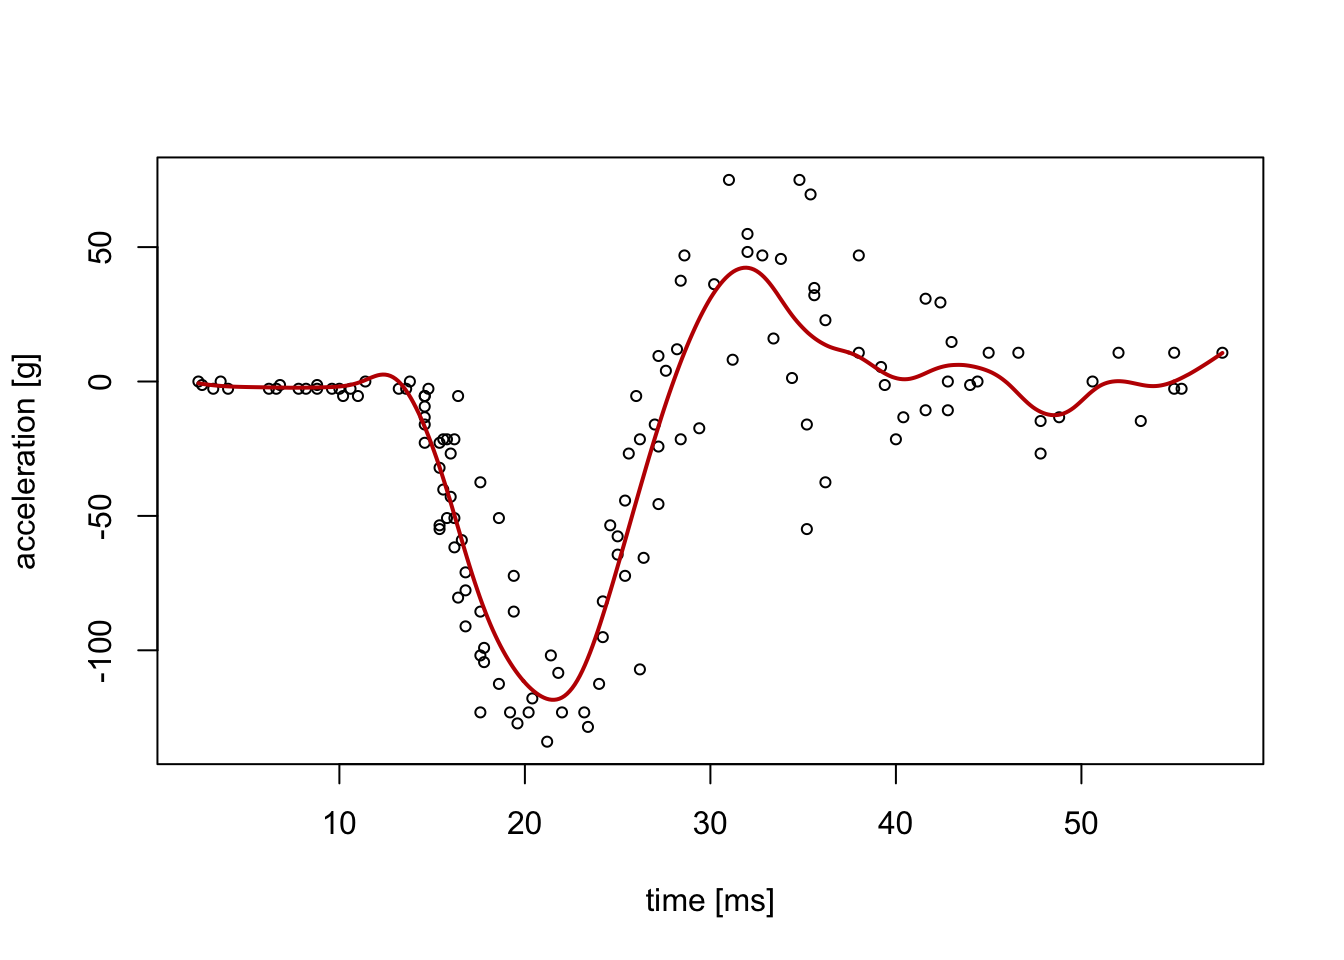
\includegraphics{MATH5714M_files/figure-latex/accel-1} 

}

\caption{An illustration of a dataset where a linear (straight line) model is not appropriate. The data represents a series of measurements of head acceleration in a simulated motorcycle accident, used to test crash helmets (the \texttt{mcycle} dataset from the \texttt{MASS} R package).}\label{fig:accel}
\end{figure}

\clearpage

\hypertarget{X01-KDE}{%
\section{Kernel Density Estimation}\label{X01-KDE}}

In this section we discuss the topic of ``Kernel Density Estimation''.
Here we suppose we are given data \(x_1,\ldots, x_n \in\mathbb{R}^d\) from an
unknown probability density, say \(f\). Our objective is to estimate
the density~\(f\). This section lays the foundations for many of the
following topics.

\hypertarget{histograms}{%
\subsection{Histograms}\label{histograms}}

\hypertarget{probability-densities}{%
\subsubsection{Probability Densities}\label{probability-densities}}

Before we consider how to estimate a density, let just remember what a
density is. A random variable \(X \in \mathbb{R}\) has \textbf{density} \(f\colon \mathbb{R}\to [0, \infty)\) if
\begin{equation*}
  P\bigl(X \in [a,b]\bigr)
  = \int_a^b f(x) \,dx
\end{equation*}
for all \(a, b\in\mathbb{R}\) with \(a < b\). Densities are sometimes also called
``probability densities'' or even ``probability density functions''.

A density \(f\) is large in regions where \(X\) is very likely to take
values, and small in regions where \(X\) is less likely to take values.
If \(f(x) = 0\) for all \(x\) in a region, that means that \(X\) never takes
values there. Graphically, the integral \(\int_a^b f(x) \,dx\) can be
interpreted as the area under the graph of~\(f\). This is illustrated
in figure~\ref{fig:density}.



\begin{figure}

{\centering 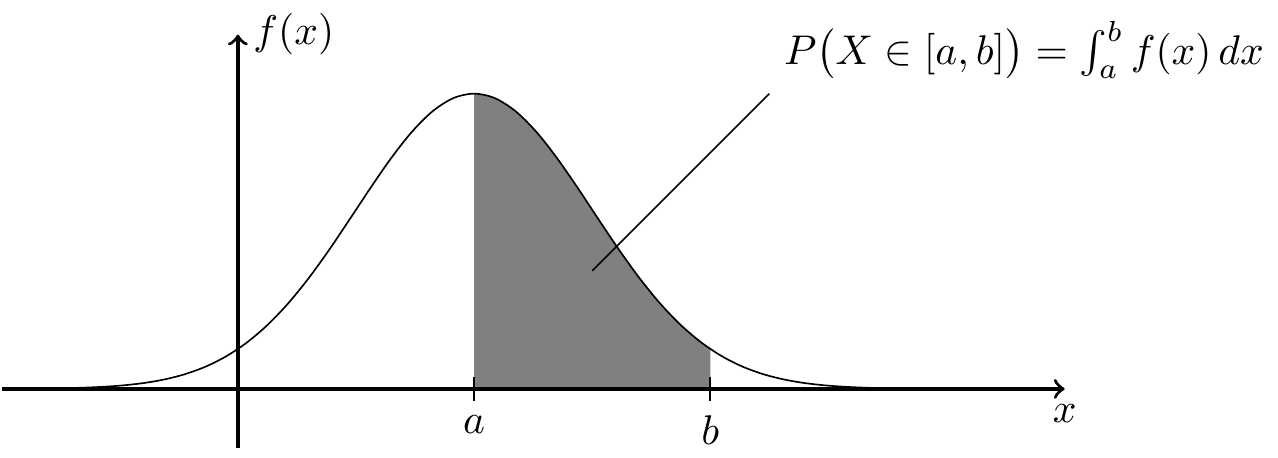
\includegraphics{MATH5714M_files/figure-latex/density-1} 

}

\caption{An illustration of how the area under the graph of a density can be interpreted as a probability.}\label{fig:density}
\end{figure}

A function \(f\) is the density of some random variable~\(X\),
if and only if \(f \geq 0\) and
\begin{equation*}
  \int_{-\infty}^\infty f(x) \,dx = 1.
\end{equation*}

\hypertarget{histograms-1}{%
\subsubsection{Histograms}\label{histograms-1}}

In the univariate case, \emph{i.e.}~for \(d = 1\), a commonly used technique
to approximate density of a sample is to plot a histogram. To
illustrate this, we use the \texttt{faithful} dataset built in R, which
contains waiting times between eruptions and the duration of the
eruption for the Old Faithful geyser in the Yellowstone National Park.
(You can type \texttt{help(faithful)} in R to learn more about this data
set.) Here we focus on the waiting times only. A simple histogram
for this dataset is shown in figure~\ref{fig:hist}.



\begin{Shaded}
\begin{Highlighting}[]
\NormalTok{x }\OtherTok{\textless{}{-}}\NormalTok{ faithful}\SpecialCharTok{$}\NormalTok{waiting}
\FunctionTok{hist}\NormalTok{(x, }\AttributeTok{probability =} \ConstantTok{TRUE}\NormalTok{,}
     \AttributeTok{main =} \ConstantTok{NULL}\NormalTok{, }\AttributeTok{xlab =} \StringTok{"time between eruptions [mins]"}\NormalTok{)}
\end{Highlighting}
\end{Shaded}

\begin{figure}
\centering
\includegraphics{MATH5714M_files/figure-latex/hist-1.pdf}
\caption{\label{fig:hist}This figure shows how a histogram can be used to approximate a probability density. From the plot one can see that the density of the waiting times distribution seems to be bi-modal with peaks around 53 and 80 minutes.}
\end{figure}

The histograms splits the range of the data into ``buckets'', and for
every bucket \([a, b]\) it shows a bar where the height is proportional
the number of samples in the bucket. I am ignoring the case that a
sample may fall exactly on the boundary between two buckets here; in
reality all but one buckets need to be half-open intervals, for
example \([40, 45]\), \((45, 50]\), \ldots, \((95, 100]\).

As we have seen, the area under the graph of the density \(f\) over the
interval \([a, b]\) corresponds to the probability~\(P\bigl(X \in [a,b]\bigr)\). For the histogram to approximate the density, we need
to scale the height \(h_{a,b}\) of the bucket \([a, b]\) so that the area
in the histogram is also close to this probability. Since we don't
know the probability \(P\bigl(X \in [a,b]\bigr)\) exactly, we have to
approximate it as
\begin{equation*}
  P\bigl(X \in [a,b]\bigr)
  \approx \frac{n_{a,b}}{n},
\end{equation*}
where \(n_{a,b}\) is the number of samples in the bucket \([a,b]\),
and \(n\) is the total number of samples. So we need
\begin{align*}
  (b-a) \cdot h_{a,b}
    &= \mbox{area of the histogram bar} \\
    &\approx \mbox{area of the density} \\
    &= P\bigl(X \in [a,b]\bigr) \\
    &\approx \frac{n_{a,b}}{n}.
\end{align*}
and thus we choose
\begin{equation*}
  h_{a,b}
  = \frac{1}{(b - a) n} n_{a,b}.
\end{equation*}
As expected, the height of the bar for the bucket \([a,b]\) is proportional
to the number \(n_{a,b}\) of samples in the bucket.

\hypertarget{choice-of-buckets}{%
\subsubsection{Choice of Buckets}\label{choice-of-buckets}}

Histograms are only meaningful if the buckets are chosen well. If
the buckets are too large, not much of the structure of \(f\) can be
resolved. If the buckets are too small, the estimate \(P\bigl(X \in [a,b]\bigr) \approx n_{a,b}/n\) will be poor and the histogram will
no longer resemble the shape of~\(f\). This



\begin{Shaded}
\begin{Highlighting}[]
\FunctionTok{set.seed}\NormalTok{(}\DecValTok{1}\NormalTok{)}
\NormalTok{x }\OtherTok{\textless{}{-}} \FunctionTok{rnorm}\NormalTok{(}\DecValTok{50}\NormalTok{)}
\FunctionTok{hist}\NormalTok{(x, }\AttributeTok{probability =} \ConstantTok{TRUE}\NormalTok{, }\AttributeTok{main =} \ConstantTok{NULL}\NormalTok{,}
     \AttributeTok{breaks =} \FunctionTok{seq}\NormalTok{(}\SpecialCharTok{{-}}\FloatTok{2.5}\NormalTok{, }\FloatTok{2.5}\NormalTok{, }\AttributeTok{length.out =} \DecValTok{500}\NormalTok{))}
\end{Highlighting}
\end{Shaded}

\begin{figure}
\centering
\includegraphics{MATH5714M_files/figure-latex/broken-hist-1.pdf}
\caption{\label{fig:broken-hist}This figure demonstrates the consequences of choosing a way too small bucket size.}
\end{figure}

Finally, even if reasonable bucket sizes are chosen, the result can
depend quite strongly on the exact locations of these buckets. To illustrate
this effect, we consider a
\href{https://teaching.seehuhn.de/data/buffalo/}{dataset about the annual amount of snow}
falling in Buffalo, New York for different years. Figures \ref{fig:buffalo1}
and~\ref{fig:buffalo2} show that same data in two different ways,
allowing to come to different conclusions about the distribution.



\begin{Shaded}
\begin{Highlighting}[]
\CommentTok{\# downloaded from https://teaching.seehuhn.de/data/buffalo/}
\NormalTok{x }\OtherTok{\textless{}{-}} \FunctionTok{read.csv}\NormalTok{(}\StringTok{"data/buffalo.csv"}\NormalTok{)}
\NormalTok{snowfall }\OtherTok{\textless{}{-}}\NormalTok{ x}\SpecialCharTok{$}\NormalTok{snowfall}
\FunctionTok{hist}\NormalTok{(snowfall, }\AttributeTok{probability =} \ConstantTok{TRUE}\NormalTok{,}
     \AttributeTok{breaks =} \FunctionTok{seq}\NormalTok{(}\FloatTok{24.30}\NormalTok{, }\FloatTok{208.22}\NormalTok{, }\AttributeTok{length.out =} \DecValTok{20}\NormalTok{),}
     \AttributeTok{main =} \ConstantTok{NULL}\NormalTok{, }\AttributeTok{xlab =} \StringTok{"snowfall [in]"}\NormalTok{)}
\end{Highlighting}
\end{Shaded}

\begin{figure}
\centering
\includegraphics{MATH5714M_files/figure-latex/buffalo1-1.pdf}
\caption{\label{fig:buffalo1}The annual amount of snowfall in Buffalo, New York, in inches. The histogram makes it plausible that there is one main peak in the distribution.}
\end{figure}



\begin{Shaded}
\begin{Highlighting}[]
\FunctionTok{hist}\NormalTok{(snowfall, }\AttributeTok{probability =} \ConstantTok{TRUE}\NormalTok{,}
     \AttributeTok{breaks =} \FunctionTok{seq}\NormalTok{(}\FloatTok{22.85}\NormalTok{, }\FloatTok{204.92}\NormalTok{, }\AttributeTok{length.out =} \DecValTok{20}\NormalTok{),}
     \AttributeTok{main =} \ConstantTok{NULL}\NormalTok{, }\AttributeTok{xlab =} \StringTok{"snowfall [in]"}\NormalTok{)}
\end{Highlighting}
\end{Shaded}

\begin{figure}
\centering
\includegraphics{MATH5714M_files/figure-latex/buffalo2-1.pdf}
\caption{\label{fig:buffalo2}Continued from \ref{fig:buffalo1}, this histogram shows the dataset in a way that three peaks are visible.}
\end{figure}

As a further illustration of the effect of bucket width, the code in
figure~\ref{fig:snow-hist-col} shows how histograms with different
bucket widths can be generated in~R. Here we simply specify numeric
values for the \texttt{break} argument to \texttt{hist()}, which R uses as the
\emph{approximate} number of buckets in the plot.



\begin{Shaded}
\begin{Highlighting}[]
\FunctionTok{par}\NormalTok{(}\AttributeTok{mfrow =} \FunctionTok{c}\NormalTok{(}\DecValTok{2}\NormalTok{,}\DecValTok{2}\NormalTok{))}

\ControlFlowTok{for}\NormalTok{ (breaks }\ControlFlowTok{in} \FunctionTok{c}\NormalTok{(}\DecValTok{80}\NormalTok{, }\DecValTok{40}\NormalTok{, }\DecValTok{20}\NormalTok{, }\DecValTok{10}\NormalTok{)) \{}
  \FunctionTok{hist}\NormalTok{(snowfall,}
       \AttributeTok{prob =} \ConstantTok{TRUE}\NormalTok{,}
       \AttributeTok{breaks =}\NormalTok{ breaks,}
       \AttributeTok{xlim =} \FunctionTok{c}\NormalTok{(}\DecValTok{25}\NormalTok{,}\DecValTok{200}\NormalTok{),}
       \AttributeTok{ylim =} \FunctionTok{c}\NormalTok{(}\DecValTok{0}\NormalTok{, }\FloatTok{0.03}\NormalTok{),}
       \AttributeTok{xlab =} \FunctionTok{paste}\NormalTok{(}\StringTok{"breaks ="}\NormalTok{, breaks),}
       \AttributeTok{main =} \ConstantTok{NULL}\NormalTok{)}
\NormalTok{\}}
\end{Highlighting}
\end{Shaded}

\begin{figure}
\centering
\includegraphics{MATH5714M_files/figure-latex/snow-hist-col-1.pdf}
\caption{\label{fig:snow-hist-col}This figure illustrates how the bucket size in a histogram can be controlled in R.}
\end{figure}

\hypertarget{kernel-density-estimation}{%
\subsection{Kernel Density Estimation}\label{kernel-density-estimation}}

Kernel density estimation allows to estimate the density \(f\) for given
data while avoiding some of the disadvantages of histograms.
Again, we suppose that we are given data \(x_1, \ldots, x_n \in \mathbb{R}\)
and that we want to estimate the density \(f\).

\hypertarget{motivation}{%
\subsubsection{Motivation}\label{motivation}}

Similar to the argument in the previous subsection, for \(x\) in a ``small''
interval \([a,b]\) we can estimate \(f(x)\) as
\begin{equation*}
  f(x)
  \approx \frac{1}{b-a} \int_a^b f(y) \,dy
  = \frac{1}{b-a} P\bigl( X\in [a,b] \bigr)
  \approx \frac{1}{b-a} \frac{n_{a,b}}{n},
\end{equation*}
where \(n_{a,b}\) denotes the number of samples in the interval \([a, b]\).
This equation contains two approximation. The first one,
\(f(x) \approx 1/(ba) \int_a^b f(y) \,dy\), is more accurate if the
interval is small, because then \(f\) will be nearly constant over the
interval. The second approximation will be more accurate if the
interval is large, because then the interval \([a,b]\) covers more samples
and the estimate of the probability is based on more data. We will later
discuss in detail how these two concerns can be optimally balanced.

A mathematical ``trick'' to write more clearly how \(n_{a,b}\) depends on the
data is to write the value as
\begin{equation*}
  n_{a,b}
  = \sum_{i=1}^n I_{[a,b]}(x_i),
\end{equation*}
where
\begin{equation*}
  I_{[a,b]}(x)
  = \begin{cases}
    1 & \mbox{if $x \in [a,b]$, and} \\
    0 & \mbox{otherwise.}
  \end{cases}
\end{equation*}
The function \(I_{[a,b]}\) is called the \textbf{indicator function} of the
set~\([a, b]\).

Using the indicator function notation, the estimate for \(f(x)\)
can be written as
\begin{align*}
  f(x)
  \approx \frac{1}{n(b-a)} n_{a,b}
  = \frac{1}{n} \sum_{i=1}^n \frac{1}{b-a} I_{[a,b]}(x_i)
\end{align*}
whenever \(x \in [a,b]\) and when \(b-a\) is ``not too large and not too small''.
For symmetry we choose the interval \([a, b]\) centred around \(x\),
say \([a, b] = [x - h, x + h]\) where \(h\) can be chosen to control the
width of the interval. In this case we have \(b - a = x + h - x + h = 2h\) and thus
\begin{align*}
  f(x)
  &\approx \frac{1}{n} \sum_{i=1}^n \frac{1}{2h} I_{[x-h,x+h]}(x_i) \\
  &= \frac{1}{n} \sum_{i=1}^n \frac{1}{2h} I_{[-h,+h]}(x_i-x) \\
  &= \frac{1}{n} \sum_{i=1}^n \frac{1}{2h} I_{[-1,+1]}\Bigl(\frac{x_i-x}{h}\Bigr)
\end{align*}
for all \(x \in \mathbb{R}\). This is an example of a kernel density estimate.
The function \(K(x) = 1/2 \, I_{[-1,+1]}(x)\) on the right-hand side is
called the kernel of the estimate, and the parameter \(h\) is called the
\textbf{bandwidth} or the smoothing parameter.

\hypertarget{definition-of-a-kernel-density-estimator}{%
\subsubsection{Definition of a Kernel Density Estimator}\label{definition-of-a-kernel-density-estimator}}

The general kernel density estimate is a generalisation of the idea
from the previous subsection. We first define the class of functions
which we use to replace the function \(1/2 \, I_{[-1,+1]}\).

\begin{definition}
\protect\hypertarget{def:kernel}{}\label{def:kernel}

A \textbf{kernel} is a function \(K\colon \mathbb{R}\to \mathbb{R}\) such that

\begin{itemize}
\tightlist
\item
  \(\int_{-\infty}^\infty K(x) \,dx = 1\),
\item
  \(K(x) = K(-x)\) (i.e.~\(K\) is \emph{symmetric}) and
\item
  \(K(x) \geq 0\) (i.e.~\(K\) is \emph{positive}) for all \(x\in \mathbb{R}\).
\end{itemize}

\end{definition}

Of these three properties, the first one is the most important one.
The second condition, symmetry, ensures that \(K\) is centred around \(0\)
and the third definition, positivity, makes \(K\) a probability density.
(While most authors list all three properties shown above, sometimes
the third condition is omitted.)

It is easy to check that \(K(x) = 1/2 \, I_{[-1,+1]}(x)\) satisfies all
three conditions of definition~\ref{def:kernel}. This function \(K\)
is sometimes called the ``uniform kernel'', because it is the density
of the uniform distribution~\(\mathcal{U}[-1,+1]\).

Based on the concept of a kernel, we now can define
what a Kernel Density Estimate is.

\begin{definition}
\protect\hypertarget{def:KDE}{}\label{def:KDE}For a kernel~\(K\), bandwidth~\(h > 0\) and \(x \in \mathbb{R}\), the
\textbf{kernel density estimate} for \(f(x)\) is given by
\begin{equation*}
  \hat f_h(x)
  = \frac{1}{n} \sum_{i=1}^n K_h(x - x_i),
\end{equation*}
where \(K_h\) is given by
\begin{equation*}
  K_h(y)
  = \frac{1}{h} K(y/h)
\end{equation*}
for all \(y\in \mathbb{R}\).
\end{definition}

For \(K(x) = 1/2 \, I_{[-1,+1]}(x)\) this definition recovers the
approximation we discussed in the previous section. In later sections
we will see how the kernel \(K\) can be chosen for the estimator \(\hat f\) to have ``good'' properties. As a simple example we note that if \(K\)
is continuous, then the rescaled kernel \(K_h\) and thus also the
estimate \(f_h\) are continuous functions.

Similar to the bucket width in histograms, the bandwidth parameter~\(h\)
controls how smooth the density estimate~\(\hat f_h\) is, as a function
of~\(x\).

\hypertarget{kernels}{%
\subsubsection{Kernels}\label{kernels}}

There are many different kernels in use. Some examples are listed
below. A more exhautive list can, for example, be found
\href{https://en.wikipedia.org/wiki/Kernel_(statistics)\#Kernel_functions_in_common_use}{on Wikipedia}.

\hypertarget{uniform-kernel}{%
\paragraph{Uniform Kernel}\label{uniform-kernel}}

\begin{equation*}
  K(x)
  = \begin{cases}
      1/2 & \mbox{if $-1 \leq x \leq 1$} \\
      0 & \mbox{otherwise}
    \end{cases}
\end{equation*}

\includegraphics{MATH5714M_files/figure-latex/kUniform-1.pdf}

\hypertarget{triangular-kernel}{%
\paragraph{Triangular Kernel}\label{triangular-kernel}}

\begin{equation*}
  K(x)
  = \begin{cases}
      1-|x| & \mbox{if $-1 \leq x \leq 1$} \\
      0 & \mbox{otherwise}
    \end{cases}
\end{equation*}

\includegraphics{MATH5714M_files/figure-latex/kTriangular-1.pdf}

\hypertarget{epanechnikov-kernel}{%
\paragraph{Epanechnikov Kernel}\label{epanechnikov-kernel}}

\begin{equation*}
  K(x)
  = \begin{cases}
      \frac34 (1-x^2) & \mbox{if $-1 \leq x \leq 1$} \\
      0 & \mbox{otherwise}
    \end{cases}
\end{equation*}

\includegraphics{MATH5714M_files/figure-latex/kEpanechnikov-1.pdf}

\hypertarget{gaussian-kernel}{%
\paragraph{Gaussian Kernel}\label{gaussian-kernel}}

\begin{equation*}
  K(x)
  = \frac{1}{\sqrt{2\pi}} \exp\bigl(-x^2/2\bigr)
\end{equation*}

\includegraphics{MATH5714M_files/figure-latex/kGaussian-1.pdf}

\hypertarget{kernel-density-estimation-in-r}{%
\subsection{Kernel Density Estimation in R}\label{kernel-density-estimation-in-r}}

Kernel density estimates can be computed in R using the built-in
\texttt{density()} function. If \texttt{x} is a vector containing the data, then
\texttt{density(x)} computes a basic kernel density estimate, using the
Gaussian kernel. The function has a number of optional arguments,
which can be used to control details of the estimate:

\begin{itemize}
\item
  \texttt{bw\ =\ ...} can be used to control the bandwidth~\(h\).
  If no numeric value is given, a heuristic is used.
  Note that for some kernels, \texttt{bw} differs from our \(h\)
  by a constant factor. The value \texttt{bw=1} always corresponds
  to the case where the probability distribution with density
  \(K_h\) has variance~1.
\item
  \texttt{kernel\ =\ ...} can be used to choose the kernel.
  Choices incluse \texttt{"rectangular"} (the uniform kernel), \texttt{"triangular"},
  \texttt{"epanechnikov"} and \texttt{"gaussian"}.
\end{itemize}

Details about how to call \texttt{density()} can be found by using the
\href{https://rdrr.io/r/stats/density.html}{command \texttt{help(density)}} in R.

The return value of \texttt{density} is an R object which contains information
about the kernel density estimate.

\begin{Shaded}
\begin{Highlighting}[]
\NormalTok{m }\OtherTok{\textless{}{-}} \FunctionTok{density}\NormalTok{(snowfall)}
\FunctionTok{str}\NormalTok{(m)}
\end{Highlighting}
\end{Shaded}

\begin{verbatim}
## List of 7
##  $ x        : num [1:512] -4.17 -3.72 -3.26 -2.81 -2.35 ...
##  $ y        : num [1:512] 4.32e-06 4.98e-06 5.73e-06 6.56e-06 7.48e-06 ...
##  $ bw       : num 9.72
##  $ n        : int 109
##  $ call     : language density.default(x = snowfall)
##  $ data.name: chr "snowfall"
##  $ has.na   : logi FALSE
##  - attr(*, "class")= chr "density"
\end{verbatim}

The field \texttt{\$x} and \texttt{\$y} contain the \(x\) and~\(y\) coordinates, respectively,
of points on the \(x \mapsto \hat f_h(x)\) curve, which approximates~\(f\).
The field \texttt{\$bw} shows the numeric value for the bandwidth chosen by
the heuristic. The returned object can also directly be used
as an argument to \texttt{plot()} and \texttt{lines()}, to add the graph of \(\hat f_h\)
to a plot. The commands in figure~\ref{fig:snow-dens-col} show how the
command \texttt{density()} can be used and illustrate the effect of the
bandwidth parameter.



\begin{Shaded}
\begin{Highlighting}[]
\FunctionTok{par}\NormalTok{(}\AttributeTok{mfrow =} \FunctionTok{c}\NormalTok{(}\DecValTok{2}\NormalTok{,}\DecValTok{2}\NormalTok{))}

\ControlFlowTok{for}\NormalTok{ (bw }\ControlFlowTok{in} \FunctionTok{c}\NormalTok{(}\DecValTok{1}\NormalTok{, }\DecValTok{2}\NormalTok{, }\DecValTok{4}\NormalTok{, }\DecValTok{8}\NormalTok{)) \{}
  \FunctionTok{plot}\NormalTok{(}\FunctionTok{density}\NormalTok{(snowfall, }\AttributeTok{bw =}\NormalTok{ bw, }\AttributeTok{kernel =} \StringTok{"triangular"}\NormalTok{, }\AttributeTok{n =} \DecValTok{1000}\NormalTok{),}
    \AttributeTok{xlim =} \FunctionTok{c}\NormalTok{(}\DecValTok{25}\NormalTok{,}\DecValTok{200}\NormalTok{),}
    \AttributeTok{ylim =} \FunctionTok{c}\NormalTok{(}\DecValTok{0}\NormalTok{, }\FloatTok{0.03}\NormalTok{),}
    \AttributeTok{xlab =} \FunctionTok{paste}\NormalTok{(}\StringTok{"bandwidth ="}\NormalTok{, bw),}
    \AttributeTok{main =} \ConstantTok{NA}\NormalTok{)}
\NormalTok{\}}
\end{Highlighting}
\end{Shaded}

\begin{figure}
\centering
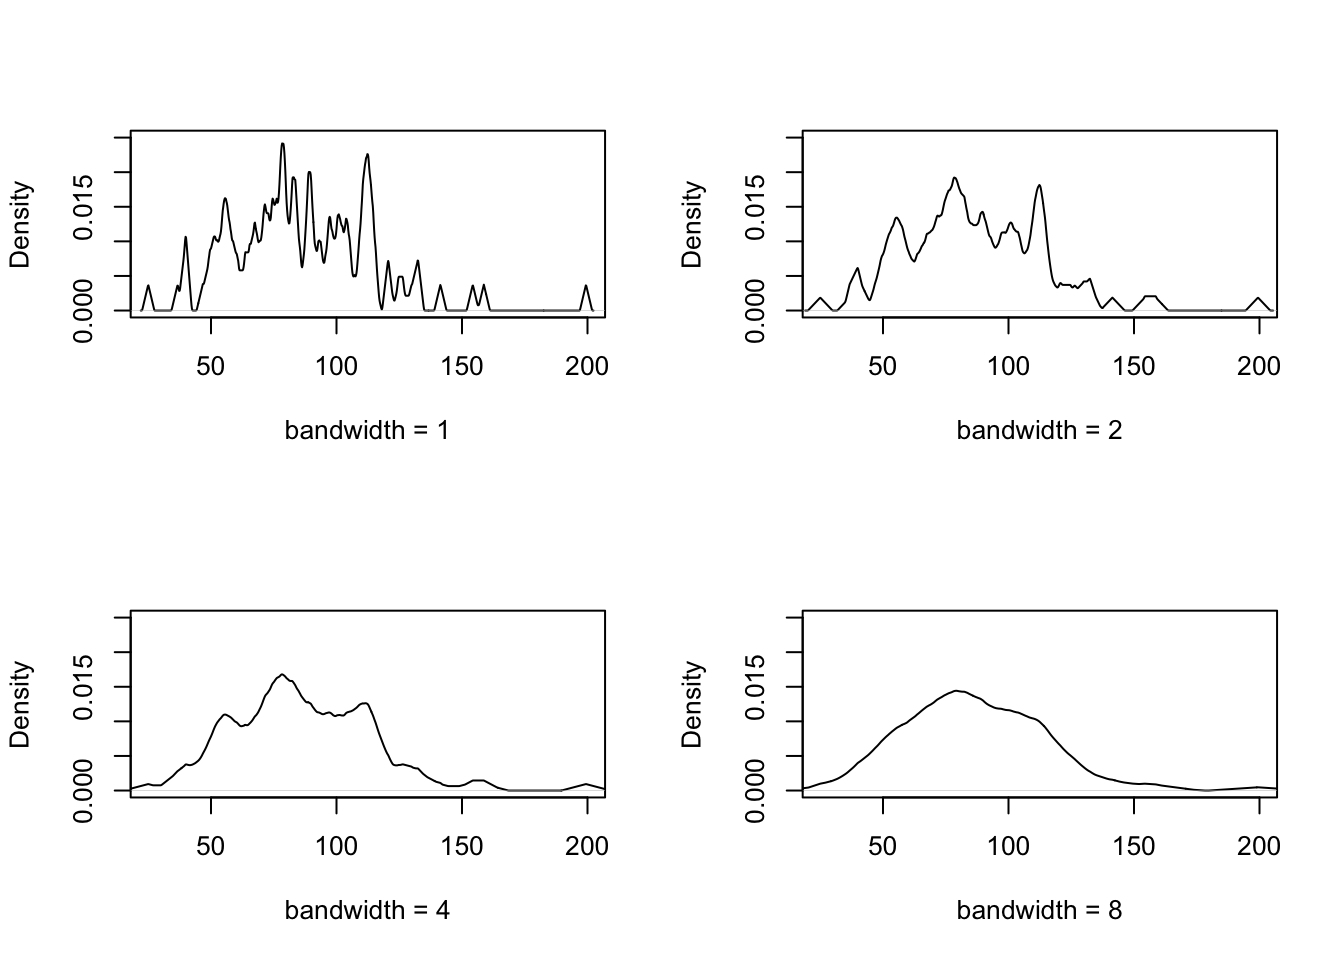
\includegraphics{MATH5714M_files/figure-latex/snow-dens-col-1.pdf}
\caption{\label{fig:snow-dens-col}This figure illustrates how the bandwidth of a kernel density estimate can be controlled in R.}
\end{figure}

\textbf{Summary}

\begin{itemize}
\tightlist
\item
  Histograms can be scaled so that they approximate densities.
\item
  Some care is needed when choosing buckets for a histogram.
\item
  Kernel density estimates can be used to estimate densities from data.
\item
  A variety of different kernel functions are commonly used.
\end{itemize}

\clearpage

\hypertarget{X02-Bias}{%
\section{The Bias of Kernel Density Estimates}\label{X02-Bias}}

In the previous section we introduced the kernel density estimate
\begin{equation}
  \hat f_h(x)
  = \frac{1}{n} \sum_{i=1}^n K_h(x - x_i)  \label{eq:KDE-est}
\end{equation}
for estimating the density \(f\), and we argued that \(\hat f_h(x) \approx f(x)\).
The aim of the current section is to quantify the error of this approximation
and to understand how this error depends on the true density~\(f\)
and on the bandwidth~\(h > 0\).

\hypertarget{a-statistical-model}{%
\subsection{A Statistical Model}\label{a-statistical-model}}

As usual, we will make a statistical model for the data \(x_1, \ldots, x_n\),
and then use this model to analyse how well the estimator performs.
The statistical model we will consider here is extremely simple: we
model the \(x_i\) using random variables
\begin{equation}
  X_1, \ldots, X_n \sim f,  \label{eq:KDE-model}
\end{equation}
which we assume to be independent and identically distributed (i.i.d.).
Here, the notation \(X \sim f\), where \(f\) is a probability density, simply
denotes that the random variable \(X\) has density~\(f\).

It is important to not confuse \(x\) (the point where we are evaluating
the densities during our analysis) with the data \(x_i\). A statistical
model describes the data, so here we get random variables \(X_1, \ldots, x_n\)
to describe the behaviour of \(x_1, \ldots, x_n\), but it does not descibe \(x\).
The number \(x\) is not part of the data, so will never be modelled by a
random variable.

While the model is very simple, for example it is much simpler than the
model we use in the level 3 part of the module for linear regression,
the associated parameter estimation problem is more challenging.
The only ``parameter'' in this model is the function \(f \colon\mathbb{R}\to \mathbb{R}\)
instead of just a vector of numbers. The space of all possible density
functions \(f\) is infinite dimensional, so this is a more challenging
estimation problem then the one we consider, for example, for linear
regression. Since \(f\) is not a ``parameter'' in the usual sense, sometimes
this problem is called a ``non-parametric'' estimation problem.

Our estimate for the density \(f\) is the function \(\hat f_h\colon \mathbb{R}\to \mathbb{R}\),
where \(\hat f_h(x)\) is given by~\eqref{eq:KDE-est} for every \(x \in\mathbb{R}\).

\hypertarget{the-bias-of-the-estimate}{%
\subsection{The Bias of the Estimate}\label{the-bias-of-the-estimate}}

As ususal, the \textbf{bias} of our estimate is the difference between
what the estimator gives on average and the truth. For our estimation
problem we get
\begin{equation*}
    \mathop{\mathrm{bias}}\bigl(\hat f_h(x)\bigr)
    = \mathbb{E}\bigl(\hat f_h(x)\bigr) - f(x).
\end{equation*}
The expectation on the right-hand side averages over the randomness
in the data, by using \(X_1, \ldots, X_n\) from the model in place of
the data.

Substituting in the definition of \(\hat f_h(x)\) from equation~\eqref{eq:KDE-est}
we find
\begin{align*}
    \mathbb{E}\bigl(\hat f_h(x)\bigr)
    &= \mathbb{E}\Bigl( \frac{1}{n} \sum_{i=1}^n K_h(x - X_i) \Bigr) \\
    &= \frac{1}{n} \sum_{i=1}^n \mathbb{E}\bigl( K_h(x - X_i) \bigr)
\end{align*}
and since the \(X_i\) are identically distributed, we can replace
all \(X_i\) with \(X_1\) (or any other of them) to get
\begin{align*}
    \mathbb{E}\bigl(\hat f_h(x)\bigr)
    &= \frac{1}{n} \sum_{i=1}^n \mathbb{E}\bigl( K_h(x - X_1) \bigr) \\
    &= \frac{1}{n} n \, \mathbb{E}\bigl( K_h(x - X_1) \bigr) \\
    &= \mathbb{E}\bigl( K_h(x - X_1) \bigr).
\end{align*}
Since the model assumes \(X_1\) (and all the other \(X_i\)) to have density~\(f\),
we can write this expectation as an integral to get
\begin{align*}
    \mathbb{E}\bigl(\hat f_h(x)\bigr)
    &= \int_{-\infty}^\infty K_h(x - y) \, f(y) \, dy \\
    &= \int_{-\infty}^\infty f(y) \, K_h(y - x) \, dy \\
    &= \int_{-\infty}^\infty f(z+x) \, K_h(z) \, dz
\end{align*}
where we used the symmetry of \(K_h\) and the substitution \(z = y - x\).

\hypertarget{moments-of-kernels}{%
\subsection{Moments of Kernels}\label{moments-of-kernels}}

To understand how the bias changes as \(h\) varies, we will need to
consider properties of \(K\) and \(K_h\) in more detail.

\begin{definition}
The \(k\)th \textbf{moment} of a kernel~\(K\),
for \(k \in \mathbb{N}_0 = \{0, 1, 2, \ldots\}\), is given by
\begin{equation*}
  \mu_k(K)
  = \int_{-\infty}^\infty x^k K(x) \,dx.
\end{equation*}
\end{definition}

The second moment \(\mu_2\) is sometimes also called the \emph{variance}
of the kernel~\(K\).

Using the properties of \(K\), we find the following results:

\begin{itemize}
\item
  Since \(x^0 = 1\) for all \(x\in\mathbb{R}\),
  the \(0\)th moment is \(\mu_0(K) = \int_{-\infty}^\infty K(x) \,dx = 1\)
  for every kernel~\(K\).
\item
  Since \(K\) is symmetric, the function \(x \mapsto x K(x)\) is
  antisymmetric and we have
  \begin{equation*}
    \mu_1(K)
    = \int_{-\infty}^\infty x K(x) \,dx
    = 0
  \end{equation*}
  for every kernel~\(K\).
\end{itemize}

The moments of the rescaled kernel \(K_h\), given by
\begin{equation*}
    K_h(x - y)
    = \frac{1}{h} K\Bigl( \frac{x-y}{h} \Bigr),
\end{equation*}
can be computed from the moments of \(K\).

\begin{lemma}
\protect\hypertarget{lem:Kh-scal}{}\label{lem:Kh-scal}Let \(K\) be a kernel, \(k \in \mathbb{N}_0\) and \(h > 0\). Then
\begin{equation*}
  \mu_k(K_h)
  = h^k \mu_k(K).
\end{equation*}
\end{lemma}

\begin{proof}
We have
\begin{align*}
  \mu_k(K_h)
  &= \int_{-\infty}^\infty x^k K_h(x) \,dx \\
  &= \int_{-\infty}^\infty x^k \frac1h K\Bigl(\frac{x}{h}\Bigr) \,dx.
\end{align*}
Using the substitution \(y = x/h\) we find
\begin{align*}
  \mu_k(K_h)
  &= \int_{-\infty}^\infty (hy)^k \frac1h K(y) \, h \,dy \\
  &= h^k \int_{-\infty}^\infty y^k K(y) \,dy \\
  &= h^k \mu_k(K).
\end{align*}
This completes the proof.
\end{proof}

It is easy to check that if \(K\) is a kernel, then \(K_h\) is also a kernel which
implies that \(K_h\) is a probability density. If \(Y\) is a random variable with
density \(K_h\), written as \(Y \sim K_h\) in short, then we find
\begin{equation*}
  \mathbb{E}(Y)
  = \int y K_h(y) \,dy
  = \mu_1(K_h)
  = 0
\end{equation*}
and
\begin{equation}
  \mathop{\mathrm{Var}}(Y)
  = \mathbb{E}(Y^2)
  = \int y^2 K_h(y) \,dy
  = \mu_2(K_h)
  = h^2 \, \mu_2(K).  \label{eq:Kh-var-Y}
\end{equation}
Thus, \(Y\) is centred and the variance of \(Y\) is proportional to~\(h^2\).

\hypertarget{the-bias-for-small-bandwidth}{%
\subsection{The Bias for Small Bandwidth}\label{the-bias-for-small-bandwidth}}

Considering again the formula
\begin{equation*}
    \mathbb{E}\bigl(\hat f_h(x)\bigr)
    = \int_{-\infty}^\infty f(x+y) \, K_h(y) \, dy,
\end{equation*}
we see that we can interpret this integral as an expectation
with respect to a random variable \(Y \sim K_h\):
\begin{equation}
    \mathbb{E}\bigl(\hat f_h(x)\bigr)
    = \mathbb{E}\bigl( f(x+Y) \bigr).  \label{eq:hf2}
\end{equation}
Equation~\eqref{eq:Kh-var-Y} shows that for \(h \downarrow 0\) the random
variable concentrates more and more around \(0\) and thus \(x+Y\) concentrates
more and more around~\(x\). For this reason we
expect~\(\mathbb{E}\bigl(\hat f_h(x)\bigr) \approx f(x)\) for small~\(h\).

To get a more qualitative version of this argument, we consider the
\href{https://en.wikipedia.org/wiki/Taylor\%27s_theorem}{Taylor approximation}
of \(f\) around the point~\(x\):
\begin{equation*}
  f(x + y)
  \approx f(x) + y f'(x) + \frac{y^2}{2} f''(x).
\end{equation*}
Substituting this into equation~\eqref{eq:hf2} we find
\begin{align*}
    \mathbb{E}\bigl(\hat f_h(x)\bigr)
    &\approx \mathbb{E}\Bigl( f(x) + Y f'(x) + \frac{Y^2}{2} f''(x) \Bigr) \\
    &= f(x) + \mathbb{E}(Y) f'(x) + \frac12 \mathbb{E}(Y^2) f''(x) \\
    &= f(x) + \frac12 h^2 \mu_2(K) f''(x)
\end{align*}
for small \(h\). Considering the bias again, this gives
\begin{equation}
  \mathop{\mathrm{bias}}\bigl( \hat f_h(x) \bigr)
  = \mathbb{E}\bigl( \hat f_h(x) \bigr) - f(x)
  \approx \frac{\mu_2(K) f''(x)}{2} h^2  \label{eq:fhatbias}
\end{equation}
which shows that the bias of the estimator descreases quadratically
as \(h\) gets smaller.

In contrast, we will see in the next section that the variance of the
estimator \emph{increases} as \(h \downarrow 0\). We will need to balance these
two effects to find the optimal value of~\(h\).

\textbf{Summary}

\begin{itemize}
\tightlist
\item
  We have introduced a statistical model for density estimation.
\item
  The bias for kernel density estimation can be written as an integral.
\item
  We learned how the moments of a kernel are defined.
\item
  The bias for small bandwidth depends on the second moment of the
  kernel and the second derivative of the density.
\end{itemize}

\clearpage

\hypertarget{X03-Var}{%
\section{The Variance of Kernel Density Estimates}\label{X03-Var}}

In the previous section we considered the bias of the estimator
\begin{equation*}
  \hat f_h(x)
  = \frac{1}{n} \sum_{i=1}^n K_h(x - x_i).
\end{equation*}
We found
\begin{equation}
  \mathbb{E}\bigl( \hat f_h(x) \bigr)
  = \mathbb{E}\bigl( K_h(x - X_i) \bigr)  \label{eq:E-hat-f-K-h}
\end{equation}
for all \(i \in \{1, \ldots, n\}\) (we used \(i=1\)), and we used this relation
to compute the bias. In this section, we will use similar arguments to compute
the variance and the mean squared error of the estimator.

\hypertarget{variance}{%
\subsection{Variance}\label{variance}}

We use the formula
\begin{equation*}
  \mathop{\mathrm{Var}}\bigl( \hat f_h(x) \bigr)
  = \mathbb{E}\bigl( \hat f_h(x)^2 \bigr) - \mathbb{E}\bigl( \hat f_h(x) \bigr)^2
\end{equation*}
and consider the two terms separately.

\hypertarget{second-moment}{%
\subsubsection{Second Moment}\label{second-moment}}

For the second moment term in the definition of the variance we get
\begin{align*}
  \mathbb{E}\bigl( \hat f_h(x)^2 \bigr)
  &= \mathbb{E}\Bigl( \frac{1}{n} \sum_{i=1}^n K_h(x - X_i) \frac{1}{n} \sum_{j=1}^n K_h(x - X_j) \Bigr) \\
  &= \frac{1}{n^2} \mathbb{E}\Bigl( \sum_{i,j=1}^n K_h(x - X_i) K_h(x - X_j) \Bigr) \\
  &= \frac{1}{n^2} \sum_{i,j=1}^n \mathbb{E}\Bigl( K_h(x - X_i) K_h(x - X_j) \Bigr)
\end{align*}
Since the \(X_i\) are independent, the values of \(i\) and \(j\) in this sum do not
matter. For the \(n\) terms where \(i=j\) we can assume that both indices equal
1, and for the \(n(n-1)\) terms where \(i\neq j\) we can assume \(i=1\) and \(j=2\),
without changing the value of the expectation. So we get
\begin{align*}
  \mathbb{E}\bigl( \hat f_h(x)^2 \bigr)
  &= \frac{1}{n^2} \Bigl( n \mathbb{E}\bigl( K_h(x - X_1)^2 ) + n(n-1) \mathbb{E}\bigl( K_h(x - X_1) K_h(x - X_2) \bigr) \Bigr) \\
  &= \frac{1}{n^2} \Bigl( n \mathbb{E}\bigl( K_h(x - X_1)^2 ) + n(n-1) \mathbb{E}\bigl( K_h(x - X_1) \bigr) \mathbb{E}\bigl( K_h(x - X_2) \bigr) \Bigr) \\
  &= \frac{1}{n^2} \Bigl( n \mathbb{E}\bigl( K_h(x - X_1)^2 ) + n(n-1) \mathbb{E}\bigl( K_h(x - X_1) \bigr)^2 \Bigr) \\
  &= \frac{1}{n} \mathbb{E}\Bigl( K_h(x - X_1)^2 \Bigr) + \frac{n-1}{n} \mathbb{E}\bigl( \hat f_h(x) \bigr)^2,
\end{align*}
where we used equation~\eqref{eq:E-hat-f-K-h} for the last term.
Using this equation, we can write the expectation as
\begin{align*}
  \mathop{\mathrm{Var}}\bigl( \hat f_h(x) \bigr)
  &= \mathbb{E}\bigl( \hat f_h(x)^2 \bigr) - \mathbb{E}\bigl( \hat f_h(x) \bigr)^2 \\
  &= \frac{1}{n} \mathbb{E}\bigl( K_h(x - X_1)^2 ) + \Bigl(\frac{n-1}{n} - 1\Bigr) \mathbb{E}\bigl( \hat f_h(x) \bigr)^2.
\end{align*}
Since \((n-1)/n - 1 = -1/n\) we get
\begin{equation}
  \mathop{\mathrm{Var}}\bigl( \hat f_h(x) \bigr)
  = \frac{1}{n} \Bigl( \mathbb{E}\bigl( K_h(x - X_1)^2 ) - \mathbb{E}\bigl( \hat f_h(x) \bigr)^2 \Bigr).
                                                          \label{eq:Var-hat-f-2}
\end{equation}

\hypertarget{the-roughness-of-a-kernel}{%
\subsubsection{The Roughness of a Kernel}\label{the-roughness-of-a-kernel}}

Similar to what we did in the last section, we will use Taylor expansion
of \(f\) around the point \(x\) to understand the behaviour of the variance
for small~\(h\). Some more care is needed here, because this time the
result also depends on the sample size~\(n\) and we will consider the joint
limit of \(n \to \infty\) and \(h\to 0\). For the first term in
equation~\eqref{eq:Var-hat-f-2} we find
\begin{align*}
  \mathbb{E}\bigl( K_h(x - X_1)^2 )
  &= \int K_h(x - y)^2 f(y) \,dy \\
  &= \int K_h(y - x)^2 f(y) \,dy \\
  &= \int \frac{1}{h^2} K\Bigl( \frac{y - x}{h} \Bigr)^2 f(y) \,dy.
\end{align*}
Now we use the substitution \(z = (y - x) / h\). This gives
\begin{align*}
  \mathbb{E}\bigl( K_h(x - X_1)^2 )
  &= \int \frac{1}{h^2} K(z)^2 f(x + hz) \,h \,dz
\end{align*}
Finally, we use Taylor approximation to get
\begin{align*}
  \mathbb{E}\bigl( K_h(x - X_1)^2 )
  &\approx \int \frac{1}{h} K(z)^2 \Bigl( f(x) + hz\,f'(x) + \frac12 h^2 z^2 \,f''(x) \Bigr) \,dz \\
  &= \frac{1}{h} f(x) \int K(z)^2 \,dz
      + f'(x) \int z K(z)^2 \,dz
      + \frac12 h f''(x) \int z^2 K(z)^2 \,dz \\
  &= \frac{1}{h} f(x) \int K(z)^2 \,dz
      + \frac12 h f''(x) \int z^2 K(z)^2 \,dz
\end{align*}
where the first-order term disappears since \(z \mapsto z K(z)^2\) is an
asymmetric function. As a shorthand we use the following definition.

\begin{definition}
The \textbf{roughness} of a kernel \(K\) is given by
\begin{equation*}
  R(K)
  := \int_{-\infty}^\infty K(x)^2 \,dx.
\end{equation*}
\end{definition}

This gives the result
\begin{equation}
  \mathbb{E}\bigl( K_h(x - X_1)^2 \bigr)
  \approx \frac{1}{h} f(x) R(K) + \frac12 h f''(x) \int z^2 K(z)^2 \,dz
                             \label{eq:Var-frag1}
\end{equation}
for small \(h\).

\hypertarget{the-variance-for-small-bandwidth}{%
\subsubsection{The Variance for Small Bandwidth}\label{the-variance-for-small-bandwidth}}

Here we consider the term \(\mathbb{E}\bigl( \hat f_h(x) \bigr)^2\) in the formula
for the variance. From the previous section we know
\begin{equation*}
    \mathbb{E}\bigl( \hat f_h(x) \bigr)
    \approx f(x) + \frac12 h^2 \mu_2(K) f''(x)
\end{equation*}
and thus we get
\begin{equation}
    \mathbb{E}\bigl( \hat f_h(x) \bigr)^2
    \approx f(x)^2 + h^2 \mu_2(K) f(x) f''(x) + \frac14 h^4 \mu_2(K)^2 f''(x)^2
                             \label{eq:Var-frag2}
\end{equation}
for small \(h\).

Substituting \eqref{eq:Var-frag1} and~\eqref{eq:Var-frag2} into
equation~\eqref{eq:Var-hat-f-2} we finally find
\begin{equation*}
  \mathop{\mathrm{Var}}\bigl( \hat f_h(x) \bigr)
  = \frac{1}{n} \Bigl(
    \frac{1}{h} f(x) R(K)
    - f(x)^2
    + \cdots
   \Bigr),
\end{equation*}
where all the omitted terms go to zero as \(h \downarrow 0\).
Omitting one more term and keeping only the leading term
we find
\begin{equation}
  \mathop{\mathrm{Var}}\bigl( \hat f_h(x) \bigr)
  \approx \frac{1}{nh} f(x) R(K)     \label{eq:fhatvar}
\end{equation}
as~\(h\downarrow 0\).

\hypertarget{mean-squared-error}{%
\subsection{Mean Squared Error}\label{mean-squared-error}}

The Mean Squared Error of the estimator \(\hat f_h(x)\) for \(f(x)\) is given
by
\begin{equation*}
  \mathop{\mathrm{MSE}}\nolimits\bigl( \hat f_h(x) \bigr)
  = \mathbb{E}\Bigl( \bigl( \hat f_h(x) - f(x) \bigr)^2 \Bigr).
\end{equation*}
It is an easy exercise to show that this can equivalently be written as
\begin{equation*}
  \mathop{\mathrm{MSE}}\nolimits\bigl( \hat f_h(x) \bigr)
  = \mathop{\mathrm{Var}}\bigl( \hat f_h(x) \bigr) + \mathop{\mathrm{bias}}\bigl( \hat f_h(x) \bigr)^2.
\end{equation*}
Substituing equations \eqref{eq:fhatbias} and~\eqref{eq:fhatvar} into
the formula for the MSE, we get
\begin{equation}
  \mathop{\mathrm{MSE}}\nolimits\bigl( \hat f_h(x) \bigr)
  \approx \frac{1}{nh} f(x) R(K) + \frac14 \mu_2(K)^2 f''(x)^2 h^4.
                           \label{eq:f-hat-MSE}
\end{equation}

Some care is needed to make sure that the omitted terms from the Taylor
approximations really don't make a significant contribution in this formula for
the MSE: The additional contributions from the variance have the form \(e_1(h) / n\), where the error term \(e_1\) does not depend on \(n\) and is negligible
compared to \(f(x) R(K) / h\) as \(h \downarrow 0\). Using
\href{https://en.wikipedia.org/wiki/Big_O_notation\#Little-o_notation}{little-o notation},
This is sometimes denoted by \(e_1(h) = o(1/h)\), which indicates that \(e_1(h) / (1/h) \to 0\) as \(h \downarrow 0\). The additional terms from the squared bias, say
\(e_2(h)\), do not depend on \(n\) and are negligible compared to \(\mu_2(K)^2 f''(x)^2 h^4\). We can write \(e_2(h) = o(h^4)\) as \(n \downarrow 0\), to reflect
this fact. We can summarise these results as
\begin{equation*}
  \mathop{\mathrm{MSE}}\nolimits\bigl( \hat f_h(x) \bigr)
  = \frac{1}{nh} f(x) R(K)
      + \frac14 \mu_2(K)^2 f''(x)^2 h^4
      + o(1/nh) + o(h^4)
\end{equation*}
as \(h \downarrow 0\),
with the understanding that the constants in the definition of \(o(h^4)\)
do not depend on \(n\) and that \(o(1/nh)\) really means ``\(o(1/h)\), where the
constants are proportional to \(1/n\).''

\hypertarget{optimal-bandwidth}{%
\subsection{Optimal Bandwidth}\label{optimal-bandwidth}}

The two terms on the right-hand side of \eqref{eq:f-hat-MSE} are balanced in
that the first term decreases for large \(h\) while the second term decreases for
small \(h\). By taking derivatives with respect to \(h\), we can
find the optimal value of \(h\). Ignoring the higher order terms, we get
\begin{equation*}
  \frac{\partial}{\partial h} \mathop{\mathrm{MSE}}\nolimits\bigl( \hat f_h(x) \bigr)
  = -\frac{1}{nh^2} f(x) R(K) + \mu_2(K)^2 f''(x)^2 h^3
\end{equation*}
and thus the derivative equals zero, if
\begin{equation*}
  \frac{1}{nh^2} f(x) R(K) = \mu_2(K)^2 f''(x)^2 h^3
\end{equation*}
or, equivalently,
\begin{equation*}
  h
  = h_\mathrm{opt}
  := \Bigl( \frac{f(x) R(K)}{n \mu_2(K)^2 f''(x)^2} \Bigr)^{1/5}.
\end{equation*}
It is easy to check that this \(h\) corresponds to the minimum of the MSE.
This shows how the optimal bandwidth depends both on the kernel and on
the target density~\(f\). In practice, this formula is hard to use,
since \(f''\) is unknown. (We don't even know \(f\)!)

Substituting the optimal value of \(h\) back into equation~\eqref{eq:f-hat-MSE},
we get
\begin{align*}
  \mathop{\mathrm{MSE}}\nolimits_\mathrm{opt}
  &= \frac{1}{n} f(x) R(K) \Bigl( \frac{n \mu_2(K)^2 f''(x)^2}{f(x) R(K)} \Bigr)^{1/5}
     + \frac14 \mu_2(K)^2 f''(x)^2 \Bigl( \frac{f(x) R(K)}{n \mu_2(K)^2 f''(x)^2} \Bigr)^{4/5} \\
  &= \frac54 \; \frac{1}{n^{4/5}}
      \; \Bigl( R(K)^2 \mu_2(K) \Bigr)^{2/5}
      \; \Bigl( f(x)^2 |f''(x)| \Bigr)^{2/5}.
\end{align*}
This expression clearly shows the contribution of \(n\), \(K\) and \(f\):

\begin{itemize}
\item
  If the bandwidth is chosen optimally, as \(n\) increases the bandwidth~\(h\)
  decreases proportionally to \(1/n^{1/5}\) and the MSE decreases
  proportionally to \(1 / n^{4/5}\). For comparison, in a Monte Carlo
  estimate for an expectation, the MSE decreases proportionally to \(1/n\).
  The error in kernel density estimation decreases slightly slower than
  for Monte Carlo estimates.
\item
  The error is proportional to \(\bigl( R(K)^2 \mu_2(K) \bigr)^{2/5}\).
  Thus we should use kernels where the value \(R(K)^2 \mu_2(K)\)
  is small.
\item
  The error is proportional to \(f(x)^2 |f''(x)|\). We cannot influence
  this term, but we can see that \(x\) where \(f\) is large or has
  high curvature have higher estimation error.
\end{itemize}

\textbf{Summary}

\begin{itemize}
\tightlist
\item
  We found the variance of the kernel density estimate.
\item
  We studied the mean squared error for small \(h\).
\item
  We derived a formula for the optimal value of the bandwidth~\(h\).
\end{itemize}

\clearpage

\hypertarget{X04-practice}{%
\section{Kernel Density Estimation in Practice}\label{X04-practice}}

In this section we conclude our discussion of kernel density estimation
by considering different aspects which are important when using the method
in practice.

\hypertarget{integrated-error}{%
\subsection{Integrated Error}\label{integrated-error}}

From equation~\eqref{eq:f-hat-MSE} we know
\begin{equation*}
  \mathop{\mathrm{MSE}}\nolimits\bigl( \hat f_h(x) \bigr)
  \approx \frac{1}{nh} f(x) R(K) + \frac14 \mu_2(K)^2 f''(x)^2 h^4.
\end{equation*}
This gives the mean squared error when trying to estimate the density
\(f(x)\) at a fixed point~\(x\). Usually we are interested in estimating
the function \(f\) rather than individual points \(f(x)\). In this case,
we consider the \textbf{integrated mean squared error (IMSE)}:
\begin{equation*}
  \mathrm{IMSE}\bigl( \hat f_h \bigr)
  := \int_{-\infty}^\infty \mathop{\mathrm{MSE}}\nolimits\bigl( \hat f_h(x) \bigr) \,dx.
\end{equation*}
Using our result from above we find
\begin{align*}
  \mathrm{IMSE}\bigl( \hat f_h \bigr)
  &\approx \int \Bigl( \frac{1}{nh} f(x) R(K) + \frac14 \mu_2(K)^2 f''(x)^2 h^4 \Bigr) \,dx \\
  &= \frac{1}{nh} R(K) \int f(x) \,dx + \frac{h^4}{4} \mu_2(K)^2 \int f''(x)^2 \,dx \\
  &= \frac{1}{nh} R(K) + \frac{1}{4} \mu_2(K)^2 R(f'') h^4,
\end{align*}
where we (mis-)use the definition of roughness as an abbreviation to express
the integral over~\(f''\).

As before, we can use differentiation to find the optimal value of \(h\).
Here we get
\begin{equation*}
  h_\mathrm{opt}
  = \Bigl( \frac{R(K)}{n \mu_2(K)^2 R(f'')} \Bigr)^{1/5}.
\end{equation*}
and the corresponding error is
\begin{equation}
  \mathrm{IMSE}_\mathrm{opt}
  = \frac54 \; \frac{1}{n^{4/5}}
      \; \Bigl( R(K)^2 \mu_2(K) \Bigr)^{2/5}
      \; R(f'')^{1/5}.  \label{eq:IMSE-opt}
\end{equation}
Thus, in order to minimise the error we still need to choose
\(h \propto n^{-1/5}\) and we should choose a kernel \(K\) which minimises
the value~\(R(K)^2 \mu_2(K)\).

\hypertarget{choice-of-kernel}{%
\subsection{Choice of Kernel}\label{choice-of-kernel}}

The integrated error in equation~\eqref{eq:IMSE-opt} is proportional to
\(\bigl( R(K)^2 \mu_2(K) \bigr)^{2/5}\), and none of the remaining terms in
the equation depends on the choice of the kernel. Thus, we can minimise
the error by choosing a kernel which has minimal \(R(K)^2 \mu_2(K)\).
For a given kernel, it is easy to work out the value of \(R(K)^2 \mu_2(K)\).

\begin{example}
For the uniform kernel we have
\begin{equation*}
  K(x)
  = \begin{cases}
      1/2 & \mbox{if $-1 \leq x \leq 1$} \\
      0 & \mbox{otherwise.}
    \end{cases}
\end{equation*}
From this we find
\begin{equation*}
  R(K)
  = \int_{-\infty}^\infty K(x)^2 \,dx
  = \int_{-1}^1 \frac14 \,dx
  = \frac12
\end{equation*}
and
\begin{equation*}
  \mu_2(K)
  = \int_{-\infty}^\infty x^2 K(x) \,dx
  = \int_{-1}^1 \frac12 x^2 \,dx
  = \frac16 \Bigl. x^3 \Bigr|_{x=-1}^1
  = \frac16 \bigl( 1 - (-1) \bigr)
  = \frac13.
\end{equation*}
Thus, for the triangular kernel we have
\begin{equation*}
  R(K)^2 \mu_2(K)
  = \Bigl( \frac12 \Bigr)^2 \frac13
  = \frac{1}{12}
  \approx 0.083333.
\end{equation*}
\end{example}

Calculations similar to the ones in the example give the following
values:

\begin{longtable}[]{@{}
  >{\raggedleft\arraybackslash}p{(\columnwidth - 8\tabcolsep) * \real{0.1300}}
  >{\centering\arraybackslash}p{(\columnwidth - 8\tabcolsep) * \real{0.5100}}
  >{\centering\arraybackslash}p{(\columnwidth - 8\tabcolsep) * \real{0.1400}}
  >{\centering\arraybackslash}p{(\columnwidth - 8\tabcolsep) * \real{0.1400}}
  >{\raggedright\arraybackslash}p{(\columnwidth - 8\tabcolsep) * \real{0.0800}}@{}}
\toprule()
\begin{minipage}[b]{\linewidth}\raggedleft
kernel
\end{minipage} & \begin{minipage}[b]{\linewidth}\centering
\end{minipage} & \begin{minipage}[b]{\linewidth}\centering
\(\mu_2(K)\)
\end{minipage} & \begin{minipage}[b]{\linewidth}\centering
\(R(K)\)
\end{minipage} & \begin{minipage}[b]{\linewidth}\raggedright
\(R(K)^2 \mu_2(K)\)
\end{minipage} \\
\midrule()
\endhead
Uniform & \includegraphics[width=4cm,height=\textheight]{MATH5714M_files/figure-html/kUniform-1.pdf} & \(\displaystyle\frac13\) & \(\displaystyle\frac12\) & \(0.08333\) \\
Triangular & \includegraphics[width=4cm,height=\textheight]{MATH5714M_files/figure-html/kTriangular-1.pdf} & \(\displaystyle\frac16\) & \(\displaystyle\frac23\) & \(0.07407\) \\
Epanechnikov & \includegraphics[width=4cm,height=\textheight]{MATH5714M_files/figure-html/kEpanechnikov-1.pdf} & \(\displaystyle\frac15\) & \(\displaystyle\frac35\) & \(0.07200\) \\
Gaussian & \includegraphics[width=4cm,height=\textheight]{MATH5714M_files/figure-html/kGaussian-1.pdf} & \(1\) & \(\displaystyle\frac{1}{2\sqrt{\pi}}\) & \(0.07958\) \\
\bottomrule()
\end{longtable}

The best value in the table is obtained for the Epanechnikov kernel,
with \(R(K)^2 \mu_2(K) = 9/125 = 0.072\). One can show that this value
is indeed optimal amongst all kernels. Since the difference in error
for the kernels listed abive is only a few percent, any of these kernels
would be a reasonable choice.

\hypertarget{bwsel}{%
\subsection{Bandwidth Selection}\label{bwsel}}

Our formulas for the optimal bandwidth contain the terms
\(f(x)^2 |f''(x)|\) for fixed \(x\) and \(R(f'')\) for the integrated error.
Since \(f\) is unknown, neither of these quantities are available and instead
different rules of thumb are used in the literature. Here we present
one possible choice of bandwidth estimator.

Suppose that \(f\) is a normal density, with mean \(\mu\) and variance \(\sigma^2\).
Then we have
\begin{equation*}
  f(x)
  = \frac{1}{\sqrt{2\pi\sigma^2}} \exp\bigl( - (x-\mu)^2 / 2\sigma^2 \bigr).
\end{equation*}
Taking derivatives we get
\begin{equation*}
  f'(x)
  = - \frac{1}{\sqrt{2\pi\sigma^2}} \frac{x-\mu}{\sigma^2} \exp\bigl( - (x-\mu)^2 / 2\sigma^2 \bigr)
\end{equation*}
and
\begin{equation*}
  f''(x)
  = \frac{1}{\sqrt{2\pi\sigma^2}}
      \Bigl( \frac{(x-\mu)^2}{\sigma^4} - \frac{1}{\sigma^2} \Bigr)
      \exp\bigl( - (x-\mu)^2 / 2\sigma^2 \bigr)
\end{equation*}
Patiently integrating the square of this function gives
\begin{equation*}
  R(f'')
  = \int_{-\infty}^\infty f''(x)^2 \,dx
  = \cdots
  = \frac{3}{8\sigma^5\sqrt{\pi}}.
\end{equation*}
This can be used as a simple ``plug-in rule'' with \(\sigma\) estimated by the
sample standard deviation.

We now demonstrate how this rule of thumb could be used in R to obtain a kernel
density estimate for the snowfall data. We will use the Epanechnikov kernel.
For compatibility with the kernels built into R, we rescale this kernel, so
that \(\mu_2(K) = 1\), i.e.~we consider \(K_{\sqrt{5}}\) in place of \(K\). An easy
calculation shows that the roughness is then \(R(K) = 3 / (5*\sqrt(5))\).

\begin{Shaded}
\begin{Highlighting}[]
\CommentTok{\# downloaded from https://teaching.seehuhn.de/data/buffalo/}
\NormalTok{x }\OtherTok{\textless{}{-}} \FunctionTok{read.csv}\NormalTok{(}\StringTok{"data/buffalo.csv"}\NormalTok{)}
\NormalTok{snowfall }\OtherTok{\textless{}{-}}\NormalTok{ x}\SpecialCharTok{$}\NormalTok{snowfall}
\NormalTok{n }\OtherTok{\textless{}{-}} \FunctionTok{length}\NormalTok{(snowfall)}

\CommentTok{\# Roughness of the Epanechnikov kernel, after rescaling with h = sqrt(5)}
\CommentTok{\# so that the second moment becomes mu\_2 = 1:}
\NormalTok{R.K }\OtherTok{\textless{}{-}} \DecValTok{3} \SpecialCharTok{/}\NormalTok{ (}\DecValTok{5} \SpecialCharTok{*} \FunctionTok{sqrt}\NormalTok{(}\DecValTok{5}\NormalTok{))}

\CommentTok{\# Rule of thumb:}
\NormalTok{R.fpp }\OtherTok{\textless{}{-}} \DecValTok{3} \SpecialCharTok{/}\NormalTok{ (}\DecValTok{8} \SpecialCharTok{*} \FunctionTok{sd}\NormalTok{(snowfall)}\SpecialCharTok{\^{}}\DecValTok{5} \SpecialCharTok{*} \FunctionTok{sqrt}\NormalTok{(pi))}

\CommentTok{\# formula for the optimal h}
\NormalTok{my.bw }\OtherTok{\textless{}{-}}\NormalTok{ (R.K }\SpecialCharTok{/}\NormalTok{ (n }\SpecialCharTok{*} \DecValTok{1}\SpecialCharTok{\^{}}\DecValTok{2} \SpecialCharTok{*}\NormalTok{ R.fpp))}\SpecialCharTok{\^{}}\FloatTok{0.2}
\NormalTok{my.bw}
\end{Highlighting}
\end{Shaded}

\begin{verbatim}
## [1] 11.58548
\end{verbatim}

R has a variety of different builtin methods to estimate bandwidths.
See stats/bandwidth for a description. For comparison to our result,
we list here the bandwidths suggested by some of R's algorithms:

\begin{Shaded}
\begin{Highlighting}[]
\FunctionTok{data.frame}\NormalTok{(}
  \AttributeTok{name =} \FunctionTok{c}\NormalTok{(}\StringTok{"nrd0"}\NormalTok{, }\StringTok{"nrd"}\NormalTok{, }\StringTok{"SJ"}\NormalTok{),}
  \AttributeTok{bw =} \FunctionTok{c}\NormalTok{(}\FunctionTok{bw.nrd0}\NormalTok{(snowfall), }\FunctionTok{bw.nrd}\NormalTok{(snowfall), }\FunctionTok{bw.SJ}\NormalTok{(snowfall)))}
\end{Highlighting}
\end{Shaded}

\begin{verbatim}
##   name        bw
## 1 nrd0  9.724206
## 2  nrd 11.452953
## 3   SJ 11.903840
\end{verbatim}

All of these value seem close the value we obtained manually. Using
our bandwidth estimate, we get the following estimated density.

\begin{Shaded}
\begin{Highlighting}[]
\FunctionTok{plot}\NormalTok{(}\FunctionTok{density}\NormalTok{(snowfall, }\AttributeTok{bw =}\NormalTok{ my.bw, }\AttributeTok{kernel =} \StringTok{"epanechnikov"}\NormalTok{),}
     \AttributeTok{main =} \ConstantTok{NA}\NormalTok{)}
\end{Highlighting}
\end{Shaded}

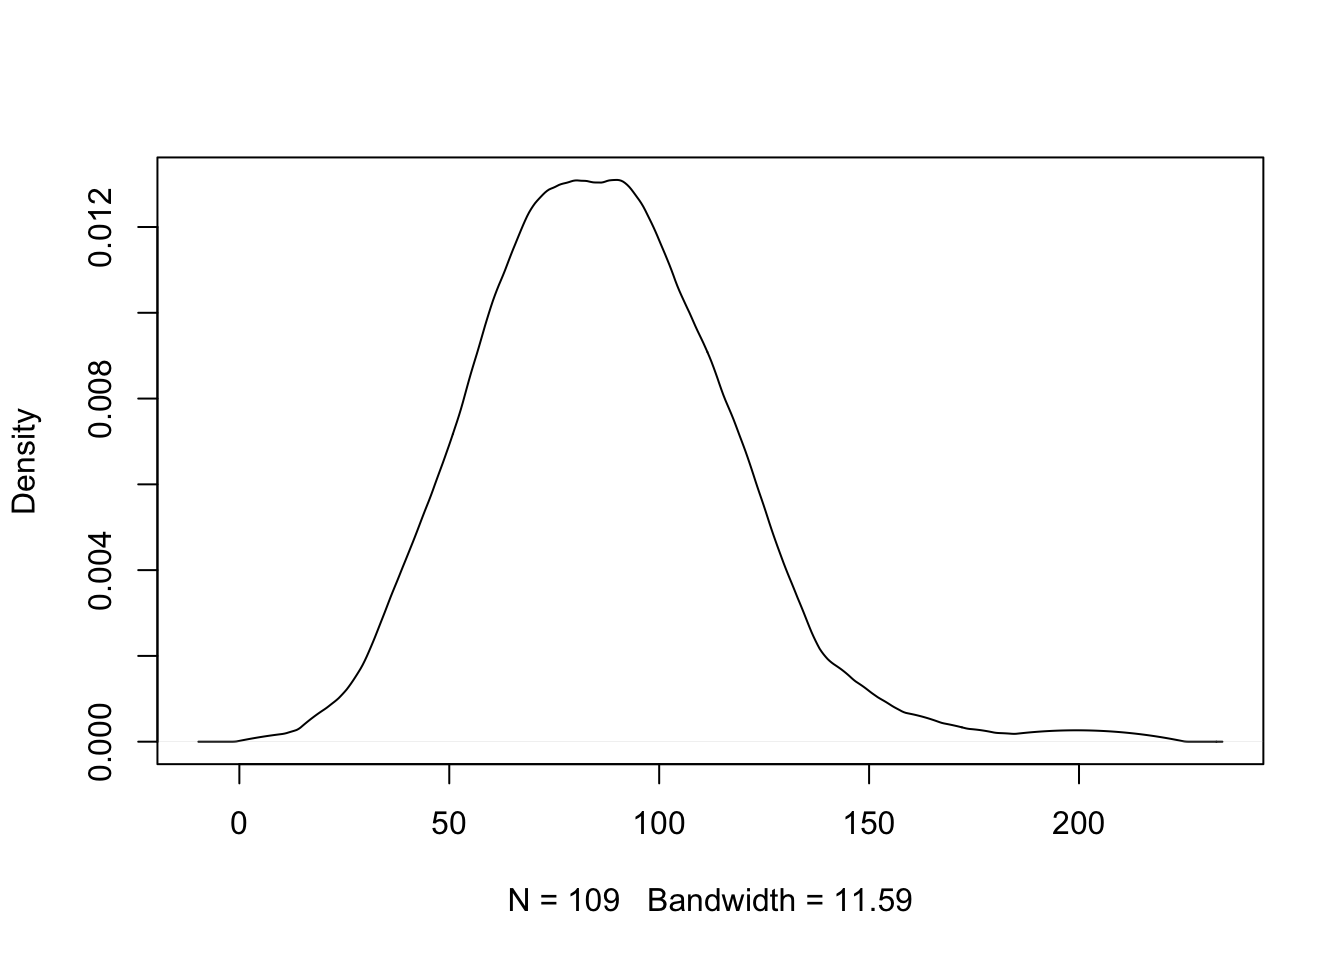
\includegraphics{MATH5714M_files/figure-latex/buffalo-final-1.pdf}

In practice one would just use one of the built-in methods, for example using
\texttt{bw="SJ"} instead of estimating the bandwidth manually.

\hypertarget{higher-dimensions}{%
\subsection{Higher Dimensions}\label{higher-dimensions}}

So far we have only considered the one-dimensional case, where the samples \(x_i\)
are real numbers. In this subsection we will sketch how these methods will need
to be adjusted for the multivariate case of \(x_i = (x_{i,1}, \ldots, x_{i,p}) \in \mathbb{R}^p\).

In this setup, a \textbf{kernel} is a function \(K\colon \mathbb{R}^p\to \mathbb{R}\) such that

\begin{itemize}
\tightlist
\item
  \(\int \cdots \int K(x) \,dx_p \cdots dx_1 = 1\),
\item
  \(K(x) = K(-x)\) and
\item
  \(K(x) \geq 0\) for all \(x\in \mathbb{R}\),
\end{itemize}

where the integral in the first condition is now over all \(p\) coordinates.

\begin{example}
If \(K_1, \ldots, K_p\) are one-dimensional kernels, then the product
\begin{equation*}
  K(x_1, \ldots, x_p)
  := K_1(x_1) \cdots K_p(x_p)
\end{equation*}
is a kernel in \(p\) dimensions. If we use the product of \(p\)
Gaussian kernels, we get
\begin{align*}
  K(x)
  &= \prod_{i=1}^p \frac{1}{\sqrt{2\pi}} \exp\bigl(-x_i^2/2\bigr) \\
  &=  \frac{1}{(2\pi)^{p/2}} \exp\Bigl(-\frac12 (x_1^2 + \cdots + x_p^2) \Bigr).
\end{align*}
\end{example}

There are different possibilities for rescaling these kernels:

\begin{itemize}
\item
  If all coordinates live on ``comparable scales'' (e.g., if they are
  measured in the same units), the formula
  \[ K_h(x) = \frac{1}{h^p} K(x/h) \]
  for all \(x\in\mathbb{R}^p\) can be used, where \(h>0\) is a bandwidth parameter
  as before. The scaling by \(1/h^p\) is required
  to ensure that the integral of \(K_h\) equals \(1\), so that \(K_h\) is
  a kernel again.
\item
  If different scaling is desirable for different components, the formula
  \begin{equation*}
    K_h(x)
    = \frac{1}{h_1 \cdots h_p} K(x_1/h_1, \ldots, x_p/h_p)
  \end{equation*}
  for all \(x\in\mathbb{R}^p\) can be used, where \(h = (h_1, \ldots, h_p)\) is a vector
  of bandwidth parameters.
\item
  A more general version would be to use a symmetric, positive definite
  bandwidth matrix \(H \in \mathbb{R}^{p\times p}\).
  In this case the required scaling is
  \begin{equation*}
    K_H(x)
    = \frac{1}{\mathrm{det}(H)} K\bigl( H^{-1} x \bigr)
  \end{equation*}
  for all \(x\in\mathbb{R}^p\).
\end{itemize}

For all of these choices, the kernel density estimator is given by
\begin{equation*}
  \hat f_h(x)
  = \frac{1}{n} \sum_{i=1}^n K_h(x - x_i)
\end{equation*}
(using \(K_H\) for the third option) for all \(x\in\mathbb{R}^p\).
Bandwidth selection in the multivariate case is a difficult problem
and we will not discuss this here.

\clearpage

\hypertarget{X05-smoothing}{%
\section{Kernel Smoothing}\label{X05-smoothing}}

We now consider the statistical model
\begin{equation*}
  Y_i
  = m(x_i) + \varepsilon_i,
\end{equation*}
where \(m\colon \mathbb{R}\to \mathbb{R}\) is a smooth function and \(\varepsilon_i\) are independent
random variables with \(\mathbb{E}(\varepsilon_i) = 0\). We are given data \((x_i, y_i)\) for
\(i\in \{1, \ldots, n\}\) and our aim is to estimate the function~\(m\). The
task of estimating the function~\(m\) from data is called \textbf{smoothing}.

\hypertarget{the-nadaraya-watson-estimator}{%
\subsection{The Nadaraya-Watson Estimator}\label{the-nadaraya-watson-estimator}}

Since we have
\begin{equation*}
  \mathbb{E}(Y_i)
  = \mathbb{E}\bigl( m(x_i) + \varepsilon_i \bigr)
  = m(x_i) + \mathbb{E}( \varepsilon_i )
  = m(x_i),
\end{equation*}
we could attempt to use a Monte-Carlo approach where we estimate the
expectation \(\mathbb{E}(Y_i)\) using an average of many \(Y\) values. This approach is
not feasible in practice, since typically we will only have \emph{a single}
observation \(y_i\) corresponding to a given \(x_i\). The idea of the
Nadaraya-Watson Estimator is to average the \(y_i\) corresponding to nearby \(x_i\)
instead. A weighted average is used, which gives less weight to further away
values. This leads to the following definition.

\begin{definition}
\protect\hypertarget{def:NW}{}\label{def:NW}The \textbf{Nadaraya-Watson Estimator} for \(m(x)\) is given by
\begin{equation*}
  \hat m_h(x)
  = \frac{\sum_{i=1}^n K_h(x - x_i) y_i}{\sum_{j=1}^n K_h(x - x_j)},
\end{equation*}
where \(K_h\) is a kernel scaled to bandwidth~\(h\) as in
definition~\ref{def:KDE}.
\end{definition}

The proble of finding \(m\) using kernel functions are called \textbf{kernel smoothing}
or \textbf{kernel regression}. In this context, the bandwidth \(h\) is also called
the \textbf{smoothing parameter}. The Nadaraya-Watson Estimator is not the only
method for kernel smoothing. We will learn about different methods in the
next sections.

Using the shorthand
\begin{equation*}
  w_i(x)
  := \frac{K_h(x - x_i)}{\sum_{j=1}^n K_h(x - x_j)}
\end{equation*}
we can write the Nadaraya-Watson Estimator as
\(\hat m_h(x) = \sum_{i=1}^n w_i(x) y_i\) and since
\begin{align*}
  \sum_{i=1}^n w_i(x)
  &= \sum_{i=1}^n \frac{K_h(x - x_i)}{\sum_{j=1}^n K_h(x - x_j)} \\
  &= \frac{\sum_{i=1}^n K_h(x - x_i)}{\sum_{j=1}^n K_h(x - x_j)} \\
  &= 1,
\end{align*}
this is indeed a weighted average.

\begin{example}
\protect\hypertarget{exm:faithful}{}\label{exm:faithful}The \texttt{faithful} dataset built into R contains 272 observations of
waiting time between eruptions and the duration of the eruption for the Old Faithful geyser in Yellowstone National Park. We can use the
\texttt{ksmooth()} function to compute Nadaraya-Watson estimate for the
waiting time after an eruption of a given length. Here we use
a Gaussian kernel with bandwidth~1.

\begin{Shaded}
\begin{Highlighting}[]
\NormalTok{x }\OtherTok{\textless{}{-}}\NormalTok{ faithful}\SpecialCharTok{$}\NormalTok{eruptions}
\NormalTok{y }\OtherTok{\textless{}{-}}\NormalTok{ faithful}\SpecialCharTok{$}\NormalTok{waiting}
\FunctionTok{plot}\NormalTok{(x, y, }\AttributeTok{cex =}\NormalTok{ .}\DecValTok{5}\NormalTok{,}
     \AttributeTok{xlab =} \StringTok{"eruption time [mins]"}\NormalTok{, }\AttributeTok{ylab =} \StringTok{"time to next eruption [mins]"}\NormalTok{)}
\FunctionTok{lines}\NormalTok{(}\FunctionTok{ksmooth}\NormalTok{(x, y, }\AttributeTok{kernel =} \StringTok{"normal"}\NormalTok{, }\AttributeTok{bandwidth =} \DecValTok{1}\NormalTok{, }\AttributeTok{n.points =} \DecValTok{1000}\NormalTok{),}
      \AttributeTok{col =} \StringTok{"red"}\NormalTok{)}
\end{Highlighting}
\end{Shaded}

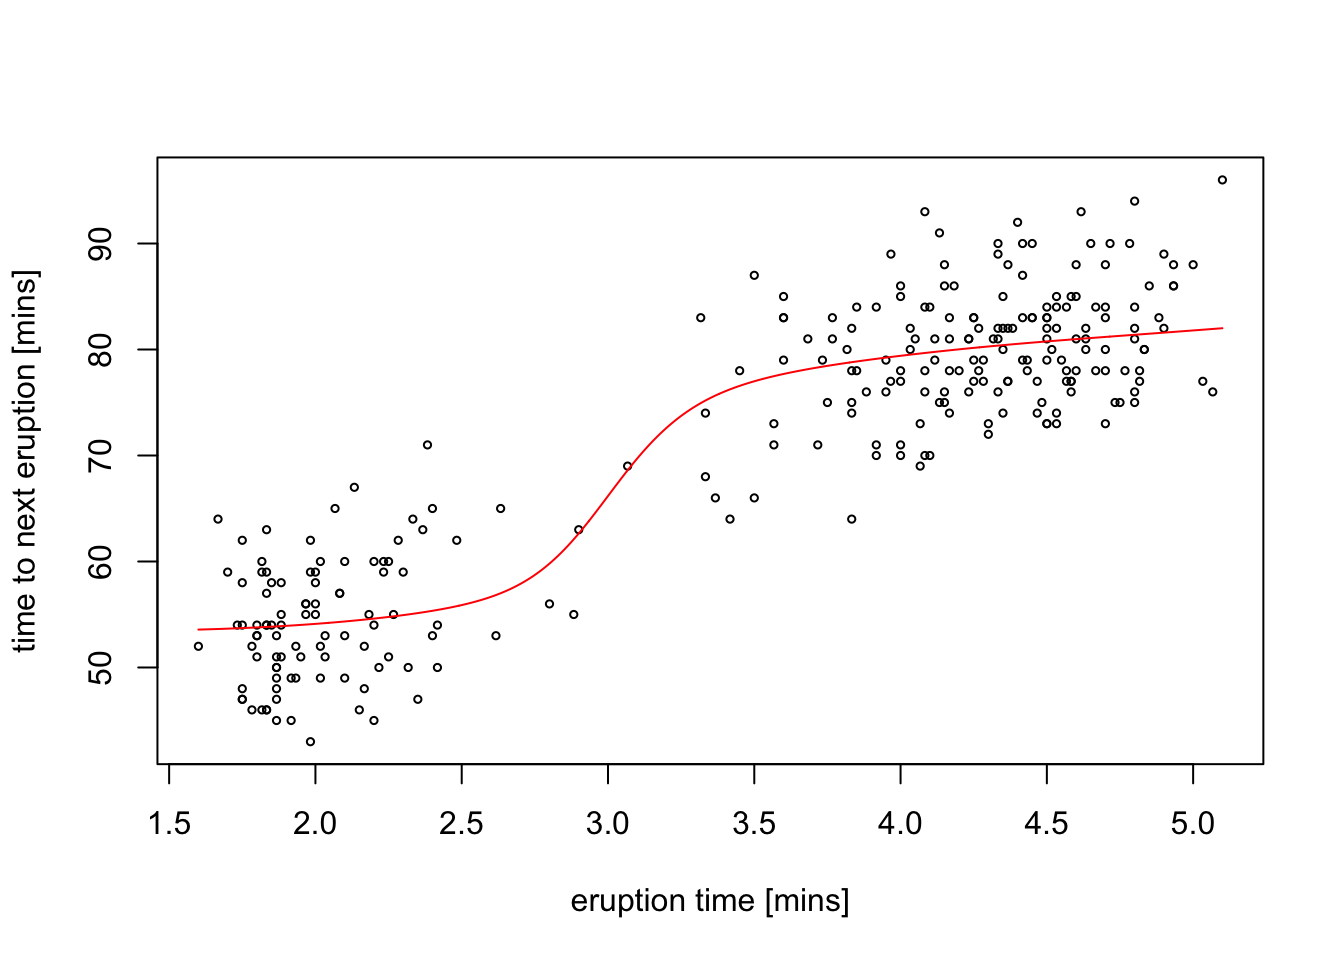
\includegraphics{MATH5714M_files/figure-latex/faithful2-1.pdf}

The estimate \(\hat m_h\) (red line) smoothly connects the two clusters
visible in the scatter plot.
\end{example}

For kernels with bounded support, \emph{e.g.}~for the Epanechnikov kernel,
the denominator \(\sum_{j=1}^n K_h(x - x_j)\) will equal zero for \(x\)
which are too far away from all of the \(x_i\). For these \(x\), the weights
\(w_i\) and thus also the estimate \(\hat m_h(x)\) are undefined. This
problem can easily be seen in practice, when the bandwidth is chosen
too small.

\begin{example}
\protect\hypertarget{exm:faithless}{}\label{exm:faithless}To illustrate the problem of the estimate becoming undefined far away
from the data points, we redo the previous estimate using a uniform
kernel:

\begin{Shaded}
\begin{Highlighting}[]
\FunctionTok{plot}\NormalTok{(x, y, }\AttributeTok{cex =}\NormalTok{ .}\DecValTok{5}\NormalTok{,}
     \AttributeTok{xlab =} \StringTok{"eruption time [mins]"}\NormalTok{, }\AttributeTok{ylab =} \StringTok{"time to next eruption [mins]"}\NormalTok{)}
\FunctionTok{lines}\NormalTok{(}\FunctionTok{ksmooth}\NormalTok{(x, y, }\AttributeTok{kernel =} \StringTok{"box"}\NormalTok{, }\AttributeTok{bandwidth =} \DecValTok{1}\NormalTok{, }\AttributeTok{n.points =} \DecValTok{1000}\NormalTok{),}
      \AttributeTok{col =} \StringTok{"red"}\NormalTok{)}
\FunctionTok{lines}\NormalTok{(}\FunctionTok{ksmooth}\NormalTok{(x, y, }\AttributeTok{kernel =} \StringTok{"box"}\NormalTok{, }\AttributeTok{bandwidth =} \FloatTok{0.1}\NormalTok{, }\AttributeTok{n.points =} \DecValTok{1000}\NormalTok{),}
      \AttributeTok{col =} \StringTok{"blue"}\NormalTok{)}
\end{Highlighting}
\end{Shaded}

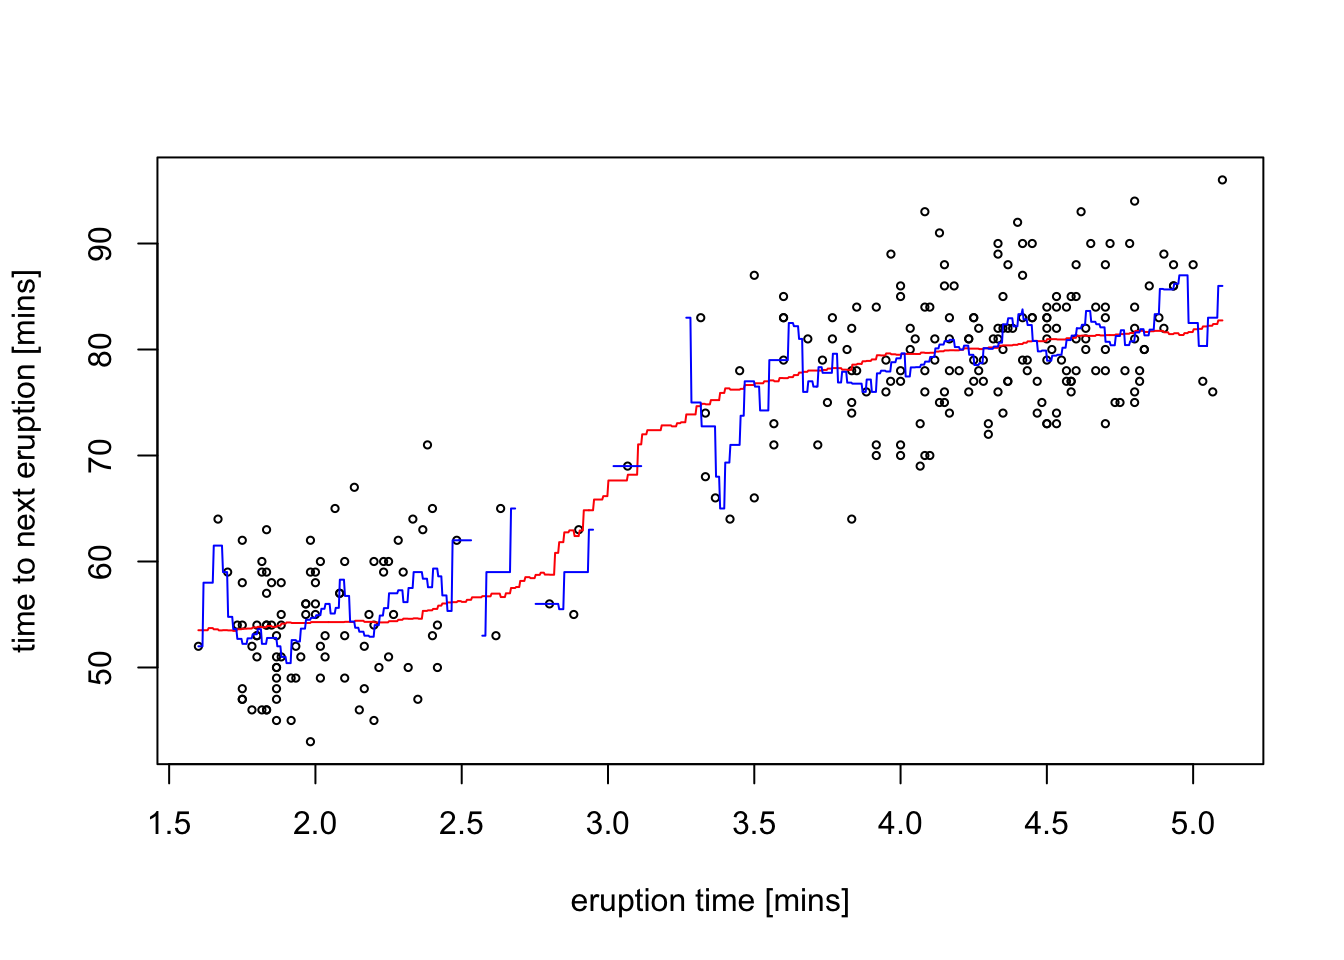
\includegraphics{MATH5714M_files/figure-latex/faithful1-1.pdf}

For \(h = 1\) (red line) we get a line \(\hat m_h\) which is less smooth than
the estimate using the Gaussian kernel, but is otherwise looks similar to
the previous estimate. In contrast, if we reduce the bandwidth to \(h = 0.1\)
(blue line), gaps start to appear in the plot of \(\hat m_h\) where the
spacing of the data points is too large.
\end{example}

\hypertarget{estimation-error}{%
\subsection{Estimation Error}\label{estimation-error}}

Here we will discuss how fast the estimation error decreases in the
limit of \(n\to \infty\), \emph{i.e.}~for the case when we have a large dateset
to use for the estimate. As before, we will find that we need to decrease
the bandwidth \(h\) as \(n\) increases.

To allow for \(n\) to change, we will introduce a statistical model
also for the inputs \(x_i\). (This is different from what we did
in the level 3 part of the module for linear regression.) Here
we will consider the following model:

\begin{itemize}
\tightlist
\item
  \(X_1, \ldots, X_n\) are independent and identically distributed with
  density~\(f\).
\item
  \(\eta_1, \ldots \eta_n\) are independent, with \(\mathbb{E}(\eta_i) = 0\)
  and \(\mathop{\mathrm{Var}}(\eta_i) = 1\).
\item
  \(\varepsilon_i = s(X_i) \eta_i\) for all \(i \in \{1, \ldots, n\}\),
  where \(s\colon \mathbb{R}\to (0, \infty)\) is a smooth function.
\item
  \(Y_i = m(X_i) + \varepsilon_i\) where \(m\colon \mathbb{R}\to \mathbb{R}\) is a smooth function.
\end{itemize}

While this extended model allows us to increase \(n\), it also creates
a practical problem: the estimator
\begin{equation*}
  \hat m_h(x)
  = \frac{\sum_{i=1}^n K_h(x - X_i) Y_i}{\sum_{j=1}^n K_h(x - X_j)},
\end{equation*}
now has random terms both in the numerator and in the denominator.
This will make it more challenging to determine the behaviour
of \(\mathbb{E}\bigl( \hat m_h(x) \bigr)\) and \(\mathop{\mathrm{Var}}\bigl( \hat m_h(x) \bigr)\)
as \(n \to \infty\) and \(h \downarrow 0\). We can write \(\hat m_h(x)\) as
\begin{equation}
  \hat m_h(x)
  = \frac{\frac1n \sum_{i=1}^n K_h(x - X_i) Y_i}{\frac1n \sum_{j=1}^n K_h(x - X_j)}
  = \frac{\frac1n \sum_{i=1}^n K_h(x - X_i) Y_i}{\hat f_h(x)}
  = \frac{\hat r_h(x)}{\hat f_h(x)}  \label{eq:m-hat-h}
\end{equation}
where \(\hat f_h(x)\) is the kernel density estimator from
\protect\hyperlink{X01-KDE}{Section 1} and
\begin{equation*}
  \hat r_h(x)
  := \frac1n \sum_{i=1}^n K_h(x - X_i) Y_i.
\end{equation*}
We will consider the numerator and denominator of equation \eqref{eq:m-hat-h}
separately

\hypertarget{denominator}{%
\subsubsection*{Denominator}\label{denominator}}
\addcontentsline{toc}{subsubsection}{Denominator}

From equations \eqref{eq:fhatbias} and \eqref{eq:fhatvar} we know that
\begin{equation*}
  \mathbb{E}\bigl( \hat f_h(x) \bigr)
  \approx f(x) + \frac{\mu_2(K) f''(x)}{2} h^2
\end{equation*}
and
\begin{equation*}
  \mathop{\mathrm{Var}}\bigl( \hat f_h(x) \bigr)
  \approx \frac{1}{nh} f(x) R(K)
\end{equation*}
as \(h \downarrow 0\).

\hypertarget{numerator}{%
\subsubsection*{Numerator}\label{numerator}}
\addcontentsline{toc}{subsubsection}{Numerator}

We start by considering the numerator \(\hat r_h(x)\). The arguments used here
will be very similar to the arguments used in the section about the
\protect\hyperlink{X03-Var}{variance of kernel density estimates}.

The expectation of \(\hat r_h(x)\) is
\begin{align*}
  \mathbb{E}\bigl( \hat r_h(x) \bigr)
  &= \mathbb{E}\Bigl( \frac1n \sum_{i=1}^n K_h(x - X_i) Y_i \Bigr) \\
  &= \frac1n \sum_{i=1}^n \mathbb{E}\bigl( K_h(x - X_i) Y_i \bigr) \\
  &= \mathbb{E}\bigl( K_h(x - X) Y \bigr) \\
  &= \mathbb{E}\Bigl( K_h(x - X) (m(X) + \sigma(X)\eta) \Bigr).
\end{align*}
We use integrals to average over the randomness in \(X\) and \(\eta\),
denoting the density of \(\eta\) by~\(\varphi\):
\begin{align*}
  \mathbb{E}\bigl( \hat r_h(x) \bigr)
  &= \int \int K_h(x - \xi) \bigl( m(\xi) + \sigma(\xi) e \bigr) \, \varphi(e) \, de \, f(\xi) \, d\xi \\
  &= \int K_h(x - \xi) \Bigl( m(\xi) +\sigma(\xi) \int e \, \varphi(e) \, de \Bigr) \, f(\xi) \, d\xi \\
  &= \int K_h(x - \xi) m(\xi) f(\xi) \, d\xi,
\end{align*}
since
\begin{equation*}
  \int e \, \varphi(e) \, de
  = \mathbb{E}(\eta)
  = 0.
\end{equation*}
Writing
\begin{equation*}
  r(x)
  := m(x) f(x)
\end{equation*}
as an abbreviation, we finally get
\begin{equation*}
  \mathbb{E}\bigl( \hat r_h(x) \bigr)
  = \int K_h(x - \xi) r(\xi) \, d\xi.
\end{equation*}

We now formalise an argument which we already used earlier.

\begin{lemma}
\protect\hypertarget{lem:kernel-limit}{}\label{lem:kernel-limit}

Let \(g\colon \mathbb{R}\to \mathbb{R}\) be two times continuously differentiable
and let \(K\) be a kernel function. Then we have

\begin{enumerate}
\def\labelenumi{\arabic{enumi}.}
\tightlist
\item
  \(\displaystyle\int K_h(x - \xi) g(\xi) \, d\xi = g(x) + \frac12 \mu_2(K) g''(x) h^2 + o(h^2)\)
  as \(h \downarrow 0\), and
\item
  \(\displaystyle\int K_h(x - \xi)^2 g(\xi) \, d\xi = \frac1h R(K) g(x) + o(1/h)\)
  as \(h \downarrow 0\).
\end{enumerate}

\end{lemma}

\begin{proof}
The first statement is proved using substitution and Taylor expandion of \(r\)
around \(x\) as shown in the derivation of equation~\eqref{eq:fhatbias}.
The second statement is proved similarly, as shown in the derivation of
equation~\eqref{eq:Var-frag1}.
\end{proof}

Using the first part of lemma~\ref{lem:kernel-limit} for \(g = r\) we get
\begin{equation*}
  \mathbb{E}\bigl( \hat r_h(x) \bigr)
  = r(x) + \frac12 \mu_2(K) r''(x) h^2 + o(h^2).
\end{equation*}

For the variance of \(\hat r_h(x)\) we get
\begin{align*}
  \mathop{\mathrm{Var}}\bigl( \hat r_h(x) \bigr)
  &= \mathop{\mathrm{Var}}\Bigl( \frac1n \sum_{i=1}^n K_h(x - X_i) Y_i \Bigr) \\
  &= \frac{1}{n^2} \sum_{i=1}^n \mathop{\mathrm{Var}}\bigl( K_h(x - X_i) Y_i \bigr) \\
  &= \frac1n \mathop{\mathrm{Var}}\bigl( K_h(x - X) Y \bigr) \\
  &= \frac1n \Bigl( \mathbb{E}\bigl( K_h(x - X)^2 Y^2 \bigr) - \mathbb{E}\bigl( K_h(x - X) Y \bigr)^2 \Bigr).
\end{align*}
We have already seen that
\begin{equation*}
  \mathbb{E}\bigl( K_h(x - X) Y \bigr)
  = \mathbb{E}\bigl( \hat r_h(x) \bigr)
  = r(x) + \frac12 \mu_2(K) r''(x) h^2 + o(h^2)
\end{equation*}
and thus
\begin{equation*}
  \mathbb{E}\bigl( K_h(x - X) Y \bigr)^2
  = r(x)^2 + O(h^2).
\end{equation*}
Using the second part of lemma~\ref{lem:kernel-limit} one can show that
\begin{align*}
  \mathbb{E}\bigl( K_h(x - X)^2 Y^2 \bigr)
  &= \int \int K_h(x - \xi)^2 \bigl( m(\xi) + s(\xi)e \bigr)^2 \,\varphi(e)\,de \,f(\xi)\,d\xi \\
  &= \int K_h(x - \xi)^2 \bigl( m(\xi)^2 + s(\xi)^2 \bigr) f(\xi) \,d\xi \\
  &= \frac1h R(K) \bigl( m(x)^2 + s(x)^2 \bigr) f(x) + o(1/h).
\end{align*}
Combining these equations we find
\begin{equation*}
  \mathop{\mathrm{Var}}\bigl( \hat r_h(x) \bigr)
  \approx \frac{1}{nh} R(K) \bigl( m(x)^2 + s(x)^2 \bigr) f(x)
    + \frac1n r(x)^2
\end{equation*}
as \(n\to\infty\), \(h\downarrow 0\) and \(nh\to\infty\).

\hypertarget{mean-squared-error-1}{%
\subsubsection*{Mean Squared Error}\label{mean-squared-error-1}}
\addcontentsline{toc}{subsubsection}{Mean Squared Error}

To turn our results about \(\hat r_h\) and our previous results about
\(\hat f\) into an error estimate for
\begin{equation*}
  \hat m_h(x)
  = \frac{\hat r_h(x)}{\hat f_h(x)},
\end{equation*}
we consider Taylor expansion of the function \(g(y) = 1/y\):
\begin{align*}
  g(y + h)
  &= g(y) + g'(y) h + o(h) \\
  &= \frac1y - \frac{1}{y^2} h + o(h).
\end{align*}
Using this approximation we get
\begin{align*}
  \hat m_h(x)
  &= \hat r_h(x) g\bigl( \hat f_h(x) \bigr) \\
  &= \hat r_h(x) g\bigl( f(x) + \hat f_h(x) - f(x) \bigr) \\
  &\approx \hat r_h(x) \Bigl( \frac{1}{f(x)} - \frac{1}{f(x)^2} (\hat f_h(x) - f(x)) \Bigr) \\
  &= \frac{\hat r_h(x)}{f(x)} - \frac{\hat r_h(x) \bigl(\hat f_h(x) - f(x) \bigr)}{f(x)^2}.
\end{align*}
With the help of this trick, we have achieved that now all random terms
are in the denominator and thus we can take expectations easily:
\begin{align*}
  \mathbb{E}\bigl( \hat m_h(x) \bigr)
  &= \frac{\mathbb{E}\bigl( \hat r_h(x) \bigr)}{f(x)}
      - \frac{\mathbb{E}\Bigl( \hat r_h(x) \bigl(\hat f_h(x) - f(x) \bigr) \Bigr)}{f(x)^2} \\
  &\approx \frac{\mathbb{E}\bigl( \hat r_h(x) \bigr)}{f(x)}
      - \frac{\mathbb{E}\bigl( \hat r_h(x) \bigr) \mathbb{E}\bigl( \hat f_h(x) - f(x) \bigr)}{f(x)^2}.
\end{align*}
Substituting in our previous results we get
\begin{align*}
  \mathbb{E}\bigl( \hat m_h(x) \bigr)
  &\approx \frac{r(x) + \frac12 \mu_2(K) r''(x) h^2 + o(h^2)}{f(x)}
      - \frac{\bigl( r(x) + \frac12 \mu_2(K) r''(x) h^2 + o(h^2) \bigr)
          \frac12 \mu_2(K) f''(x) h^2}{f(x)^2} \\
  &= \frac{r(x)}{f(x)}
    + \frac12 \frac{\mu_2(K) r''(x)}{f(x)} h^2
    - \frac12 \frac{\mu_2(x) r(x) f''(x)}{f(x)^2} h^2
    + o(h^2)
\end{align*}
Using \(r(x) = f(x) m(x)\) we find the derivative
\(r'(x) = f'(x) m(x) + f(x) m'(x)\)
as well as the second derivative
\(r''(x) = f''(x) m(x) + 2 f'(x) m'(x) + f(x) m''(x)\).
This gives
\begin{align*}
  \mathbb{E}\bigl( \hat m_h(x) \bigr)
  &= m(x)
    + \frac12 \frac{\mu_2(K) r''(x)}{f(x)} h^2
    - \frac12 \frac{\mu_2(x) m(x) f''(x)}{f(x)} h^2
    + o(h^2) \\
  &= m(x)
    + \frac12 \frac{\mu_2(K) \bigl(2 f'(x) m'(x) + f(x) m''(x)\bigr)}{f(x)} h^2
    + o(h^2) \\
  &= m(x)
    + \mu_2(K) \Bigl( \frac{f'(x)}{f(x)} m'(x) + \frac12 m''(x) \Bigr) h^2
    + o(h^2)
\end{align*}
and
\begin{equation*}
  \mathop{\mathrm{bias}}\bigl( \hat m_h(x) \bigr)
  = \mu_2(K) \Bigl( \frac{f'(x)}{f(x)} m'(x) + \frac12 m''(x) \Bigr) h^2
    + o(h^2).
\end{equation*}

A similar calculation gives the approximate variance as
\begin{equation*}
  \mathop{\mathrm{Var}}\bigl( \hat m_h(x) \bigr)
  = \frac{1}{nh} \frac{\sigma^2(x) R(K)}{f(x)} + o\Bigl( \frac{1}{nh} \Bigr).
\end{equation*}
So finally we have
\begin{align*}
  \mathop{\mathrm{MSE}}\nolimits\bigl( \hat m_h(x) \bigr)
  &= \frac{h^4 \mu_2(K)^2}{4} \Bigl(m''(x) +\frac{2m'(x) f'(x)}{f(x)} \Bigr)^2 \\
  &\hskip1cm + \frac{1}{nh} \frac{\sigma^2(x) R(K)}{f(x)} + o\Bigl( \frac{1}{nh} \Bigr) + o(h^4).
\end{align*}

\textbf{Notes:}

\begin{itemize}
\tightlist
\item
  A more careful calculation will need to take into account that \(\hat m(x)\)
  may be undefined. All expectations and variances are conditional on
  \(\hat f(x) \neq 0\). One can show that \(P\bigl( \hat f(x) \neq 0 \bigr) \to 1\)
  as \(n\to\infty\) for all \(x\in\mathbb{R}\) with \(f(x) > 0\), so this is not a problem.
\item
  The MSE is of order \(O(n^{-4/5})\) when we choose \(h \sim n^{-1/5}\), as before.
\item
  The formula for the variance shows that the regression curve is more stable
  in those areas where there are plenty of observations.
\item
  The bias-squared is either dominated by the second derivative
  \(m''(x)\) - when we are close to a local extremum of \(m(x)\) (turning point),
  or by the first derivative \(m'(x)\) when we have few observations.
\item
  This calculation is helpful in creating confidence intervals for the estimate
  \(\hat m_h(x)\) in which \(\sigma^2(x)\) can be estimated by
  \[\hat \sigma^2(x) = \sum w_i(x) \bigl( y_i-\hat m_h^{(i)}(x_i) \bigr)^2,\]
  where \(\hat m_h^{(i)}(x_i)\) is the estimate of \(m\) at the point \(x_i\) using
  all of the data except for the observation at \((x_i, y_i)\).
\end{itemize}

\textbf{Summary}

\begin{itemize}
\tightlist
\item
  We have learned how the Nadaraya-Watson Estimator can be used
  for smoothing.
\item
  We have considered the mean squared error of this estimator.
\end{itemize}

\clearpage

\hypertarget{X06-locpoly}{%
\section{Local Polynomial Regression}\label{X06-locpoly}}

Local polynomial regression is a generalisation of the
Nadaraya-Watson estimator. The method combines the two ideas of
linear regression with weights and polynomial regression. The aim
is still to estimate the model mean \(m \colon\mathbb{R}\to \mathbb{R}\) from
given data \((x_1, y_1), \ldots, (x_n, y_n)\).

\hypertarget{linear-regression-with-weights}{%
\subsection{Linear Regression with Weights}\label{linear-regression-with-weights}}

In the \href{https://seehuhn.github.io/MATH3714/S02-multiple.html\#the-normal-equations}{level 3 part of the module},
we introduced the least squares method for linear regression. This method
estimartes the regression coefficients by minimising the residual sum of
squares:
\begin{align*}
  r(\beta)
  &= \sum_{i=1}^n \hat\varepsilon_i^2 \\
  &= \hat\varepsilon^\top \hat\varepsilon.
\end{align*}
Here we will extend this method to include weights for the observations.
Given weights
\(w_1, \ldots, w_n > 0\), the weighted least squares method minimises
\begin{equation*}
  r_w(\beta)
  = \sum_{i=1}^n w_i \varepsilon_i^2.
\end{equation*}
In matrix notation, this function can be written as
\begin{align*}
  r_w(\beta)
  = \varepsilon^\top W \varepsilon
  = (y - X \beta)^\top W (y - X \beta),
\end{align*}
where \(W\) is a diagonal matrix with the weights on the diagonal:
\begin{equation}
  W
  = \begin{pmatrix}
      w_1 & 0 & 0 & \cdots & 0 \\
      0 & w_2 & 0 & \cdots & 0 \\
      0 & 0 & w_3 & \cdots & 0 \\
      \vdots & \vdots & \vdots & \ddots & \vdots \\
      0 & 0 & 0 & \cdots & w_n
    \end{pmatrix}.  \label{eq:W-diagonal}
\end{equation}
Similar to \href{https://seehuhn.github.io/MATH3714/S02-multiple.html\#lem:multiple-LSQ}{lemma 2.1 in the level 3 notes},
we can take derivatives to find
the minimum of~\(r_w\). The result is
\begin{equation*}
  \hat\beta
  = (X^\top W X)^{-1} X^\top W y.
\end{equation*}

Since \(W\) appears once in the inverse and once before the \(y\), we can
multiply \(W\) by any number without changing the result. Thus we don't
need to ``normalise'' the weights \(w_i\) to sum to one.

As before, the fitted value for inputs \((\tilde x_1, \ldots, \tilde x_p) \in \mathbb{R}^p\) is given by
\begin{equation*}
  \hat\beta_0 + \hat\beta_1 \tilde x_1 + \cdots + \hat\beta_p \tilde x_p
  = \tilde x^\top \hat\beta,
\end{equation*}
where \(\tilde x = (1, \tilde x_1, \ldots, \tilde x_n)\).

\hypertarget{polynomial-regression}{%
\subsection{Polynomial Regression}\label{polynomial-regression}}

In these notes we only consider the case of \(p=1\). In this case we
can easily fit a polynomial of degree \(p\) to the data by using
\(x, x^2, \ldots, x^p\) as the input variables. The corresponding
model is
\begin{equation*}
  y
  = \beta_0 + \beta_1 x + \beta_2 x^2 + \cdots + \beta_p x^p + \varepsilon.
\end{equation*}
This leads to the design matrix
\begin{equation*}
  X
  = \begin{pmatrix}
      1 & x_1 & x_1^2 & \cdots & x_1^p \\
      1 & x_2 & x_2^2 & \cdots & x_2^p \\
      \vdots & \vdots & \vdots & \ddots & \vdots \\
      1 & x_n & x_n^2 & \cdots & x_n^p
    \end{pmatrix}.
\end{equation*}

\begin{example}
To illustrate polynomial regression, we fit a third-order polynomial
to a simple, simulated dataset. Since the operator \texttt{\^{}} has a special
meaning inside \texttt{lm()}, we have to use the function \texttt{I()} (which disables
the special meaning of \texttt{+} and \texttt{\^{}} for its arguments) when computing
the inputs \(x^2\) and~\(x^3\).

\begin{Shaded}
\begin{Highlighting}[]
\FunctionTok{set.seed}\NormalTok{(}\DecValTok{20211102}\NormalTok{)}

\NormalTok{n }\OtherTok{\textless{}{-}} \DecValTok{40}
\NormalTok{x }\OtherTok{\textless{}{-}} \FunctionTok{seq}\NormalTok{(}\DecValTok{0}\NormalTok{, }\DecValTok{10}\NormalTok{, }\AttributeTok{length.out =}\NormalTok{ n)}
\NormalTok{y }\OtherTok{\textless{}{-}} \FunctionTok{cos}\NormalTok{(x) }\SpecialCharTok{+} \FunctionTok{rnorm}\NormalTok{(n, }\AttributeTok{sd =} \FloatTok{0.5}\NormalTok{)}

\NormalTok{m }\OtherTok{\textless{}{-}} \FunctionTok{lm}\NormalTok{(y }\SpecialCharTok{\textasciitilde{}}\NormalTok{ x }\SpecialCharTok{+} \FunctionTok{I}\NormalTok{(x}\SpecialCharTok{\^{}}\DecValTok{2}\NormalTok{) }\SpecialCharTok{+} \FunctionTok{I}\NormalTok{(x}\SpecialCharTok{\^{}}\DecValTok{3}\NormalTok{))}

\FunctionTok{plot}\NormalTok{(x, y)}
\FunctionTok{lines}\NormalTok{(x, }\FunctionTok{fitted}\NormalTok{(m))}
\end{Highlighting}
\end{Shaded}

\includegraphics{MATH5714M_files/figure-latex/polreg1-1.pdf}

The resulting regression line seems like a resonable fit for the data.
We note that a third-order polynomial grows very quickly to \(\pm\infty\)
as \(|x|\) increases. Thus, the fitted model cannot be used for extrapolating
beyond the range of the data.
\end{example}

When the regression is set up in this way, the design matrix often suffers
from collinearity. To check for this, we can consider the condition
number~\(\kappa\). For the example above we get the following value:

\begin{Shaded}
\begin{Highlighting}[]
\FunctionTok{kappa}\NormalTok{(m)}
\end{Highlighting}
\end{Shaded}

\begin{verbatim}
## [1] 2813.242
\end{verbatim}

This is a large value, indicating collinearity. To improve the setup
of the problem we can use the model
\begin{equation*}
  y
  = \beta_0 + \beta_1 (x - \tilde x) + \beta_2 (x - \tilde x)^2 + \cdots + \beta_p (x - \tilde x)^p + \varepsilon,
\end{equation*}
where \(\tilde x\) is inside the interval if \(x\) values.
This leads to the design matrix
\begin{equation}
  X
  = \begin{pmatrix}
      1 & (x_1-\tilde x) & (x_1-\tilde x)^2 & \cdots & (x_1-\tilde x)^p \\
      1 & (x_2-\tilde x) & (x_2-\tilde x)^2 & \cdots & (x_2-\tilde x)^p \\
      \vdots & \vdots & \vdots & \ddots & \vdots \\
      1 & (x_n-\tilde x) & (x_n-\tilde x)^2 & \cdots & (x_n-\tilde x)^p
    \end{pmatrix}.  \label{eq:X-local}
\end{equation}

\begin{example}
Continuing from the previous example, we can see that writing the model as in\\
\eqref{eq:X-local} greatly improves the condition number:

\begin{Shaded}
\begin{Highlighting}[]
\NormalTok{x.tilde }\OtherTok{\textless{}{-}} \DecValTok{5}
\NormalTok{m2 }\OtherTok{\textless{}{-}} \FunctionTok{lm}\NormalTok{(y }\SpecialCharTok{\textasciitilde{}} \FunctionTok{I}\NormalTok{(x}\SpecialCharTok{{-}}\NormalTok{x.tilde) }\SpecialCharTok{+} \FunctionTok{I}\NormalTok{((x}\SpecialCharTok{{-}}\NormalTok{x.tilde)}\SpecialCharTok{\^{}}\DecValTok{2}\NormalTok{) }\SpecialCharTok{+} \FunctionTok{I}\NormalTok{((x}\SpecialCharTok{{-}}\NormalTok{x.tilde)}\SpecialCharTok{\^{}}\DecValTok{3}\NormalTok{))}
\FunctionTok{kappa}\NormalTok{(m2)}
\end{Highlighting}
\end{Shaded}

\begin{verbatim}
## [1] 65.75674
\end{verbatim}

While there is still collinearity, the condition number is now much smaller.
\end{example}

Polynomials of higher degree take very large values as \(|x|\) increases.
These polynomials are best used for local interpolation of data.
In contrast, polynomials of higher degree often make poor global models.

\hypertarget{polynomial-regression-with-weights}{%
\subsection{Polynomial Regression with Weights}\label{polynomial-regression-with-weights}}

The idea of local polynomial regression is to combine polynomial regression
with weights which give more weight to close by observations: to get an
estimate at a point \(\tilde x \in \mathbb{R}\), we define
\begin{equation*}
  w_i
  := K_h(\tilde x - x_i),
\end{equation*}
where \(K_h\) is a scaled kernel function as before. Using the diagonal
matrix \(W\) from~\eqref{eq:W-diagonal} for the weights and the matrix
\(X\) from~\eqref{eq:X-local} as the design matrix, we can fit a polynomial
of degree \(p\) to the data which fits the data near \(\tilde x\) well.
The regression coefficients are again estimated as
\begin{equation*}
  \hat\beta
  = (X^\top W X)^{-1} X^\top W y
\end{equation*}
and the model mean near \(\tilde x\) is given by
\begin{equation*}
  \hat m_h(x; \tilde x)
  = \hat\beta_0 + \hat\beta_1 (x - \tilde x) + \hat\beta_2 (x - \tilde x)^2 + \cdots + \hat\beta_p (x - \tilde x)^p,
\end{equation*}
where the weights \(\hat\beta\) depend on \(\tilde x\). The model mean at
\(x = \tilde x\) simplifies to
\begin{align*}
  \hat m_h(\tilde x)
  &= \hat m_h(\tilde x; \tilde x) \\
  &= \hat\beta_0 + \hat\beta_1 (\tilde x - \tilde x) + \hat\beta_2 (\tilde x - \tilde x)^2 + \cdots + \hat\beta_p (\tilde x - \tilde x)^p \\
  &= \hat\beta_0.
\end{align*}
Using matrix notation, we can write this as
\begin{align*}
  \hat m_h(\tilde x)
  &= \hat\beta_0 \\
  &= e_0^\top \hat\beta \\
  &= e_0^\top (X^\top W X)^{-1} X^\top W y,
\end{align*}
where \(e_0 = (1, 0, \ldots, 0) \in \mathbb{R}^{p+1}\).

Since both \(X\) and \(W\) depend on \(\tilde x\), we need to evaluate
\((X^\top W X)^{-1} X^\top W y\) separately for each \(\tilde x\) where
an estimate of \(\hat m_h\) is needed. To get a regression line, this needs
to be done over a grid of \(\tilde x\) values. Thus, this method can
be computationally expensive.

\hypertarget{special-cases}{%
\subsection{Special Cases}\label{special-cases}}

Here we discuss the special cases of \(p=0\), \(p=1\), and \(p=2\).

\hypertarget{p-0}{%
\subsubsection*{\texorpdfstring{\(p = 0\)}{p = 0}}\label{p-0}}
\addcontentsline{toc}{subsubsection}{\(p = 0\)}

For \(p=0\), the polynomial consists only of the constant term \(\beta_0\).
In this case, the design matrix \(X\) simplifies to \(X = (1, \ldots, 1) \in \mathbb{R}^{n\times 1}\). Thus we have
\begin{align*}
  X^\top W X
  &= (1, \ldots, 1)^\top W (1, \ldots, 1) \\
  &= \sum_{i=1}^n w_i \\
  &= \sum_{i=1}^n K_h(\tilde x - x_i).
\end{align*}
Similarly, we have
\begin{align*}
  X^\top W y
  &= (1, \ldots, 1)^\top W y \\
  &= \sum_{i=1}^n w_i y_i \\
  &= \sum_{i=1}^n K_h(\tilde x - x_i) y_i.
\end{align*}
Thus we find
\begin{align*}
  \hat m_h(\tilde x)
  &= (X^\top W X)^{-1} X^\top W y \\
  &= \frac{\sum_{i=1}^n K_h(\tilde x - x_i) y_i}{\sum_{i=1}^n K_h(\tilde x - x_i)}.
\end{align*}
This is the same formula as in definition~\ref{def:NW}: for \(p=0\)
the local polynomial regression estimator is the same as the Nadaraya-Watson
estimator.

\hypertarget{p-1}{%
\subsubsection*{\texorpdfstring{\(p = 1\)}{p = 1}}\label{p-1}}
\addcontentsline{toc}{subsubsection}{\(p = 1\)}

For \(p=1\) the polynomial is a straight line, allowing to model the
value as well as the slope of the mean line. The resulting estimator
is called the \emph{local linear estimator}.
This sometimes gives
a better fit than the Nadaraya-Watson estimator, for example at the boundaries
of the domain.

\begin{example}
We can use the R function \texttt{locpoly} from the \texttt{KernSmooth} package to
compute locally polynomial regression estimates. Here we plot
the estimate for \(p=1\) (blue line) together with the Nadaraya-Watson
estimator (red line), for a simple, simulated dataset.
Unfortunately, the function \texttt{locpoly()} has an interpretation of the bandwidth
which is different from what \texttt{ksmooth()} uses. Experimentally I found
that \texttt{bandwidth\ =\ 0.3} for \texttt{ksmooth()} corresponds to
\texttt{bandwidth\ =\ 0.11} for \texttt{locpoly()}: the output of
\texttt{ksmooth(...,\ bandwidth\ =\ 0.3)}
and of \texttt{locpoly(x..,\ degree\ =\ 0,\ bandwidth\ =\ 0.11)} is near identical.

\begin{Shaded}
\begin{Highlighting}[]
\FunctionTok{set.seed}\NormalTok{(}\DecValTok{20211103}\NormalTok{)}

\NormalTok{n }\OtherTok{\textless{}{-}} \DecValTok{200}
\NormalTok{x }\OtherTok{\textless{}{-}} \FunctionTok{seq}\NormalTok{(}\DecValTok{0}\NormalTok{, }\DecValTok{1}\NormalTok{, }\AttributeTok{length.out =}\NormalTok{ n)}
\NormalTok{y }\OtherTok{\textless{}{-}}\NormalTok{ x }\SpecialCharTok{+} \FunctionTok{rnorm}\NormalTok{(n, }\AttributeTok{sd =} \FloatTok{0.05}\NormalTok{)}
\FunctionTok{plot}\NormalTok{(x, y, }\AttributeTok{cex =}\NormalTok{ .}\DecValTok{5}\NormalTok{)}

\NormalTok{m1 }\OtherTok{\textless{}{-}} \FunctionTok{ksmooth}\NormalTok{(x, y, }\AttributeTok{kernel =} \StringTok{"normal"}\NormalTok{, }\AttributeTok{bandwidth =} \FloatTok{0.3}\NormalTok{)}
\FunctionTok{lines}\NormalTok{(m1, }\AttributeTok{col =} \StringTok{"red"}\NormalTok{)}

\FunctionTok{library}\NormalTok{(KernSmooth)}
\NormalTok{m2 }\OtherTok{\textless{}{-}} \FunctionTok{locpoly}\NormalTok{(x, y, }\AttributeTok{degree =} \DecValTok{1}\NormalTok{, }\AttributeTok{bandwidth =} \FloatTok{0.11}\NormalTok{)}
\FunctionTok{lines}\NormalTok{(m2, }\AttributeTok{col =} \StringTok{"blue"}\NormalTok{)}
\end{Highlighting}
\end{Shaded}

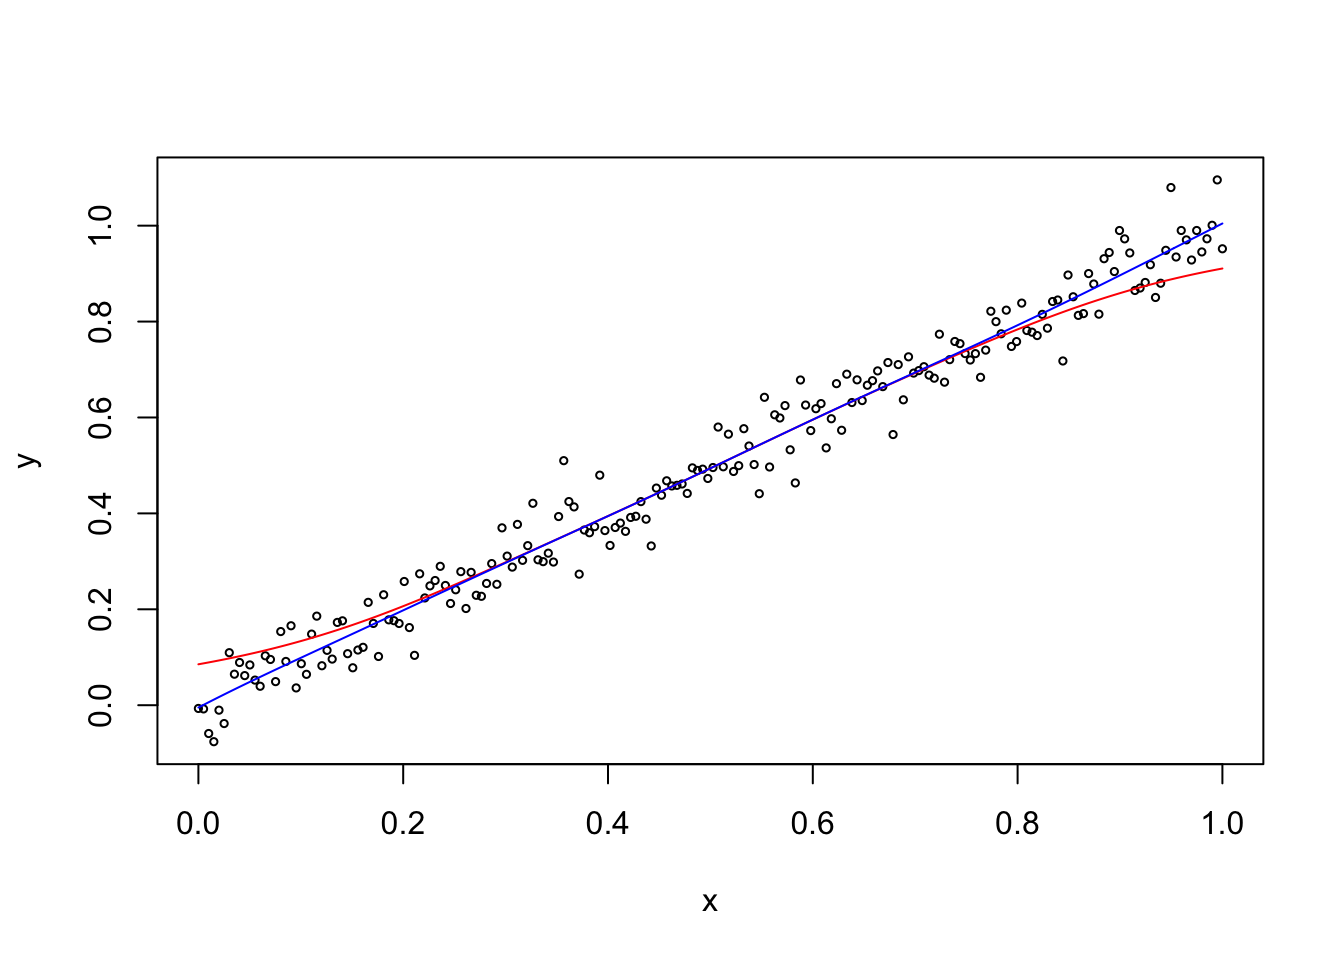
\includegraphics{MATH5714M_files/figure-latex/locpoly1-1.pdf}

Near the boundaries the Nadaray-Watson estimator is biased, because on
the left-hand boundary all nearby samples correspond to larger values of the
mean line, and similarly on the right-hand all nearby samples correspond to
smaller values of the mean line. In contrast, the local polynomial estimate
retains its slope right up to the boundary.
\end{example}

\hypertarget{p-2}{%
\subsubsection*{\texorpdfstring{\(p = 2\)}{p = 2}}\label{p-2}}
\addcontentsline{toc}{subsubsection}{\(p = 2\)}

For \(p=2\) the local polynomials are parabolas. This allows sometimes to reduce
bias near peaks.

\begin{example}
We compare the Nadaraya-Watson estimator to locally polynomial regression
with \(p=2\), using a simulated dataset which has a peak in the middle of the
domain. We choose the same bandwidths as in the previous example.

\begin{Shaded}
\begin{Highlighting}[]
\FunctionTok{set.seed}\NormalTok{(}\DecValTok{20211103}\NormalTok{)}

\NormalTok{n }\OtherTok{\textless{}{-}} \DecValTok{200}
\NormalTok{x }\OtherTok{\textless{}{-}} \FunctionTok{seq}\NormalTok{(}\SpecialCharTok{{-}}\DecValTok{1}\NormalTok{, }\DecValTok{1}\NormalTok{, }\AttributeTok{length.out =}\NormalTok{ n)}
\NormalTok{y }\OtherTok{\textless{}{-}} \DecValTok{1}\SpecialCharTok{/}\NormalTok{(x}\SpecialCharTok{\^{}}\DecValTok{2} \SpecialCharTok{+} \FloatTok{0.05}\NormalTok{) }\SpecialCharTok{+} \FunctionTok{rnorm}\NormalTok{(n, }\AttributeTok{sd =} \DecValTok{1}\NormalTok{)}
\FunctionTok{plot}\NormalTok{(x, y, }\AttributeTok{cex =}\NormalTok{ .}\DecValTok{5}\NormalTok{)}

\NormalTok{m1 }\OtherTok{\textless{}{-}} \FunctionTok{ksmooth}\NormalTok{(x, y, }\AttributeTok{kernel =} \StringTok{"normal"}\NormalTok{, }\AttributeTok{bandwidth =} \FloatTok{0.3}\NormalTok{, }\AttributeTok{n.points =} \DecValTok{100}\NormalTok{)}
\FunctionTok{lines}\NormalTok{(m1, }\AttributeTok{col =} \StringTok{"red"}\NormalTok{)}

\FunctionTok{library}\NormalTok{(KernSmooth)}
\NormalTok{m2 }\OtherTok{\textless{}{-}} \FunctionTok{locpoly}\NormalTok{(x, y, }\AttributeTok{degree =} \DecValTok{2}\NormalTok{, }\AttributeTok{bandwidth =} \FloatTok{0.11}\NormalTok{)}
\FunctionTok{lines}\NormalTok{(m2, }\AttributeTok{col =} \StringTok{"blue"}\NormalTok{)}
\end{Highlighting}
\end{Shaded}

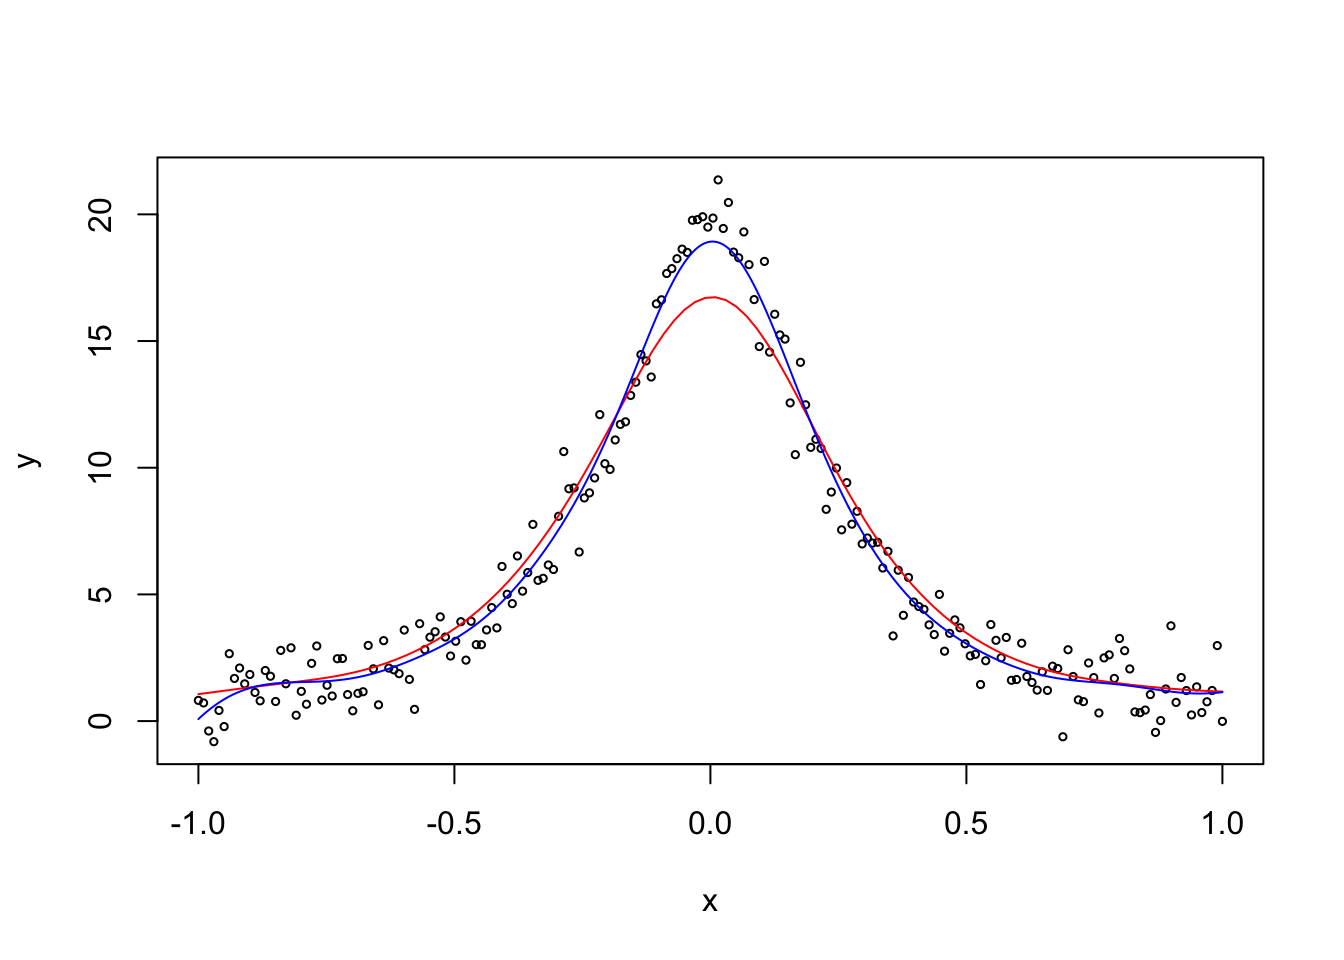
\includegraphics{MATH5714M_files/figure-latex/locpoly2-1.pdf}

We can see that the Nadaraya-Watson estimator (red line) is biased near the
peak, because all nearby samples correspond to smaller values of the mean line.
In contrast, the local polynomial estimate (blue line) has much lower bias.
\end{example}

\textbf{Summary}

\begin{itemize}
\tightlist
\item
  Regression with weights can be used to fit models to the data near
  a given point.
\item
  A simple application of linear regression can fit polynomials as well
  as straight lines.
\item
  The local polynomial regression estimator is a generalization of the
  Nadaraya-Watson estimator.
\end{itemize}

\clearpage

\hypertarget{X07-nearest}{%
\section{\texorpdfstring{\emph{k}-Nearest Neighbour Regression}{k-Nearest Neighbour Regression}}\label{X07-nearest}}

In the previous sections we used a fixed bandwidth \(h\) to determine the
scale on which ``closeness'' of existing samples to a new input \(x\) was
measured. While this approach generally works well, problems can appear
in regions where samples are sparse (\emph{e.g.}~in
example~\ref{exm:faithless}). This problem can be addressed by choosing
\(h\) adaptively, using larger bandwidths where samples are sparse and
smaller bandwidths in regions where there are many samples. The
\(k\)-nearest neighbour method is one of several methods which implements
this idea.

\hypertarget{definition-of-the-estimator}{%
\subsection{Definition of the Estimator}\label{definition-of-the-estimator}}

\begin{definition}
For \(k \in \{1, \ldots, n\}\), the \textbf{\emph{k}-nearest neighbour}, or
\(k\)-NN estimate for the model mean \(m(x)\) is given by
\begin{equation}
  \hat m_k(x)
  := \frac1k \sum_{i\in J_k(x)} y_i,  \label{eq:kNN}
\end{equation}
where
\begin{equation*}
  J_k(x)
  := \bigl\{ i \bigm| \mbox{$x_i$ is one of the $k$ nearest observations to $x$} \bigr\}.
\end{equation*}
\end{definition}

The \(k\)-NN estimate \(\hat m_k(x)\) is the average of the \(k\) responses
where the inputs are closest to~\(x\). We can interpret
equation~\eqref{eq:kNN} as a weighted average \begin{equation*}
  \hat m_k(x)
  = \sum_{i=1}^n w_i(x) y_i,
\end{equation*} where the weights are given by \begin{equation*}
  w_i(x)
  = \begin{cases}
      \frac1k, & \mbox{if $i \in J_k(x)$, and} \\
      0 & \mbox{otherwise.}
  \end{cases}
\end{equation*}

If several \(x_i\) have the same distance to \(x\), some tie-breaking rule
must be used to decide which indices to include in the set \(J_k(x)\).
This case is so unlikely that the choice of rule is not important. One
could, for example, pick one of the tied neighbours at random.

The method can be used both for the one-dimensional case \(x\in\mathbb{R}\), and
for vector-valued inputs \(x\in\mathbb{R}^p\). For the one-dimensional case, it is
advantageous to sort the data in order of increasing \(x_i\). In this
case, the position of \(x\) in the list of the \(x_i\) can be found using a
binary search, and the nearest neighbours can be identified by search to
the left and right of this position. For \(p > 1\) the method becomes
computationally very expensive, since the data needs to be sorted afresh
for every new input \(x\). Advanced data structures like \href{https://en.wikipedia.org/wiki/Cover_tree}{``cover trees''} can
be used to speed up the process of finding the nearest neighbours.

\hypertarget{properties}{%
\subsection{Properties}\label{properties}}

The parameter \(k\) controls the ``smoothness'' of the estimate. In the
extreme case \(k = n\), we have \(J_n(x) = \{1, \ldots, n\}\) and
\begin{equation*}
  \hat m_k(x)
  = \frac1n \sum_{i=1}^n y_i
\end{equation*} for all \(x\), \emph{i.e.}~for this case \(\hat m_k\) is
constant. The other extreme is the case of \(k=1\), where \(\hat m_k(x)\)
always equals the value of the closest \(x_i\) and has jumps at the
mid-points between the data points.

In the next section we will learn how \(k\) can be chosen using
cross-validation.

Independent of the value of \(k\), the function \(\hat m_k\) is always a
step function, with jumps at points \(x\) where two points have equal
distance from~\(x\).

\hypertarget{numerical-experiment}{%
\subsection{Numerical Experiment}\label{numerical-experiment}}

In R, an implementation of the \(k\)-NN method can be found in the \texttt{FNN} package.
This package implements not only \(k\)-NN regression, but also \(k\)-NN
classification, and it implements sophisticated algorithms to speed up the
search for the nearest neighbours in higher-dimensional spaces. The function
to perform \(k\)-NN regression is
\href{https://rdrr.io/cran/FNN/man/knn.reg.html}{\texttt{knn.reg()}}.

\begin{example}
Here we compute a \(k\)-NN estimate for the mean of the \texttt{faithful} dataset,
which we have already encountered in examples \ref{exm:faithful} and~\ref{exm:faithless}.
We start by storing the data in the variables \texttt{x} and \texttt{y}:

\begin{Shaded}
\begin{Highlighting}[]
\NormalTok{x }\OtherTok{\textless{}{-}}\NormalTok{ faithful}\SpecialCharTok{$}\NormalTok{eruptions}
\NormalTok{y }\OtherTok{\textless{}{-}}\NormalTok{ faithful}\SpecialCharTok{$}\NormalTok{waiting}
\end{Highlighting}
\end{Shaded}

Now we use \texttt{knn.reg()} to compute the \(k\)-NN estimate on a grid
of values. The help page for \texttt{knn.reg()} explains that we need to
convert the input to either a matrix or a data frame; here we use
data frames. The grid of input values where we want to estimate
the \(k\)-NN estimate is passed in via the optional argument \texttt{test\ =\ ...}.
Here we use the arbitrarily chosen value \(k = 50\).

\begin{Shaded}
\begin{Highlighting}[]
\FunctionTok{library}\NormalTok{(FNN)}

\NormalTok{x.test }\OtherTok{\textless{}{-}} \FunctionTok{seq}\NormalTok{(}\FloatTok{1.5}\NormalTok{, }\DecValTok{5}\NormalTok{, }\AttributeTok{length.out =} \DecValTok{500}\NormalTok{)}

\NormalTok{m }\OtherTok{\textless{}{-}} \FunctionTok{knn.reg}\NormalTok{(}\FunctionTok{data.frame}\NormalTok{(}\AttributeTok{x=}\NormalTok{x),}
             \AttributeTok{y =}\NormalTok{ y,}
             \AttributeTok{test =} \FunctionTok{data.frame}\NormalTok{(}\AttributeTok{x=}\NormalTok{x.test),}
             \AttributeTok{k =} \DecValTok{50}\NormalTok{)}

\FunctionTok{plot}\NormalTok{(x, y, }\AttributeTok{cex=}\NormalTok{.}\DecValTok{5}\NormalTok{)}
\FunctionTok{lines}\NormalTok{(x.test, m}\SpecialCharTok{$}\NormalTok{pred, }\AttributeTok{col =} \StringTok{"blue"}\NormalTok{)}
\end{Highlighting}
\end{Shaded}

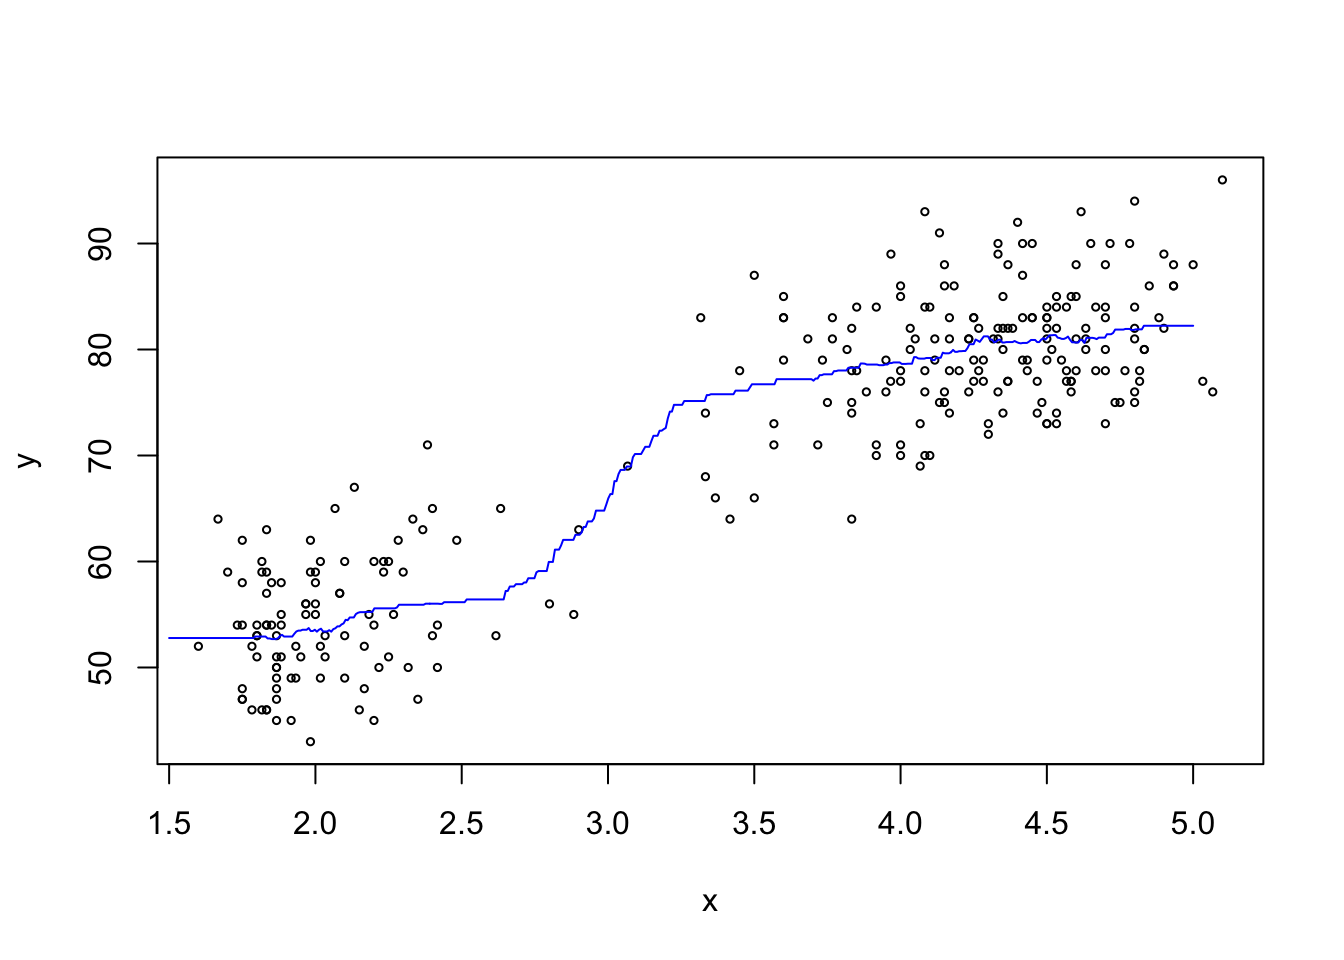
\includegraphics{MATH5714M_files/figure-latex/faithful-kNN-1.pdf}

The estimated mean curve looks reasonable.
\end{example}

\hypertarget{variants-of-the-method}{%
\subsection{Variants of the Method}\label{variants-of-the-method}}

\begin{itemize}
\item
  For one-dimensional inputs and even \(k\), the \textbf{symmetric \emph{k}-NN
  estimate} averages the responses corresponding to the \(k/2\) nearest
  neighbours smaller than \(x\) and the \(k/2\) nearest neighbours larger
  than~\(x\).
\item
  To obtain a continuous estimate, we can define a ``local bandwidth''
  \(h(x)\) as \begin{equation*}
    h(x) = c \max\bigl\{ |x - x_i| \bigm| i \in J_k(x) \bigr\}
  \end{equation*} for some constant~\(c\), and then use the
  Nadaraya-Watson estimator with this bandwidth: \begin{equation*}
    \tilde m(x)
    = \frac{\sum_{i=1}^n K_{h(x)}(x - x_i) y_i}{\sum_{j=1}^n K_{h(x)}(x - x_j)},
  \end{equation*} where \(K\) is a kernel function as before. If we use
  \(c = 1\) together with the uniform kernel \begin{equation*}
    K(x)
    = \begin{cases}
        1/2 & \mbox{if $-1 \leq x \leq 1$} \\
        0 & \mbox{otherwise,}
      \end{cases}
  \end{equation*} this method coincides with the \(k\)-NN estimator.
\end{itemize}

\clearpage

\hypertarget{X08-xval}{%
\section{Cross-validation}\label{X08-xval}}

In this section we will discuss methods for chosing the bandwidth~\(h\)
for kernel-based methods, and the size \(k\) of the neighbourhood used
in \(k\)-nearest neighbour regression. The methods we will use here
are based on cross-validation.

The idea of cross-validation is to measure goodness of fit by comparing each
sample \(y_i\) to a fitted value \(\tilde y_i\), where the fitted values \(\tilde y_i\) are computed from a subset of the data which excludes \(x_i\). There are
different ways to implement this idea:

\begin{itemize}
\item
  In \textbf{leave-one-out cross-validation}, a separate model is fitted
  for each \(i \in \{1, \ldots, n\}\), leaving out just the sample \((x_i, y_i)\)
  for this model. This method can be computationally
  expensive for large \(n\), since \(n\) models need to be fitted to the data.
\item
  In \textbf{\emph{k}-fold cross-validation}, the data is partitioned into
  \(k\) subsamples of approximately equal size. Only \(k\) models are fitted,
  each one leaving out the data from one subsample. Then for every \(i\)
  there is exactly one model which does not use \((x_i, y_i)\), and
  to compute the fitted value for \((x_i, y_i)\), we use this model.
  Since fewer data are used to fit each model, this method gives less
  accurate results than leave-one-out cross-validation.
  For this method to work, it is important that the subsamples
  are independent of each other.
\end{itemize}

The idea behind cross-validation is that we always compare \(y_i\) to
a fitted value which was computed without using any information about
the true value of \(y_i\). This way, a method cannot achive a misleadingly
good fit by overfitting the data.

\hypertarget{regression}{%
\subsection{Regression}\label{regression}}

In linear regression, we find the regression line by minimising
the residual sum of squares. One could be tempted to try the same
approach here and to find the ``best'' \(h\) by minimising
\begin{equation*}
  r(h)
  := \sum_{i=1}^n \bigl( y_i - \hat m_h(x_i) \bigr)^2.
\end{equation*}
Unfortunately, this approach does not work: for \(h \downarrow 0\)
we have \(\hat m_h(x_i) \to y_i\) and thus \(r(h) \to 0\). For this reason,
minimising \(r(h)\) always finds \(h=0\) as the optimal value of~\(h\).
To solve the problem we use leave-one-out cross validation and minimise
\begin{equation*}
  r_\mathrm{LOO}(h)
  := \sum_{i=1}^n \bigl( y_i - \hat m^{(i)}_h(x_i) \bigr)^2
\end{equation*}
instead,
where \(m^{(i)}\) is the kernel regression estimate computed without using
sample~\(i\):
\begin{equation*}
  \hat m_h^{(i)}(x)
  = \frac{\sum_{j \;\mid\; j\neq i} K_h(x - x_j)y_j}{\sum_{j \;\mid\; j\neq i}K_h(x - x_j)}
\end{equation*}
for the Nadaraya-Watson Estimator and similarly for local polynomial
regression.

A similar approach can be used to find the optimal \(k\) for
a \(k\)-nearest neighbour estimate.

\hypertarget{kernel-density-estimation-1}{%
\subsection{Kernel Density Estimation}\label{kernel-density-estimation-1}}

When using kernel density estimation in practice, we need to choose the
bandwidth~\(h\). One idea for finding a good \(h\) is by using
maximum likelihood estimation: We could try to
choose \(h\) to maximize the likelihood
\begin{equation*}
  L(h;x_1, \ldots, x_n)
  = \prod_{i=1}^n \hat f_h(x_i),
\end{equation*}
but this gives the solution \(h=0\). So, instead we maximize the
leave-one-out estimate of the log likelihood, which is given by
\begin{equation*}
  L_\mathrm{LOO}(h;x_1, \ldots, x_n)
  = \prod_{i=1}^n \hat f^{(i)}_h(x_i).
\end{equation*}
This technique is known as \textbf{maximum likelihood cross-validation}.
When this method is used in practice, it is advantageous to minimise
\begin{align*}
  \mathcal{L}_\mathrm{LOO}(h;x_1, \ldots, x_n)
  &:= \log\Bigl( L_\mathrm{LOO}(h;x_1, \ldots, x_n) \Bigr) \\
  &= \log\Bigl( \prod_{i=1}^n \hat f^{(i)}_h(x_i) \Bigr) \\
  &= \sum_{i=1}^n \log\bigl( \hat f^{(i)}_h(x_i) \bigr)
\end{align*}
instead of \(L_\mathrm{LOO}\), since the product in the definition
of the likelihood can be strongly affected by numerical errors.

An alternative method to find a good \(h\) considers the
integrated mean squared error (IMSE) as a measure for the error.
This is the same quantity we also used to derive our theoretical results:
\begin{equation*}
  \mathrm{IMSE}\bigl( \hat f_h \bigr)
  = \int_{-\infty}^\infty \mathop{\mathrm{MSE}}\nolimits\bigl( \hat f_h(x) \bigr) \,dx.
\end{equation*}
Unfortunately, the \(h\) which minimises this expression depends
on properties of \(h\) and in section~\ref{bwsel} we were only
able to find a heuristic ``plug-in'' estimate to approximate the best~\(h\).
The following lemma shows how a variant of leave-one-out cross-validation
can be used to estimate the optimal~\(h\) from data.

\begin{lemma}
\protect\hypertarget{lem:KDE-XV}{}\label{lem:KDE-XV}

Let \(\hat h_h\) be the kernel density estimate with bandwidth~\(h\)
and let
\begin{equation*}
  e(h)
  := \int \mathbb{E}\bigl( \hat f_h(x)^2 \bigr) dx - 2 \int \mathbb{E}\bigl( \hat f_h(x) \bigr) f(x) dx.
\end{equation*}
Then the following statements hold.

\begin{enumerate}
\def\labelenumi{(\alph{enumi})}
\item
  We have
  \(\mathrm{IMSE}\bigl( \hat f_h \bigr) = e(h) + \mathrm{const}\),
  where \(\mathrm{const}\) stands for a term which does not depend on \(h\).
\item
  Let \(f_h^{(i)}\) be the kernel density estimate computed from the data
  with sample \(i\) omitted.
  Then
  \begin{equation*}
    \mathrm{CV}(h)
    := \int \hat f_h(x)^2 dx - \frac{2}{n}\sum_{i=1}^n \hat f_h^{(i)}(x_i)
  \end{equation*}
  is an (approximately) unbiased estimator for~\(e(h)\).
\end{enumerate}

\end{lemma}

\begin{proof}
For the first statement can be shown by expanding the square in the
definition of the (I)MSE:
\begin{align*}
  \mathrm{IMSE}\bigl( \hat f_h \bigr)
  &= \int_{-\infty}^\infty \mathop{\mathrm{MSE}}\nolimits\bigl( \hat f_h(x) \bigr) \,dx \\
  &= \int_{-\infty}^\infty \mathbb{E}\Bigl( \bigl( \hat f_h(x) - f(x) \bigr)^2 \Bigr) \,dx \\
  &= \int_{-\infty}^\infty \mathbb{E}\Bigl( \hat f_h(x)^2 - 2 \hat f(x) f(x)  + f(x)^2 \Bigr) \,dx \\
  &= \int_{-\infty}^\infty \mathbb{E}\Bigl( \hat f_h(x)^2 \Bigr) \,dx
         - 2 \int_{-\infty}^\infty \mathbb{E}\Bigl( \hat f(x) f(x) \Bigr) \,dx \\
      &\hskip5cm
         + \int_{-\infty}^\infty \mathbb{E}\Bigl( f(x)^2 \Bigr) \,dx \\
  &= \int_{-\infty}^\infty \mathbb{E}\Bigl( \hat f_h(x)^2 \Bigr) \,dx
         - 2 \int_{-\infty}^\infty \mathbb{E}\bigl( \hat f(x) \bigr) f(x) \,dx \\
      &\hskip5cm
         + \int_{-\infty}^\infty f(x)^2 \,dx,
\end{align*}
where we used the fact that \(f(x)\) is not random.
Since the last term does not depend on \(h\), the first claim is proved.

For the second statement we need to consider the kernel density estimates
computed from random data \(X_1, \ldots, X_n \sim f\), i.i.d. We have to show
that
\begin{equation*}
  \mathbb{E}\bigl( \mathrm{CV}(h) \bigr)
  = e(h)
  = \int \mathbb{E}\bigl( \hat f_h(x)^2 \bigr) dx - 2 \int \mathbb{E}\bigl( \hat f_h(x) \bigr) f(x) dx.
\end{equation*}
For the first term in the definition of \(\mathrm{CV}\) we get
\begin{equation*}
  \mathbb{E}\Bigl( \int \hat f_h(x)^2 dx \Bigr)
  = \int \mathbb{E}\bigl( \hat f_h(x)^2 \bigr) dx,
\end{equation*}
where we used Fubini's theorem to exchange the expectation with the integral.
For the second term we have
\begin{align*}
  \mathbb{E}\Bigl( \frac{1}{n} \sum_{i=1}^n \hat f_h^{(i)}(X_i) \Bigr)
  &= \frac{1}{n} \sum_{i=1}^n \mathbb{E}\Bigl( \hat f_h^{(i)}(X_i) \Bigr) \\
  &= \mathbb{E}\Bigl( \hat f_h^{(1)}(X_1) \Bigr),
\end{align*}
since the \(X_i\) are independent and identically distributed.
Since the estimator \(f_h^{(1)}\) is computed from \(X_2, \ldots, X_n\),
which are independent of \(X_1\), we can evaluate the expecation on
the right-hand side by first computing \(\mathbb{E}\Bigl( \hat f_h^{(1)}(x) \Bigr)\)
as a function of \(x\), then using \(X_1\) in place of \(x\), and computing
the expecation over \(X_1\) afterwards. This gives
\begin{align*}
  \mathbb{E}\Bigl( \frac{1}{n} \sum_{i=1}^n \hat f_h^{(i)}(X_i) \Bigr)
  &= \mathbb{E}\Bigl( \mathbb{E}\bigl( \hat f_h^{(1)}(X_1) \bigm| X_1 \bigr) \Bigr) \\
  &= \int \mathbb{E}\bigl( \hat f_h^{(1)}(x) \bigr) \, f(x) \, dx,
\end{align*}
since \(X_1 \sim f\). Finally, since \(\hat f_h^{(1)}\) and \(\hat f_h\)
only differ in the sample size, by using \(n-1\) and \(n\) samples respectively,
we have
\begin{equation*}
  \mathbb{E}\bigl( \hat f_h^{(1)}(x) \bigr)
  \approx \mathbb{E}\bigl( \hat f_h(x) \bigr).
\end{equation*}
Combining these equations completes the proof.
\end{proof}

Using the result from the lemma we see that we can choose \(h\)
to minimise \(\mathrm{CV}(h)\) in order to get a candidate for the
bandwidth \(h\). This procedure is known as
\textbf{integrated squared error cross-validation}.

These two approaches differ slightly in the optimal \(h\), but the first one is
easier to implement as there is no integration involved.

\textbf{Summary}

\begin{itemize}
\tightlist
\item
  Cross-validation can be used to avoid overfitting the data when we choose~\(h\).
\item
  We have seen how to estimate \(h\) for kernel-based methods,
  and \(k\) for \(k\)-NN regression estimates.
\end{itemize}

\clearpage

\hypertarget{X09-examples}{%
\section{Examples}\label{X09-examples}}

To conclude these notes, we give three examples where we use
cross-validation to choose the tuning parameter in kernel
density estimation, kernel regression, and k-nearest neighbour
regression.

\hypertarget{kernel-density-estimation-2}{%
\subsection{Kernel Density Estimation}\label{kernel-density-estimation-2}}

Here we show how to find a good bandwidth for Kernel Density Estimation,
by using cross-validation. From lemma~\ref{lem:KDE-XV} we know that
we can choose the \(h\) which minimises
\begin{equation}
  \mathrm{CV}(h)
  = \int \hat f_h(x)^2 dx - \frac{2}{n}\sum_{i=1}^n \hat f_h^{(i)}(x_i)
  =: A - B.  \label{eq:CVh}
\end{equation}

We will consider the
\href{https://teaching.seehuhn.de/data/buffalo/}{snow fall dataset}
again:

\begin{Shaded}
\begin{Highlighting}[]
\CommentTok{\# data from https://teaching.seehuhn.de/data/buffalo/}
\NormalTok{buffalo }\OtherTok{\textless{}{-}} \FunctionTok{read.csv}\NormalTok{(}\StringTok{"data/buffalo.csv"}\NormalTok{)}
\NormalTok{x }\OtherTok{\textless{}{-}}\NormalTok{ buffalo}\SpecialCharTok{$}\NormalTok{snowfall}
\NormalTok{n }\OtherTok{\textless{}{-}} \FunctionTok{length}\NormalTok{(x)}
\end{Highlighting}
\end{Shaded}

In order to speed up the computation of the \(f_h^{(i)}\), we implement
the kernel density estimate ``by hand''. Thus, instead of using the built-in
function \texttt{density}, we use the formula
\begin{equation*}
  \hat f_h(x)
  = \frac{1}{n} \sum_{i=1}^n K_h(x - x_i).
\end{equation*}
from definition~\ref{def:KDE}.

We use a number of ``tricks'' in the R code:

\begin{itemize}
\tightlist
\item
  For numerically computing the integral of \(\hat f_h^2\) in term~\(A\)
  we evaluate \(\hat f_h\) on a grid of \(x\)-values,
  say \(\tilde x_1, \ldots, \tilde x_m\).
\item
  When computing \(\hat f_h(\tilde x_j)\)
  we need to compute all pair differences \(\tilde x_j - x_i\). In R, this can
  efficiently be done using the command \texttt{outer(x,\ x.tilde,\ "-")},
  which returns the pair differences as an \(n \times m\) matrix.
\item
  Here we use a Gaussian kernel, so that \(K_h\) can be evaluated using
  \texttt{dnorm(...,\ sd\ =\ h)} in R. This function can be applied to the
  matrix of pair differences; the result is a matrix \texttt{K} where row~\(i\),
  column~\(j\) stores the value \(K_h(\tilde x_j - x_i)\).
\item
  The kernel density estimate \(\hat f_h\) now corresponds to the
  column means of the matrix \texttt{K}. In R, these can be efficiently computed
  using the command \texttt{colMeans()}.
\item
  Term \(A\) in equation~\eqref{eq:CVh} can now be approximate by
  the sum of the \(\hat f_h(\tilde x_j)\), multiplied by the distance
  between the grid points:
  \begin{equation*}
    A
    = \int \hat f_h(x)^2 \,dx
    \approx \sum_{j=1}^m \hat f_h(\tilde x_j)^2  \, \Delta \tilde x.
  \end{equation*}
\item
  To compute term \(B\) in equation~\eqref{eq:CVh}, we can use
  the formula
  \begin{align*}
    \sum_{j=1}^n \hat f_h^{(j)}(x_j)
    &= \sum_{j=1}^n \frac{1}{n-1} \sum_{i\neq j} K_h(x_j - x_i) \\
    &= \frac{1}{n-1} \sum_{i,j=1 \atop i\neq j}^n K_h(x_j - x_i).
  \end{align*}
  Here we can use \texttt{outer()} again, and then implement the condition
  \(i\neq j\) by setting the matrix elements corresponding to \(i=j\)
  equal to 0 before taking the sum.
\end{itemize}

Using these ideas, we can implement the function \(\mathrm{cv}(h)\)
in R as follows:

\begin{Shaded}
\begin{Highlighting}[]
\NormalTok{cv.h }\OtherTok{\textless{}{-}} \ControlFlowTok{function}\NormalTok{(h) \{}
\NormalTok{    x.min }\OtherTok{\textless{}{-}} \FunctionTok{min}\NormalTok{(x) }\SpecialCharTok{{-}} \DecValTok{3}\SpecialCharTok{*}\NormalTok{h}
\NormalTok{    x.max }\OtherTok{\textless{}{-}} \FunctionTok{max}\NormalTok{(x) }\SpecialCharTok{+} \DecValTok{3}\SpecialCharTok{*}\NormalTok{h}
\NormalTok{    m }\OtherTok{\textless{}{-}} \DecValTok{1000}
\NormalTok{    dx }\OtherTok{\textless{}{-}}\NormalTok{ (x.max }\SpecialCharTok{{-}}\NormalTok{ x.min) }\SpecialCharTok{/}\NormalTok{ (m }\SpecialCharTok{{-}} \DecValTok{1}\NormalTok{)}
\NormalTok{    x.tilde }\OtherTok{\textless{}{-}} \FunctionTok{seq}\NormalTok{(x.min, x.max, }\AttributeTok{length.out =}\NormalTok{ m)}

\NormalTok{    K }\OtherTok{\textless{}{-}} \FunctionTok{dnorm}\NormalTok{(}\FunctionTok{outer}\NormalTok{(x, x.tilde, }\StringTok{"{-}"}\NormalTok{), }\AttributeTok{sd =}\NormalTok{ h)}
\NormalTok{    f.hat }\OtherTok{\textless{}{-}} \FunctionTok{colMeans}\NormalTok{(K)}
\NormalTok{    A }\OtherTok{\textless{}{-}} \FunctionTok{sum}\NormalTok{(f.hat}\SpecialCharTok{\^{}}\DecValTok{2} \SpecialCharTok{*}\NormalTok{ dx)}

\NormalTok{    K }\OtherTok{\textless{}{-}} \FunctionTok{dnorm}\NormalTok{(}\FunctionTok{outer}\NormalTok{(x, x, }\StringTok{"{-}"}\NormalTok{), }\AttributeTok{sd =}\NormalTok{ h)}
    \FunctionTok{diag}\NormalTok{(K) }\OtherTok{\textless{}{-}} \DecValTok{0}
\NormalTok{    B }\OtherTok{\textless{}{-}} \DecValTok{2} \SpecialCharTok{*} \FunctionTok{sum}\NormalTok{(K) }\SpecialCharTok{/}\NormalTok{ (n}\DecValTok{{-}1}\NormalTok{) }\SpecialCharTok{/}\NormalTok{ n}

    \FunctionTok{return}\NormalTok{(A }\SpecialCharTok{{-}}\NormalTok{ B)}
\NormalTok{\}}
\end{Highlighting}
\end{Shaded}

Finally, we evaluate the function \texttt{cv.h()} on a grid of \(h\)-values
to find a good value of~\(h\):

\begin{Shaded}
\begin{Highlighting}[]
\NormalTok{h }\OtherTok{\textless{}{-}} \DecValTok{10}\SpecialCharTok{\^{}}\FunctionTok{seq}\NormalTok{(}\SpecialCharTok{{-}}\DecValTok{1}\NormalTok{, }\DecValTok{3}\NormalTok{, }\AttributeTok{length.out =} \DecValTok{41}\NormalTok{)}
\NormalTok{cv }\OtherTok{\textless{}{-}} \FunctionTok{numeric}\NormalTok{(}\FunctionTok{length}\NormalTok{(h))}
\ControlFlowTok{for}\NormalTok{ (i }\ControlFlowTok{in} \FunctionTok{seq\_along}\NormalTok{(h)) \{}
\NormalTok{    cv[i] }\OtherTok{\textless{}{-}} \FunctionTok{cv.h}\NormalTok{(h[i])}
\NormalTok{\}}
\FunctionTok{plot}\NormalTok{(h, cv, }\AttributeTok{log=}\StringTok{"x"}\NormalTok{, }\AttributeTok{type =} \StringTok{"l"}\NormalTok{)}

\NormalTok{best.h }\OtherTok{\textless{}{-}}\NormalTok{ h[}\FunctionTok{which.min}\NormalTok{(cv)]}
\FunctionTok{abline}\NormalTok{(}\AttributeTok{v =}\NormalTok{ best.h)}
\end{Highlighting}
\end{Shaded}

\includegraphics{MATH5714M_files/figure-latex/cv-KDE-1.pdf}

The optimal bandwidth is \(h = 12.59\).
The kernel density estimate using this \(h\) is shown in the following figure.

\begin{Shaded}
\begin{Highlighting}[]
\NormalTok{x.min }\OtherTok{\textless{}{-}} \FunctionTok{min}\NormalTok{(x) }\SpecialCharTok{{-}} \DecValTok{3}\SpecialCharTok{*}\NormalTok{best.h}
\NormalTok{x.max }\OtherTok{\textless{}{-}} \FunctionTok{max}\NormalTok{(x) }\SpecialCharTok{+} \DecValTok{3}\SpecialCharTok{*}\NormalTok{best.h}
\NormalTok{m }\OtherTok{\textless{}{-}} \DecValTok{100}
\NormalTok{x.tilde }\OtherTok{\textless{}{-}} \FunctionTok{seq}\NormalTok{(x.min, x.max, }\AttributeTok{length.out =}\NormalTok{ m)}

\NormalTok{K }\OtherTok{\textless{}{-}} \FunctionTok{dnorm}\NormalTok{(}\FunctionTok{outer}\NormalTok{(x, x.tilde, }\StringTok{"{-}"}\NormalTok{), }\AttributeTok{sd =}\NormalTok{ best.h)}
\NormalTok{f.hat }\OtherTok{\textless{}{-}} \FunctionTok{colMeans}\NormalTok{(K)}

\FunctionTok{plot}\NormalTok{(x.tilde, f.hat, }\AttributeTok{type =} \StringTok{"l"}\NormalTok{,}
     \AttributeTok{xlab =} \StringTok{"snowfall [in]"}\NormalTok{, }\AttributeTok{ylab =} \StringTok{"density"}\NormalTok{)}
\end{Highlighting}
\end{Shaded}

\includegraphics{MATH5714M_files/figure-latex/cv-KDE-best-1.pdf}

\hypertarget{kernel-regression}{%
\subsection{Kernel Regression}\label{kernel-regression}}

To illustrate cross-validation for the different smoothing methods,
we use the \texttt{faithful} dataset again.

\begin{Shaded}
\begin{Highlighting}[]
\NormalTok{x }\OtherTok{\textless{}{-}}\NormalTok{ faithful}\SpecialCharTok{$}\NormalTok{eruptions}
\NormalTok{y }\OtherTok{\textless{}{-}}\NormalTok{ faithful}\SpecialCharTok{$}\NormalTok{waiting}
\end{Highlighting}
\end{Shaded}

We compare the methods using the leave-one-out mean squared error
\begin{equation*}
  r(h)
  = \frac1n \sum_{i=1}^n \bigl( y_i - \hat m^{(i)}(x_i) \bigr)^2.
\end{equation*}

We start by considering the Nadaraya-Watson estimator.
Here we have to compute
\begin{equation*}
  \hat m^{(i)}_h(x_i)
  = \frac{\sum_{j=1, j\neq i}^n K_h(x_i - x_j) y_j}{\sum_{j=1, j\neq i}^n K_h(x_i - x_j)}
\end{equation*}
for all \(i\in\{1, \ldots, n\}\).
To evaluate this expression in R, we use the same ideas as before:

\begin{itemize}
\tightlist
\item
  We use \texttt{outer(x,\ x,\ "-")} to compute all pair differences \(x_i - x_j\).
\item
  We use \texttt{dnorm(...,\ sd\ =\ h)} to compute \(K_h\).
\item
  We can obtain the leave-one-out estimate by setting the diagonal
  of \(K\) to zero.
\end{itemize}

One new idea is needed to compute the products \(K_h(x_i - x_j) y_j\)
in an efficient way:

\begin{itemize}
\tightlist
\item
  If we ``multiply'' a matrix \texttt{K} to a vector \texttt{y} using \texttt{*} (instead of using
  \texttt{\%*\%} for the usual matrix vector multiplication), the product is
  performed element-wise. If \texttt{y} has as many elements as \texttt{K} has rows,
  then the results is the matrix \((k_{ij}y_i)_{i,j}\), \emph{i.e.} each row
  of \texttt{K} is multiplied with the corresponding element of~\texttt{y}.
\end{itemize}

Combining these ideas, we get the following function
to compute the leave-one-out estimate for the mean squared error of
the Nadaraya-Watson estimator:

\begin{Shaded}
\begin{Highlighting}[]
\NormalTok{r.NW }\OtherTok{\textless{}{-}} \ControlFlowTok{function}\NormalTok{(h) \{}
\NormalTok{    K }\OtherTok{\textless{}{-}} \FunctionTok{dnorm}\NormalTok{(}\FunctionTok{outer}\NormalTok{(x, x, }\StringTok{"{-}"}\NormalTok{), }\AttributeTok{sd =}\NormalTok{ h)}

    \CommentTok{\# compute a leave{-}one{-}out estimate}
    \FunctionTok{diag}\NormalTok{(K) }\OtherTok{\textless{}{-}} \DecValTok{0}

\NormalTok{    m.hat }\OtherTok{\textless{}{-}} \FunctionTok{colSums}\NormalTok{(K}\SpecialCharTok{*}\NormalTok{y) }\SpecialCharTok{/} \FunctionTok{colSums}\NormalTok{(K)}
    \FunctionTok{mean}\NormalTok{((m.hat }\SpecialCharTok{{-}}\NormalTok{ y)}\SpecialCharTok{\^{}}\DecValTok{2}\NormalTok{)}
\NormalTok{\}}
\end{Highlighting}
\end{Shaded}

We will also consider local linear smoothing, \emph{i.e.} local polynomial
smoothing where the degree \(p\) of the polynomials is \(p=1\).
As we have seen in the section about \protect\hyperlink{polynomial-regression-with-weights}{Polynomial Regression with Weights},
the local linear estimator can be computed as
\begin{equation*}
  \hat m_h(x)
  = e_0^\top (X^\top W X)^{-1} X^\top W y,
\end{equation*}
where \(X\) and \(W\) are defined as in equations \eqref{eq:X-local}
and~\eqref{eq:W-diagonal}.
Here we use the ``linear'' case (\(p=1\)) instead of the polynomial case (\(p\geq 1\)).
For this case it is easy to check that we have
\begin{equation*}
  X^\top W X
  = \begin{pmatrix}
        \sum_j K_h(x-x_j)     & \sum_j K_h(x-x_j) x_j   \\
        \sum_j K_h(x-x_j) x_j & \sum_j K_h(x-x_j) x_j^2
    \end{pmatrix}
\end{equation*}
and
\begin{equation*}
  X^\top W y
  = \begin{pmatrix}
        \sum_j K_h(x-x_j) y_j     \\
        \sum_j K_h(x-x_j) x_j y_j
    \end{pmatrix}.
\end{equation*}
Using the formula
\begin{equation*}
  \begin{pmatrix}
    a & b \\
    c & d
  \end{pmatrix}^{-1}
  = \frac{1}{ad-bc} \begin{pmatrix}
    d & -b \\
    -c & a
  \end{pmatrix}
\end{equation*}
for the inverse of a general \(2\times 2\)-matrix, we find
\begin{equation*}
  \hat m_h(x)
  = \frac{T_1 T_2 - T_3 T_4}{B_1 B_2 - B_3^2},
\end{equation*}
where
\begin{align*}
  T_1 &= \sum_{j=1}^n K_h(x-x_j) y_j       , \\
  T_2 &= \sum_{j=1}^n K_h(x-x_j) x_j(x_j-x), \\
  T_3 &= \sum_{j=1}^n K_h(x-x_j) x_j y_j   , \\
  T_4 &= \sum_{j=1}^n K_h(x-x_j) (x_j-x)   , \\
  B_1 &= \sum_{j=1}^n K_h(x-x_j)           , \\
  B_2 &= \sum_{j=1}^n K_h(x-x_j) x_j^2     , \\
  B_3 &= \sum_{j=1}^n K_h(x-x_j) x_j       .
\end{align*}
As before, for a leave-one-out estimate we need to compute these sums over all
\(j\neq i\). Since each of the seven terms listed above contains the term
\(K_h(x-x_j)\) inside the sum, we can achieve this by setting the corresponing
elements of the matrix \texttt{K} to zero.

\begin{Shaded}
\begin{Highlighting}[]
\NormalTok{r.LL }\OtherTok{\textless{}{-}} \ControlFlowTok{function}\NormalTok{(h) \{}
\NormalTok{    dx }\OtherTok{\textless{}{-}} \FunctionTok{outer}\NormalTok{(x, x, }\StringTok{"{-}"}\NormalTok{)}
\NormalTok{    K }\OtherTok{\textless{}{-}} \FunctionTok{dnorm}\NormalTok{(dx, }\AttributeTok{sd =}\NormalTok{ h)}

    \CommentTok{\# compute a leave{-}one{-}out estimate}
    \FunctionTok{diag}\NormalTok{(K) }\OtherTok{\textless{}{-}} \DecValTok{0}

\NormalTok{    T1 }\OtherTok{\textless{}{-}} \FunctionTok{colSums}\NormalTok{(y}\SpecialCharTok{*}\NormalTok{K)}
\NormalTok{    T2 }\OtherTok{\textless{}{-}} \FunctionTok{colSums}\NormalTok{(x}\SpecialCharTok{*}\NormalTok{dx}\SpecialCharTok{*}\NormalTok{K)}
\NormalTok{    T3 }\OtherTok{\textless{}{-}} \FunctionTok{colSums}\NormalTok{(x}\SpecialCharTok{*}\NormalTok{y}\SpecialCharTok{*}\NormalTok{K)}
\NormalTok{    T4 }\OtherTok{\textless{}{-}} \FunctionTok{colSums}\NormalTok{(dx}\SpecialCharTok{*}\NormalTok{K)}
\NormalTok{    B1 }\OtherTok{\textless{}{-}} \FunctionTok{colSums}\NormalTok{(K)}
\NormalTok{    B2 }\OtherTok{\textless{}{-}} \FunctionTok{colSums}\NormalTok{(x}\SpecialCharTok{\^{}}\DecValTok{2}\SpecialCharTok{*}\NormalTok{K)}
\NormalTok{    B3 }\OtherTok{\textless{}{-}} \FunctionTok{colSums}\NormalTok{(x}\SpecialCharTok{*}\NormalTok{K)}
\NormalTok{    m.hat }\OtherTok{\textless{}{-}}\NormalTok{ (T1}\SpecialCharTok{*}\NormalTok{T2 }\SpecialCharTok{{-}}\NormalTok{ T3}\SpecialCharTok{*}\NormalTok{T4) }\SpecialCharTok{/}\NormalTok{ (B1}\SpecialCharTok{*}\NormalTok{B2 }\SpecialCharTok{{-}}\NormalTok{ B3}\SpecialCharTok{\^{}}\DecValTok{2}\NormalTok{)}

    \FunctionTok{mean}\NormalTok{((m.hat }\SpecialCharTok{{-}}\NormalTok{ y)}\SpecialCharTok{\^{}}\DecValTok{2}\NormalTok{)}
\NormalTok{\}}
\end{Highlighting}
\end{Shaded}

Now we evaluate the function \texttt{r.NW()} and \texttt{r.LL()} on a grid of \(h\)-values
to find the optimal \(h\) for each method.

\begin{Shaded}
\begin{Highlighting}[]
\NormalTok{h }\OtherTok{\textless{}{-}} \DecValTok{10}\SpecialCharTok{\^{}}\FunctionTok{seq}\NormalTok{(}\SpecialCharTok{{-}}\FloatTok{1.4}\NormalTok{, }\FloatTok{0.1}\NormalTok{, }\AttributeTok{length.out =} \DecValTok{61}\NormalTok{)}
\NormalTok{mse.nw }\OtherTok{\textless{}{-}} \FunctionTok{numeric}\NormalTok{(}\FunctionTok{length}\NormalTok{(h))}
\NormalTok{mse.ll }\OtherTok{\textless{}{-}} \FunctionTok{numeric}\NormalTok{(}\FunctionTok{length}\NormalTok{(h))}
\ControlFlowTok{for}\NormalTok{ (i }\ControlFlowTok{in} \FunctionTok{seq\_along}\NormalTok{(h)) \{}
\NormalTok{    mse.nw[i] }\OtherTok{\textless{}{-}} \FunctionTok{r.NW}\NormalTok{(h[i])}
\NormalTok{    mse.ll[i] }\OtherTok{\textless{}{-}} \FunctionTok{r.LL}\NormalTok{(h[i])}
\NormalTok{\}}
\FunctionTok{plot}\NormalTok{(h, mse.nw, }\AttributeTok{log=}\StringTok{"x"}\NormalTok{, }\AttributeTok{type =} \StringTok{"l"}\NormalTok{, }\AttributeTok{ylim =} \FunctionTok{range}\NormalTok{(mse.nw, mse.ll),}
     \AttributeTok{ylab =} \StringTok{"leave{-}one{-}out MSE"}\NormalTok{)}
\FunctionTok{lines}\NormalTok{(h, mse.ll, }\AttributeTok{col=}\StringTok{"red"}\NormalTok{)}

\NormalTok{best.h.NW }\OtherTok{\textless{}{-}}\NormalTok{ h[}\FunctionTok{which.min}\NormalTok{(mse.nw)]}
\FunctionTok{abline}\NormalTok{(}\AttributeTok{v =}\NormalTok{ best.h.NW)}
\NormalTok{best.h.LL }\OtherTok{\textless{}{-}}\NormalTok{ h[}\FunctionTok{which.min}\NormalTok{(mse.ll)]}
\FunctionTok{abline}\NormalTok{(}\AttributeTok{v =}\NormalTok{ best.h.LL, }\AttributeTok{col=}\StringTok{"red"}\NormalTok{)}
\end{Highlighting}
\end{Shaded}

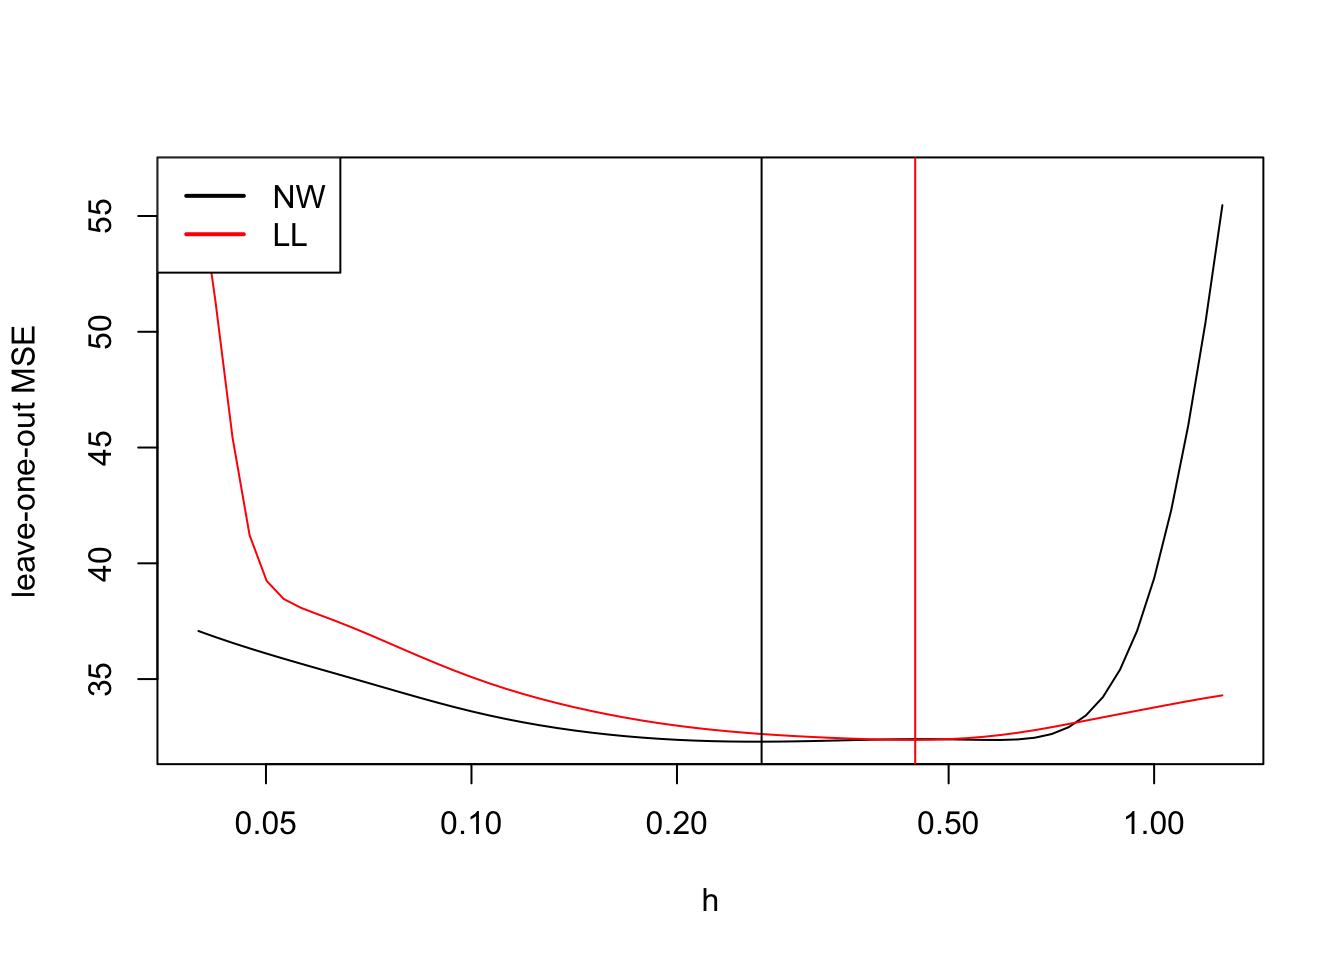
\includegraphics{MATH5714M_files/figure-latex/cv-loclin-1.pdf}

As expected, the optimal bandwidth for local linear regression is
larger than for the Nadaraya Watson estimator.

\hypertarget{k-nearest-neighbour-regression}{%
\subsection{\texorpdfstring{\emph{k}-Nearest Neighbour Regression}{k-Nearest Neighbour Regression}}\label{k-nearest-neighbour-regression}}

To conclude this section we use leave-one-out cross-validation to determine the
optimal \(k\) for \(k\)-nearest neighbour regression. Here it seems difficult to
make any savings, so we resort to simply fitting \(n\) different models in the
naive way. For this reason, the code in this section is much slower to
run than the code in the previous sections.

\begin{Shaded}
\begin{Highlighting}[]
\NormalTok{k }\OtherTok{\textless{}{-}} \DecValTok{10}\SpecialCharTok{:}\DecValTok{70}
\NormalTok{mse.knn }\OtherTok{\textless{}{-}} \FunctionTok{numeric}\NormalTok{(}\FunctionTok{length}\NormalTok{(k))}
\ControlFlowTok{for}\NormalTok{ (j }\ControlFlowTok{in} \FunctionTok{seq\_along}\NormalTok{(k)) \{}
\NormalTok{    y.pred }\OtherTok{\textless{}{-}} \FunctionTok{numeric}\NormalTok{(}\FunctionTok{length}\NormalTok{(x))}
    \ControlFlowTok{for}\NormalTok{ (i }\ControlFlowTok{in} \FunctionTok{seq\_along}\NormalTok{(x)) \{}
\NormalTok{        m }\OtherTok{\textless{}{-}} \FunctionTok{knn.reg}\NormalTok{(}\FunctionTok{data.frame}\NormalTok{(}\AttributeTok{x =}\NormalTok{ x[}\SpecialCharTok{{-}}\NormalTok{i]),}
                     \AttributeTok{y =}\NormalTok{ y[}\SpecialCharTok{{-}}\NormalTok{i],}
                     \AttributeTok{test =} \FunctionTok{data.frame}\NormalTok{(}\AttributeTok{x =}\NormalTok{ x[i]),}
                     \AttributeTok{k =}\NormalTok{ k[j])}
\NormalTok{        y.pred[i] }\OtherTok{\textless{}{-}}\NormalTok{ m}\SpecialCharTok{$}\NormalTok{pred}
\NormalTok{    \}}
\NormalTok{    mse.knn[j] }\OtherTok{\textless{}{-}} \FunctionTok{mean}\NormalTok{((y }\SpecialCharTok{{-}}\NormalTok{ y.pred)}\SpecialCharTok{\^{}}\DecValTok{2}\NormalTok{)}
\NormalTok{\}}
\FunctionTok{plot}\NormalTok{(k, mse.knn, }\AttributeTok{type =} \StringTok{"l"}\NormalTok{,}
     \AttributeTok{ylab =} \StringTok{"leave{-}one{-}out MSE"}\NormalTok{)}
\NormalTok{best.k }\OtherTok{\textless{}{-}}\NormalTok{ k[}\FunctionTok{which.min}\NormalTok{(mse.knn)]}
\FunctionTok{abline}\NormalTok{(}\AttributeTok{v =}\NormalTok{ best.k)}
\end{Highlighting}
\end{Shaded}

\includegraphics{MATH5714M_files/figure-latex/cv-knn-1.pdf}

We note the that leave-one-out mean squared error for kNN is smaller
than it is for Nadaraya-Watson or local linear regression. Given
the structure of the data, with different regions having very different
densities of \(x\)-values, it makes sense that a method which choses
the bandwidth ``adaptively'' performs better.

To conclude, we show the optimal regression curves for the three smoothing
methods together in one plot.

\begin{Shaded}
\begin{Highlighting}[]
\NormalTok{x.tilde }\OtherTok{\textless{}{-}} \FunctionTok{seq}\NormalTok{(}\FloatTok{1.5}\NormalTok{, }\FloatTok{5.5}\NormalTok{, }\AttributeTok{length.out =} \DecValTok{501}\NormalTok{)}

\NormalTok{K }\OtherTok{\textless{}{-}} \FunctionTok{dnorm}\NormalTok{(}\FunctionTok{outer}\NormalTok{(x, x.tilde, }\StringTok{"{-}"}\NormalTok{), }\AttributeTok{sd =}\NormalTok{ best.h.NW)}
\NormalTok{m.NW }\OtherTok{\textless{}{-}} \FunctionTok{colSums}\NormalTok{(K}\SpecialCharTok{*}\NormalTok{y) }\SpecialCharTok{/} \FunctionTok{colSums}\NormalTok{(K)}

\NormalTok{dx }\OtherTok{\textless{}{-}} \FunctionTok{outer}\NormalTok{(x, x.tilde, }\StringTok{"{-}"}\NormalTok{)}
\NormalTok{K }\OtherTok{\textless{}{-}} \FunctionTok{dnorm}\NormalTok{(dx, }\AttributeTok{sd =}\NormalTok{ best.h.LL)}
\NormalTok{T1 }\OtherTok{\textless{}{-}} \FunctionTok{colSums}\NormalTok{(y}\SpecialCharTok{*}\NormalTok{K)}
\NormalTok{T2 }\OtherTok{\textless{}{-}} \FunctionTok{colSums}\NormalTok{(x}\SpecialCharTok{*}\NormalTok{dx}\SpecialCharTok{*}\NormalTok{K)}
\NormalTok{T3 }\OtherTok{\textless{}{-}} \FunctionTok{colSums}\NormalTok{(x}\SpecialCharTok{*}\NormalTok{y}\SpecialCharTok{*}\NormalTok{K)}
\NormalTok{T4 }\OtherTok{\textless{}{-}} \FunctionTok{colSums}\NormalTok{(dx}\SpecialCharTok{*}\NormalTok{K)}
\NormalTok{B1 }\OtherTok{\textless{}{-}} \FunctionTok{colSums}\NormalTok{(K)}
\NormalTok{B2 }\OtherTok{\textless{}{-}} \FunctionTok{colSums}\NormalTok{(x}\SpecialCharTok{\^{}}\DecValTok{2}\SpecialCharTok{*}\NormalTok{K)}
\NormalTok{B3 }\OtherTok{\textless{}{-}} \FunctionTok{colSums}\NormalTok{(x}\SpecialCharTok{*}\NormalTok{K)}
\NormalTok{m.LL }\OtherTok{\textless{}{-}}\NormalTok{ (T1}\SpecialCharTok{*}\NormalTok{T2 }\SpecialCharTok{{-}}\NormalTok{ T3}\SpecialCharTok{*}\NormalTok{T4) }\SpecialCharTok{/}\NormalTok{ (B1}\SpecialCharTok{*}\NormalTok{B2 }\SpecialCharTok{{-}}\NormalTok{ B3}\SpecialCharTok{\^{}}\DecValTok{2}\NormalTok{)}

\NormalTok{m }\OtherTok{\textless{}{-}} \FunctionTok{knn.reg}\NormalTok{(}\FunctionTok{data.frame}\NormalTok{(x),}
             \AttributeTok{y =}\NormalTok{ y[}\SpecialCharTok{{-}}\NormalTok{i],}
             \AttributeTok{test =} \FunctionTok{data.frame}\NormalTok{(}\AttributeTok{x=}\NormalTok{x.tilde),}
             \AttributeTok{k =}\NormalTok{ best.k)}
\NormalTok{m.kNN }\OtherTok{\textless{}{-}}\NormalTok{ m}\SpecialCharTok{$}\NormalTok{pred}

\NormalTok{colours }\OtherTok{\textless{}{-}} \FunctionTok{c}\NormalTok{(}\StringTok{"\#2C9CDA"}\NormalTok{, }\StringTok{"\#811631"}\NormalTok{, }\StringTok{"\#E0CA1D"}\NormalTok{)}
\FunctionTok{plot}\NormalTok{(x, y, }\AttributeTok{xlim =} \FunctionTok{range}\NormalTok{(x.tilde), }\AttributeTok{cex =}\NormalTok{ .}\DecValTok{5}\NormalTok{,}
     \AttributeTok{xlab =} \StringTok{"eruption time [mins]"}\NormalTok{,}
     \AttributeTok{ylab =} \StringTok{"time to next eruption [mins]"}\NormalTok{)}
\FunctionTok{lines}\NormalTok{(x.tilde, m.NW, }\AttributeTok{col =}\NormalTok{ colours[}\DecValTok{1}\NormalTok{])}
\FunctionTok{lines}\NormalTok{(x.tilde, m.LL, }\AttributeTok{col =}\NormalTok{ colours[}\DecValTok{2}\NormalTok{])}
\FunctionTok{lines}\NormalTok{(x.tilde, m.kNN, }\AttributeTok{col =}\NormalTok{ colours[}\DecValTok{3}\NormalTok{])}
\FunctionTok{legend}\NormalTok{(}\StringTok{"topleft"}\NormalTok{, }\AttributeTok{legend =} \FunctionTok{c}\NormalTok{(}\StringTok{"NW"}\NormalTok{, }\StringTok{"LL"}\NormalTok{, }\StringTok{"kNN"}\NormalTok{), }\AttributeTok{col =}\NormalTok{ colours,}
       \AttributeTok{lwd =} \DecValTok{2}\NormalTok{)}
\end{Highlighting}
\end{Shaded}

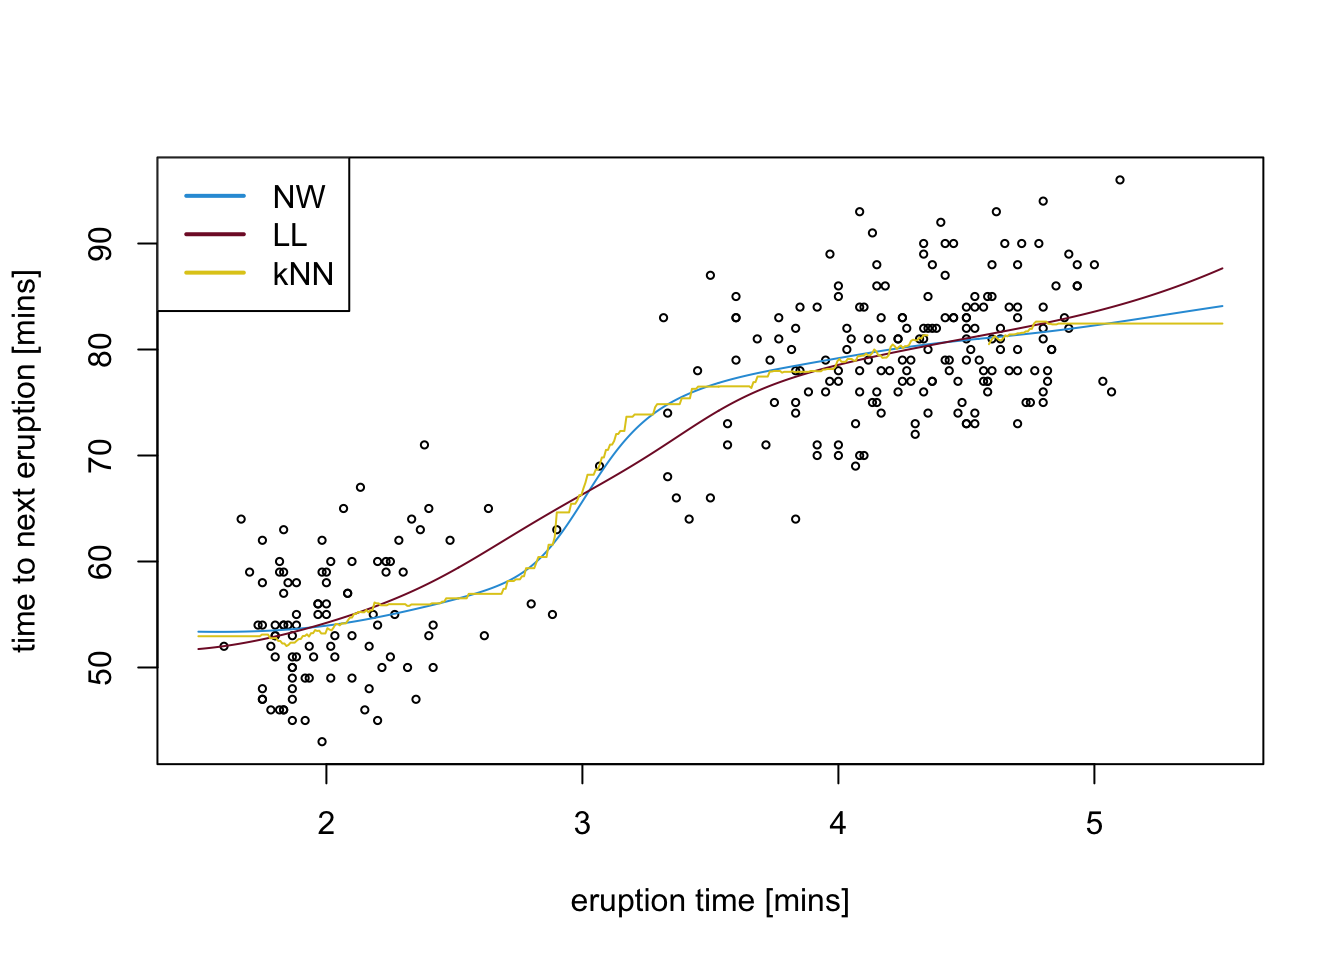
\includegraphics{MATH5714M_files/figure-latex/xv-summary-1.pdf}

\clearpage

\end{document}
